
\documentclass[11pt]{article}

% ----------------------------
% Packages
% ----------------------------
\usepackage[margin=1in]{geometry}
\usepackage{microtype}
\usepackage{mathtools, amssymb, amsthm, bm}
\usepackage{bbm}
\usepackage{graphicx}
\usepackage{booktabs}
\usepackage{multirow}
\usepackage{array}
\usepackage{enumitem}
\usepackage{hyperref}
\usepackage[nameinlink,noabbrev]{cleveref}
\usepackage{algorithm}
\usepackage{algpseudocode}
\usepackage{listings}
\usepackage{xcolor}
\usepackage{tikz}
\usetikzlibrary{arrows.meta, positioning, shapes.geometric, calc, fit}

% ----------------------------
% Basic formatting
% ----------------------------
\setlength{\parskip}{0.15em}
\setlength{\parindent}{0pt}
\linespread{1.0}

% ----------------------------
% Hyperref setup
% ----------------------------
\hypersetup{
  colorlinks=true,
  linkcolor=blue,
  citecolor=blue,
  urlcolor=blue
}

% ----------------------------
% Theorem environments
% ----------------------------
\theoremstyle{definition}
\newtheorem{definition}{Definition}[section]
\newtheorem{assumption}{Assumption}[section]
\newtheorem{example}{Example}[section]

\theoremstyle{plain}
\newtheorem{theorem}{Theorem}[section]
\newtheorem{proposition}{Proposition}[section]
\newtheorem{lemma}{Lemma}[section]
\newtheorem{corollary}{Corollary}[section]

\theoremstyle{remark}
\newtheorem{remark}{Remark}[section]

% ----------------------------
% Macros
% ----------------------------
\newcommand{\R}{\mathbb{R}}
\newcommand{\C}{\mathbb{C}}
\newcommand{\E}{\mathbb{E}}
\newcommand{\dd}{\,\mathrm{d}}
\newcommand{\ip}[2]{\left\langle #1, #2 \right\rangle}
\newcommand{\norm}[1]{\left\lVert #1 \right\rVert}
\newcommand{\opnorm}[1]{\left\lVert #1 \right\rVert_{\mathrm{op}}}
\newcommand{\Frob}[1]{\left\lVert #1 \right\rVert_{\mathrm{F}}}
\newcommand{\tr}{\operatorname{tr}}
\newcommand{\rank}{\operatorname{rank}}
\newcommand{\diag}{\operatorname{diag}}
\newcommand{\softmax}{\operatorname{softmax}}
\newcommand{\Lip}{\operatorname{Lip}}
\newcommand{\Id}{\mathbbm{1}}
\newcommand{\mc}[1]{\mathcal{#1}}
\newcommand{\bb}[1]{\mathbb{#1}}

% Typed spaces and graph notation
\newcommand{\Emb}{\mc{E}}
\newcommand{\Tok}{\mc{T}\mathrm{ok}}
\newcommand{\Nodes}{\mc{V}}
\newcommand{\Edges}{\mc{A}}
\newcommand{\src}{\operatorname{s}}
\newcommand{\tgt}{\operatorname{t}}
\newcommand{\Trop}{\mathbb{T}}
\newcommand{\Prob}{\mathbb{P}}
\newcommand{\Flow}{\mc{F}}
\newcommand{\Reward}{\mc{R}}

% ----------------------------
% Listings (code)
% ----------------------------
\lstdefinestyle{py}{
  language=Python,
  basicstyle=\ttfamily\footnotesize,
  keywordstyle=\bfseries,
  commentstyle=\itshape,
  stringstyle=\ttfamily,
  showstringspaces=false,
  breaklines=true,
  frame=single,
  columns=fullflexible,
  literate={≈}{{$\approx$}}1
}
\lstset{style=py}

% ----------------------------
% Title
% ----------------------------
\title{Composable Tropical Quivers for Learned Operators:\\
Transformer-General Architectures, Ergodic Embedding Flows, and Hybrid GFlowNet Search}


\author{Amelie Schreiber}

\date{\vspace{-1em}}

\begin{document}
\setcounter{tocdepth}{1}

\maketitle

\begin{abstract}
This paper develops a ground-up research program for \emph{composable learned operators} in which every internal module is viewed through a \emph{tropical lens} and every architecture is represented as a \emph{decorated quiver of embedding spaces}.
The organizing principle is boundary-aware:
discrete token spaces appear only at \emph{source encoder} vertices and \emph{sink decoder} vertices, while all intermediate computation lives in differentiable embedding spaces connected by general adapters, projections, cross-attention interfaces, residual merges, and neural-operator couplings.
This perspective is designed to cover standard transformers and their descendants---including ViT, DiT, SiT, multimodal fusion stacks, diffusion/flow transformers, state-space hybrids, and scientific foundation-model pipelines---while also extending to non-transformer modules.

The mathematical thesis is that modular deep systems should be studied as \emph{quivers of tropicalized operators}.
Piecewise-linear modules induce exact tropical rational maps and activation fans; transformer blocks become compositions of tropicalizable linear projections, piecewise-linear feed-forward layers, and tropical or locally tropicalized attention kernels; smooth modules admit local tropical charts on compact energy shells.
Composing such modules yields \emph{composed tropical spaces}: polyhedral atlases, tropical varieties, and scheme-like glued cell complexes attached to paths and cycles of the quiver.
This makes the geometry of composability explicit rather than hidden inside a global linear surrogate.

For cyclic quivers we develop a joint \emph{tropical-dynamical-ergodic} viewpoint.
Activation itineraries define symbolic dynamics on cell complexes; max-plus and subadditive cocycles quantify long-run growth; invariant measures describe occupancy of activation fans; and Navier--Stokes-inspired ``thought-fluid'' regularization constrains continuous Graph-of-Thought trajectories in embedding space.
The reward structure is integrated with \emph{hybrid continuous-discrete GFlowNets}: graph construction trajectories and continuous reasoning trajectories are both sampled with probability proportional to multiobjective rewards that favor high-quality solutions subject to explicit resource constraints.
We also show how recent activation-steering ideas, exemplified by the ``Assistant Axis,'' can be lifted to quiver-local tropical steering atlases that regulate both instantaneous embedding updates and long-run ergodic occupancy of activation regions.

The manuscript emphasizes formal definitions, rigorous propositions, implementation-oriented algorithms, and realistic examples.
These include continuous GoT reasoning GFlowNets, multimodal source/sink compositions linking NatureLM-style cross-domain sequence reasoning to MDGen-style SiT generative dynamics, and multi-model therapeutic design cycles that couple generators, evaluators, structure predictors, cell-state models, and phenotype or variant predictors through adapter-mediated embedding spaces.
The result is a tropical, quiver-theoretic, ergodic framework for architecture design and search that is intended to be both mathematically serious and practically actionable.
\end{abstract}

\tableofcontents
 

\section{Introduction}
\label{sec:intro}

Modern machine learning is no longer organized around a single network acting on a single modality.
Practical systems increasingly compose pretrained or jointly-trained modules:
transformers with patch, token, or latent inputs; diffusion/flow generators; cross-modal encoders; retrieval and memory controllers; neural operators; scientific oracles; and reward or ranking models.
The natural abstraction is not a layer stack but a \emph{typed graph of learned operators} whose edges carry adapters and whose strongly connected components implement iterative reasoning, generation, correction, or design.

This shift creates a mathematical gap.
We know how to optimize many modules individually, but we do not yet have a robust language for analyzing and searching over the \emph{compositions themselves}:
how embeddings are transported between modules, when cyclic executions remain stable, how architecture rewrites preserve useful structure, and how search over graphs should interact with continuous reasoning inside those graphs.
These questions become especially pressing when systems mix modalities and scales, as in scientific foundation models, multimodal diffusion stacks, or embedding-native Graph-of-Thought pipelines.

The central claim of this paper is that these systems should be modeled as \emph{decorated tropical quivers}.
Vertices represent learned operators acting on typed embedding spaces.
Arrows represent adapters or interface maps between those spaces.
Paths represent compositional programs.
Cycles represent dynamical systems.
Most importantly, each operator is studied through the polyhedral geometry induced by its activation structure, tropicalization, or local tropical chart.
This gives a representation that is exact for large classes of piecewise-linear components and still useful for smooth modules after local tropicalization.

We pursue four goals:
\begin{enumerate}[leftmargin=2em]
\item \textbf{Transformer generality.} The framework should cover self-attention, cross-attention, feed-forward, residual, routing, and latent-state updates in transformer families such as ViT, DiT, and SiT, while still extending to non-transformer operators.
\item \textbf{Boundary-aware composability.} Discrete token spaces should appear only at source encoders and sink decoders; everything in between should be treated as differentiable embedding-space computation linked by adapters.
\item \textbf{Tropical-dynamical rigor.} Cycles should be analyzed through tropical geometry, ergodic theory, and fluid-style regularization rather than through fragile global linear surrogates.
\item \textbf{Searchable architecture space.} The theory should support hybrid continuous-discrete GFlowNets whose rewards combine task quality with resource constraints and stability diagnostics.
\end{enumerate}

\subsection{Thesis and modeling choices}
\label{sec:thesis}

We adopt a deliberately \emph{implementation-first} abstraction.

\textbf{(i) Internal computation is embedding-native.}
Every non-boundary vertex $v$ acts on one or more typed embedding spaces:
\[
N_v : X_v \longrightarrow Y_v.
\]
The spaces $X_v,Y_v$ may be finite-dimensional token/tensor spaces, latent trajectory spaces, or discretized function spaces.
This includes transformer blocks, diffusion/flow blocks, MLPs, state-space modules, neural operators, and memory updates.

\textbf{(ii) Discrete tokenization appears only at the boundary.}
Source vertices encode environmental or symbolic inputs into embeddings,
\[
E_s:\Tok_s \to \Emb_{\alpha(s)},
\]
while sink vertices decode embeddings back into discrete outputs,
\[
D_t:\Emb_{\beta(t)} \to \Tok_t.
\]
Inside the quiver we treat all computation as differentiable transport and transformation in embedding space.
This cleanly separates differentiable composition from external symbolic interfaces.

\textbf{(iii) Edges are generalized adapters.}
Each arrow $e:u\to v$ carries a connector
\[
P_e:Y_u\to \pi_e(X_v),
\]
where $\pi_e(X_v)$ denotes the specific input port of $v$ addressed by $e$.
These connectors include dense and low-rank projections, cross-attention wiring, token reshaping, graph pooling, patchification/unpatchification, residual merges, and neural-operator restriction/prolongation maps.
The point is not to privilege a single adapter family, but to formalize \emph{any typical embedding-space linkage} used in practice.

\textbf{(iv) A modular architecture is a decorated quiver.}
The directed multigraph of boundary maps, internal operators, and connectors is the fundamental object.
Vertices carry nonlinear operator semantics; arrows carry linear, affine, or tropicalized transport semantics; and cycles carry dynamical semantics.
Quiver language is therefore not decorative:
it is the right level of abstraction for composability, mutation, diagnostics, and search.

\textbf{(v) Every learned operator is viewed through a tropical lens.}
For piecewise-linear modules we use exact tropical rational representations.
For tropical attention layers we use the tropical projective kernel and associated polyhedral decision structure.
For smooth modules we use local tropical charts on bounded energy sets.
This yields a common language in which composition becomes gluing of polyhedral pieces and recurrent execution becomes dynamics on a tropical cell complex.

\subsection{Transformer-general scope and boundary-aware modeling}
\label{sec:transformer-scope}

The theory is intended to subsume standard transformer variants rather than single out one architecture.
At a high level, a transformer block is a composition of:
\begin{enumerate}[leftmargin=2em]
\item typed linear projections,
\item a routing or attention mechanism,
\item piecewise-linear feed-forward subnetworks,
\item residual additions and layer-normalization-like coordinate changes, and
\item optional cross-attention or conditioning inputs.
\end{enumerate}
These pieces fit naturally into the quiver picture.
ViT uses image-patch source encoders and class-token sink decoders.
DiT and SiT use latent/image/noise embeddings together with conditioning edges and iterative denoising or flow cycles.
Multimodal transformers use multiple source encoders and one or more sink decoders connected through joint latent spaces.
The framework also allows hybrid stacks in which only some vertices are transformers and others are geometric, scientific, or retrieval-based modules.

\subsection{What this paper adds}
\label{sec:contribs}

The manuscript contributes a new theory, not just a new diagnostic.

\paragraph{A. Source/sink quiver semantics for embedding-native computation.}
We formalize architectures whose only discrete vertices are source encoders and sink decoders, while all intermediate vertices operate on continuous embeddings.
This makes it possible to reason formally about adapter-mediated compositions without collapsing internal dynamics back into token space.

\paragraph{B. A transformer-general tropicalization program.}
We show how transformer families fit the tropical-quiver viewpoint:
feed-forward blocks are cellwise affine, attention kernels may be tropical or locally tropicalized, and residual/cross-attention compositions glue these pieces into composed tropical spaces.
This covers ViT, DiT, SiT, multimodal transformers, and mixed systems that interleave transformer and non-transformer vertices.

\paragraph{C. Tropical dynamics and ergodic theory for cyclic quivers.}
We develop cyclic execution as dynamics on activation fans and composed tropical cell complexes.
Invariant measures, activation itineraries, max-plus cocycles, and subadditive growth rates replace global spectral heuristics.
We also strengthen the fluid viewpoint by treating Graph-of-Thought trajectories as continuous flows in embedding space, regularized by vorticity, divergence, and energy constraints inspired by fluid mechanics and Navier--Stokes analysis.

\paragraph{D. Hybrid continuous-discrete GFlowNet search.}
We formulate architecture search and internal reasoning search in a unified GFlowNet language.
Discrete actions add or mutate quiver structure; continuous actions propose connector parameters or reasoning displacements in embedding space.
Terminal probabilities are proportional to rewards that combine task quality, resource feasibility, and stability.

\paragraph{E. Realistic multimodal and scientific-design programs.}
We work through examples ranging from continuous GoT reasoning to multimodal scientific generation, including a NatureLM-to-MDGen composition and a richer therapeutic-design cycle linking generative, structural, cellular, and phenotypic models through shared embedding-space reasoning.

\paragraph{F. TokenGT-style graph universality and random-order decoding.}
We show how the sequence universality theorem for Transformers and the TokenGT graph-tokenization program combine to yield a graph-to-graph universality result for TokenGT-style transformers.
We also formalize a ProteinMPNN-style random-order autoregressive decoding scheme using graph tokens and explain why it is the right sink-decoding mechanism when outputs are graph-valued or structure-valued.

\paragraph{G. Ergodic tropical steering and stabilization.}
Motivated by recent assistant-axis activation steering, we show how one-dimensional residual-axis interventions lift to chartwise, quiver-local control rules.
The resulting formalism combines cellwise projection/capping, target corridors in learned steering coordinates, and invariant-measure objectives that tune long-run occupancy of activation regions rather than only one-step responses.

\subsection{Audit of the Koopman-centered draft}
\label{sec:audit}

An earlier version of the project already had several strong ingredients that remain central here:
\begin{itemize}[leftmargin=2em]
\item the \textbf{decorated-quiver formalism} for typed modular architectures,
\item the \textbf{connector/holonomy/Hodge} machinery for diagnosing interface mismatch on cycles,
\item the \textbf{ergodic} viewpoint that long-run execution statistics matter for cyclic graphs,
\item the \textbf{fluid and Navier--Stokes-inspired} regularization of continuous reasoning trajectories, and
\item the \textbf{continuous GFlowNet} approach to graph and connector search.
\end{itemize}
What changes in this manuscript is the organizing principle.
Koopman language is retained only as a foil that clarifies why a tropical-dynamical-ergodic program is better suited to heterogeneous modular systems.

\paragraph{Why the Koopman emphasis was too brittle.}
There are six structural issues.
\begin{enumerate}[leftmargin=2em]
\item \textbf{Observable dependence.} DMD/EDMD/deep-Koopman diagnostics depend strongly on the chosen feature map; poor features can create or erase apparent slow modes.
\item \textbf{Switching combinatorics are hidden.} The main source of nonlinearity in modular ReLU-style systems is activation switching across polyhedral regions. Koopman lifts obscure this combinatorics instead of organizing it.
\item \textbf{Nonstationarity is common.} During training, graph rewiring, connector updates, and controller changes continually alter the dynamics. Spectra estimated from short windows often reflect transient drift rather than persistent geometry.
\item \textbf{Localization is weak.} A problematic eigenvalue tells us something is wrong, but not \emph{which activation region, which connector, or which cell transition} causes the failure.
\item \textbf{Exactness is lost where it matters most.} For piecewise-linear modules there is already an exact algebraic description through tropical rational maps, activation fans, and tropical hypersurfaces; replacing this by an approximate global linear representation throws away usable structure.
\item \textbf{Composability is poorly encoded.} Koopman lifts linearize trajectories, but architecture design requires understanding how subgraphs glue, mutate, and share interfaces. Tropical quivers and their path algebras encode this directly.
\end{enumerate}

\paragraph{Design principles of the rewrite.}
The revised paper is organized around five principles:
\begin{enumerate}[leftmargin=2em]
\item \textbf{Exact when possible.} For piecewise-linear modules and connectors, use real tropical geometry exactly.
\item \textbf{Local when necessary.} For neural operators, fluid solvers, and smooth correctors, use local tropical charts on compact energy shells rather than a single global linearization.
\item \textbf{Ergodic rather than purely spectral.} Measure long-run behavior by invariant measures, activation itineraries, subadditive growth rates, and effective sample sizes.
\item \textbf{Boundary-aware and embedding-native.} Keep discrete tokenization at source/sink vertices and study internal computation in continuous embedding spaces.
\item \textbf{Composable by construction.} Treat graph rewrites, quiver mutation, adapter insertion, and connector fusion as first-class operations.
\item \textbf{Implementation first.} Every mathematical object should have a finite-dimensional estimator, a sparse linear-algebra representation, or a training-time penalty that can actually be used.
\end{enumerate}

\paragraph{The replacement in one sentence.}
We replace ``fit a global linear operator on observables'' by ``study the tropicalized quiver itself: its activation-cell atlas, path compositions, cyclic cocycles, invariant measures, and graph mutations''.

\subsection{Scope and non-goals}
We aim for a theory that can be implemented \emph{today}.
Accordingly, we avoid abstract machinery that does not translate into near-term algorithms.
We use only those algebraic, tropical, and ergodic tools that admit direct computation on graphs (cycle bases, holonomy/curvature surrogates, activation fans, tropical cycle means, Hodge spectra, Jacobian estimates) and directly inform training or debugging.

\subsection{Notation}
We denote by $\Emb_\alpha$ a typed embedding space (typically $\R^{d_\alpha}$ or a tensor space with explicit shape).
Vectors are column vectors.
For a linear map $A$, $\opnorm{A}$ is the operator norm induced by $\ell_2$ and $\Frob{A}$ is the Frobenius norm.
We write $\rho(A)$ for spectral radius and $\sigma_{\max}(A)$ for the largest singular value.
A directed multigraph (quiver) is $Q=(\Nodes,\Edges,\src,\tgt)$ with $\src(e),\tgt(e)\in\Nodes$.
The tropical semiring is $\Trop=(\R\cup\{-\infty\},\max,+)$ unless otherwise stated.
Discrete source or sink alphabets are denoted by $\Tok$ with task-specific subscripts.

\newpage

\section{Preliminaries and related work}
\label{sec:related}

This section provides only the prerequisites needed later and anchors them to practical ML design patterns.

\subsection{Modules, adapters, and interface learning}
Real modular systems typically compose components trained under different objectives, datasets, or modalities.
Interface learning therefore becomes central.
Common connectors include:
\begin{itemize}[leftmargin=2em]
\item \textbf{Linear probes and adapters:} learned linear heads or small bottleneck adapters that map one embedding space to another.
\item \textbf{Low-rank adaptations:} parameter-efficient updates such as LoRA-style low-rank decompositions of linear maps.
\item \textbf{Orthogonal/whitened alignments:} Procrustes maps and CCA-style projections used to align representations from different models.
\item \textbf{Cross-attention and token routing maps:} typed projections that send one embedding family into key/query/value or gating spaces of another module.
\item \textbf{Restriction, prolongation, and pooling operators:} maps that move between resolutions, modalities, or graph granularities.
\end{itemize}
These are implementable, differentiable, and amenable to algebraic diagnostics (norms, spectra, cycle consistency).

\subsection{Transformer blocks as learned operators}
\label{sec:prelim-transformers}

Transformer families differ in modality, conditioning, and time semantics, but they share a common operator skeleton.
At a coarse level, a block maps a typed token tensor $X\in\Emb_\alpha$ to another tensor in the same or a compatible type through
\[
X \mapsto X + \mc{A}(X;C) + \mc{F}(X;C),
\]
where $\mc{A}$ is self-attention, cross-attention, or routing-conditioned mixing, $\mc{F}$ is a feed-forward operator, and $C$ denotes optional conditioning signals.
ViT specializes this to image patches, DiT to latent denoising trajectories, and SiT/flow transformers to stochastic-interpolant or rectified-flow dynamics.
From the present viewpoint, each of these blocks is a vertex or a short path in the quiver.
The typed nature of the ports captures whether the block consumes patches, latent tokens, residue trajectories, or graph states.
The attached universality and TokenGT papers are especially relevant here:
Yun et al.\ prove sequence-to-sequence universality for Transformers \cite{YunBhojanapalliRawatKumarReddi2020}, while TokenGT shows that standard transformers acting on node and edge tokens already form a powerful graph-learning substrate \cite{KimNguyenMinChoLeeLeeHong2022}.

\subsection{Neural operators and infinite-dimensional views}
In scientific ML and operator learning, the primary object is a map between function spaces (e.g., PDE solution operators).
Architectures such as DeepONet and Fourier Neural Operators parameterize operators between Banach/Hilbert spaces.
Our framework treats both finite-dimensional networks and neural operators as instances of $N_v: X_v\to Y_v$; the only requirement is that $X_v,Y_v$ are normed spaces and that $N_v$ is differentiable almost everywhere for gradient-based training.

\subsection{Implicit layers and fixed-point models}
Cycles in computation graphs can be executed either by unrolling (explicit time steps) or by solving a fixed-point equation (implicit layers).
Deep equilibrium (DEQ) models and implicit neural layers provide a well-developed toolkit: contraction tests, Anderson/Broyden acceleration, and implicit differentiation.
We will reuse these tools, but in a \emph{graph} setting where multiple modules participate in a coupled fixed-point.

\subsection{Real tropical geometry, activation fans, and classification fans}
Two important tropical-geometry papers identify a strong exact structure for piecewise-linear networks:
feedforward ReLU systems represent \emph{tropical rational maps} \cite{ZhangNaitzatLim2018}, and the corresponding decision boundaries and parameter regions are organized by \emph{activation fans}, \emph{activation polytopes}, \emph{classification fans}, and real-tropical decision complexes \cite{BrandenburgLohoMontufar2024}.
For broader background on tropical hypersurfaces, polytopes, and fans, see \cite{MaclaganSturmfelsTropical}.
A new tropical-attention paper extends this picture directly into the transformer setting by replacing softmax attention with a tropical projective kernel and showing that multi-head tropical attention inherits sharp polyhedral decision structure together with strong algorithmic expressivity \cite{HashemiPasqueTeskaYoshida2025}.
These objects are better suited than global spectral surrogates when the dominant difficulty is activation switching, routing, and polyhedral composition.
We will adapt them from standard feedforward classification to \emph{cyclic quivers}: cell decompositions become dynamical state spaces, activation itineraries become symbolic dynamics, and tropical hypersurfaces become concrete instability boundaries for connectors, recurrent message passing, and graph rewrites. 

\subsection{Cluster-algebra and mutation viewpoints on quivers}
\label{sec:cluster}

Cluster-algebra language is not used here as a full formal substrate for neural architectures, but it provides a valuable design analogy.
Quiver mutation, seed mutation, and coordinate changes organize how one representation of a combinatorial object is transformed into another while preserving structured algebraic relations.
In the spirit of the cluster-algebra literature and Schiffler's expository work on quivers, mutations, and cluster categories, we interpret architecture rewrites---inserting adapters, replacing a subpath by an equivalent block, or changing a routing factorization---as \emph{neural quiver mutations} that should preserve selected invariants or improve rewards while maintaining typed compatibility \cite{FominWilliamsZelevinsky2016,SchifflerClusterNotes,SchifflerQuiverReps}.
This perspective is especially useful when later discussing graph rewrites, connector fusion, and architecture search, but there is an important distinction to be made here: our version is \emph{learned}, whereas the standard mutations discussed in the cluster algebra literature is \emph{not}. 

\subsection{GFlowNets and architecture search over graphs}
GFlowNets are generative models trained to sample objects with probability proportional to a reward.
They have been used for combinatorial generation (molecules, sequences) and can be adapted to graph spaces (architectures).
We focus on \emph{continuous/hybrid} GFlowNets that support both discrete structure (graph edges) and continuous parameters (connector matrices).
Compared with standard neural architecture search, the GFlowNet view emphasizes \emph{diverse} high-reward samples and supports explicit multiobjective trade-offs.
In this paper we also use the same formalism \emph{inside} a fixed quiver:
continuous Graph-of-Thought trajectories are treated as flow objects in embedding space, with terminal trajectory density proportional to a reward that depends jointly on task quality and resource feasibility.

\subsection{Positioning}
The present work sits at the intersection of:
\begin{itemize}[leftmargin=2em]
\item \textbf{Systems-oriented modular deep learning} (adapters, tool graphs, multi-model stacks),
\item \textbf{Operator learning and tropical/ergodic analysis} for cyclic modular systems,
\item \textbf{Graph-based architecture search} (GFlowNets with continuous actions),
\item \textbf{Algebraic structure of composition} (quivers/path algebras) used as a design calculus rather than an abstract end in itself.
\end{itemize}
Recent activation-steering work is also directly relevant:
the Assistant Axis of \cite{AnthropicAssistantAxis2026,LuGallagherMichalaFishLindsey2026} gives a concrete example of low-dimensional embedding-space control, which we later generalize from a single-axis language-model intervention to chartwise steering on cyclic tropical quivers.

\newpage

\section{Decorated quivers for modular deep systems}
\label{sec:quiver}

We now define the core object: a computation graph where vertices are nonlinear modules and edges are learnable connectors.

\subsection{Typed embedding spaces and ports}
\label{sec:typed}

Let $\mc{T}$ be a set of \emph{types}.
A type $\alpha\in\mc{T}$ corresponds to a concrete tensor space $\Emb_\alpha$, including shape/layout conventions.
Typical examples:
\begin{itemize}[leftmargin=2em]
\item $\Emb_{\text{text}}=\R^{L\times d_\text{text}}$ for token embeddings,
\item $\Emb_{\text{image}}=\R^{H\times W\times d_\text{img}}$ for image features,
\item $\Emb_{\text{state}}=\R^{d}$ for a world-model latent state,
\item $\Emb_{\text{field}}=L^2(\Omega;\R^{c})$ for a PDE field (discretized in practice).
\end{itemize}

\subsubsection{Smooth modality changes and joint embedding spaces}
\label{sec:modal-smooth}

Typed ports make heterogeneous modalities explicit, but \emph{do not} require matched dimensions or shared bases.
A connector $P_e$ is precisely the place where we learn a \emph{differentiable} change-of-representation between modalities while staying in continuous spaces.
Two implementable wiring patterns recur:

\begin{enumerate}[leftmargin=2em]
\item \textbf{Lift--fuse--project via a joint space.}
Introduce a joint type $\text{joint}$ with embedding space $\Emb_{\text{joint}}$.
Use linear projections $L_{u\to \text{joint}}$ and $R_{\text{joint}\to v,i}$ so that the effective connector factors as
\[
P_{u\to v} \;=\; R_{\text{joint}\to v,i}\circ F_{\text{joint}}\circ L_{u\to \text{joint}},
\]
where $F_{\text{joint}}$ is a small \emph{vertex} (e.g., cross-attention, pooling, message passing) that performs fusion in the joint space.
Keeping $F_{\text{joint}}$ as a vertex avoids hiding expressive nonlinearities inside edges while remaining fully differentiable.

\item \textbf{Product-state trajectories across modalities.}
Maintain a state $z=(z^{(\text{text})},z^{(\text{vision})},z^{(\text{control})},\ldots)\in \prod_{\alpha}\Emb_{\alpha}$ and use block-sparse connectors that only touch the relevant factors.
This makes ``reasoning trajectories'' well-defined in the \emph{product} embedding space and enables smooth, modality-switching computation: arrows simply project/lift between factors or into a joint space.
\end{enumerate}

When we analyze cyclic behavior we linearize \emph{at vertices}: each nonlinear module contributes a Jacobian $J_v$ (obtained by autodiff), while connectors are already linear.
Thus modality changes remain smooth in the sense that they have well-defined Jacobians everywhere in the interior of the quiver; discontinuities are confined to designated boundary vertices (encoders/decoders).

A module has \emph{ports} (inputs/outputs) labeled by types.

\begin{definition}[Module vertex]
A \emph{module} is a differentiable map
\[
N_v:\; X_v \to Y_v,
\qquad
X_v = \bigoplus_{i=1}^{m_v}\Emb_{\alpha_i(v)},
\qquad
Y_v = \Emb_{\beta(v)} ,
\]
where $\alpha_i(v),\beta(v)\in\mc{T}$.
We treat $\oplus$ as a structured concatenation/direct sum (in code: concatenation along feature axis, packing into a tuple, or a named dict).
\end{definition}

\begin{definition}[Connector edge]
Given modules $u,v$, a directed edge $e:u\to v$ selects an input port index $i(e)\in\{1,\dots,m_v\}$ and carries a learnable connector operator
\[
P_e:\; Y_u \to \Emb_{\alpha_{i(e)}(v)}.
\]
Unless otherwise stated, we assume $P_e$ is linear or affine:
$P_e(z)=A_e z + b_e$ with a matrix/tensor $A_e$ (possibly structured) and bias $b_e$.
\end{definition}

\paragraph{Why emphasize (affine) linear connectors?}
They are ubiquitous (probes, adapters, LoRA, $1\times 1$ conv projections), cheap relative to nonlinear modules, and they admit strong diagnostics:
operator norms, conditioning, cycle consistency, and spectral constraints.
When a richer interface is needed, the recommended pattern is to \emph{promote} it to a module vertex (e.g., cross-attention as a vertex) rather than overloading the edge semantics.

\subsection{Decorated quiver definition}
\label{sec:decorated-quiver}

A quiver is a directed multigraph.

\begin{definition}[Decorated quiver]
A \emph{decorated quiver} is a tuple
\[
\mc{Q}=(Q,\{N_v\}_{v\in\Nodes},\{P_e\}_{e\in\Edges}),
\qquad Q=(\Nodes,\Edges,\src,\tgt),
\]
where each vertex $v\in\Nodes$ carries a module $N_v$ and each edge $e\in\Edges$ carries a connector $P_e$ landing in a specific port of $\tgt(e)$.
\end{definition}

In practice, a decorated quiver is a typed directed graph plus a parameter store for modules and connectors.


\subsection{Boundary vertices and embedding-native interiors}
\label{sec:boundary}

Many practical systems interface with \emph{non-embedding} artifacts: discrete text tokens, symbolic API calls, simulator states, or measurements returned by external tools.
These interfaces are useful, but they introduce discontinuities (e.g., sampling tokens, executing a program) that are not compatible with end-to-end backpropagation.

Our modeling convention is therefore:

\begin{quote}
\emph{All interior vertices and edges of the decorated quiver operate on continuous embedding spaces and are differentiable.
Any conversion to/from discrete artifacts occurs only at designated \textbf{boundary} vertices, which are treated as roots (inputs) or sinks (outputs).}
\end{quote}

\paragraph{Text as a boundary interface.}
Let $\mathrm{ENC}$ map an external token sequence into an embedding sequence (a linear embedding lookup followed by an encoder).
This is a root boundary: gradients are taken with respect to encoder parameters, not with respect to the discrete token indices.
Similarly, let $\mathrm{DEC}$ map an embedding to logits over a vocabulary.
Training can remain fully differentiable by placing losses on logits (cross-entropy, KL to a teacher distribution); the discontinuous step (argmax/sampling) is deferred to the sink boundary at inference time.

\paragraph{Tools and simulators.}
A tool call is naturally a sink boundary (an action emitted to the environment), and the tool's return value is a root boundary (an external observation re-embedded into the graph).
The quiver formalism still applies on either side of the boundary, but gradients do not flow through the environment; use distillation, surrogate models, or policy-gradient estimators if learning depends on these calls.

This boundary discipline is particularly important for reasoning-and-memory loops: decoding intermediate ``thoughts'' into discrete text and re-encoding them inserts avoidable discontinuities.
The GoT memory construction in \cref{sec:case-studies} keeps the entire internal loop in embedding space, and uses boundary vertices only for initial encoding and final decoding.


\begin{figure}[t]
\centering
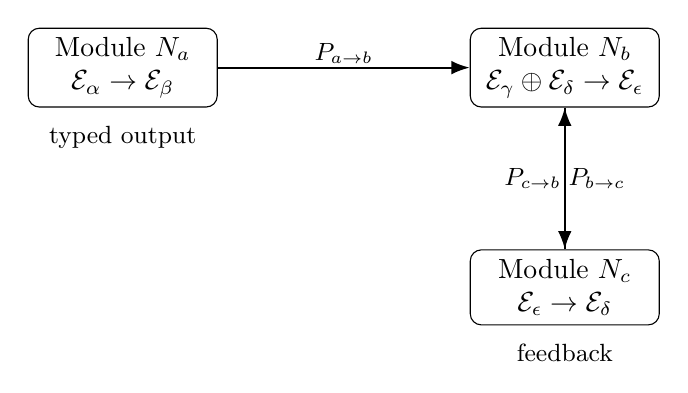
\begin{tikzpicture}[
  node/.style={draw, rounded corners, minimum width=2.4cm, minimum height=0.9cm, align=center},
  edge/.style={-Latex, thick},
  lab/.style={font=\small, inner sep=1pt}
]
\node[node] (A) {Module $N_a$\\$\Emb_{\alpha}\to\Emb_{\beta}$};
\node[node, right=3.2cm of A] (B) {Module $N_b$\\$\Emb_{\gamma}\oplus \Emb_{\delta}\to\Emb_{\epsilon}$};
\node[node, below=1.8cm of B] (C) {Module $N_c$\\$\Emb_{\epsilon}\to\Emb_{\delta}$};

\draw[edge] (A) -- node[lab, above] {$P_{a\to b}$} (B);
\draw[edge] (B) -- node[lab, right] {$P_{b\to c}$} (C);
\draw[edge] (C) -- node[lab, left] {$P_{c\to b}$} (B);

\node[lab, below=0.2cm of A] {typed output};
\node[lab, below=0.2cm of C] {feedback};
\end{tikzpicture}
\caption{A decorated quiver: vertices are nonlinear modules; edges are learnable connectors.
The $b\leftrightarrow c$ cycle can be executed by unrolling or as a fixed point.}
\label{fig:quiver}
\end{figure}

\subsection{Execution semantics: acyclic graphs}
\label{sec:acyclic}

If $Q$ is acyclic (a DAG), execution is standard.
Each vertex aggregates its incoming messages by port; missing ports are filled by external inputs or a default value.

Let $\mathrm{In}(v)=\{e\in\Edges:\tgt(e)=v\}$ denote incoming edges and let $\mc{E}_v=(\Emb_{\alpha_1(v)},\dots,\Emb_{\alpha_{m_v}(v)})$ be the input port spaces.
Execution computes, for each $v$,
\[
x_v^{(i)} = \sum_{e\in\mathrm{In}(v):\, i(e)=i} P_e(y_{\src(e)}) \;+\; x_{v,\mathrm{ext}}^{(i)},
\qquad
y_v = N_v(x_v^{(1)},\dots,x_v^{(m_v)}).
\]
Summation above is one choice; alternatives include concatenation, attention-based pooling, or learned gating.
When the aggregator is nonlinear, we treat it as part of $N_v$.

\begin{algorithm}[t]
\caption{Evaluate a decorated quiver (DAG case)}
\label{alg:eval-dag}
\begin{algorithmic}[1]
\Require DAG $Q=(\Nodes,\Edges)$ with modules $N_v$, connectors $P_e$, external inputs $x_{v,\mathrm{ext}}$
\Ensure Outputs $\{y_v\}_{v\in\Nodes}$
\State topological order $\pi \gets \mathrm{TopoSort}(Q)$
\For{$v$ in $\pi$}
  \For{$i=1$ to $m_v$}
    \State $x_v^{(i)} \gets x_{v,\mathrm{ext}}^{(i)}$
  \EndFor
  \For{edge $e$ with $\tgt(e)=v$}
    \State $u \gets \src(e)$; $i\gets i(e)$
    \State $x_v^{(i)} \gets x_v^{(i)} + P_e(y_u)$
  \EndFor
  \State $y_v \gets N_v(x_v^{(1)},\dots,x_v^{(m_v)})$
\EndFor
\end{algorithmic}
\end{algorithm}

\subsection{Execution semantics: cyclic graphs}
\label{sec:cycles}

Cycles represent feedback (planning loops), iterative refinement, or sampling (diffusion steps).
We support two execution models.

\paragraph{Unrolled semantics.}
Choose a horizon $T$ and unroll each cycle into $T$ iterations, producing a DAG.
This is appropriate when the algorithmic semantics of the system is explicitly iterative (e.g., $T$ diffusion steps, $T$ policy improvement steps).

\paragraph{Fixed-point semantics.}
Treat cyclic subgraphs as an implicit system and solve for a fixed point.
This captures equilibria, recurrent steady-state inference, and implicit layers.

We formalize fixed points because they yield useful \emph{stability criteria} and \emph{implicit differentiation}.

Let $\Nodes_\mathrm{state}\subseteq\Nodes$ denote vertices whose outputs are part of the recurrent state.
Define the product state space
\[
Z := \prod_{v\in \Nodes_\mathrm{state}} Y_v.
\]
Given external inputs and current state $z\in Z$, one full ``graph update'' defines a map
\[
\Phi_{\theta,P}: Z \to Z,
\]
where $\theta$ collects all module parameters and $P$ all connector parameters.
A fixed point is $z^\star$ such that $z^\star=\Phi_{\theta,P}(z^\star)$.

\begin{assumption}[Regularity]
For fixed external inputs, $\Phi_{\theta,P}$ is continuous and (locally) Lipschitz on $Z$.
This holds when modules are Lipschitz and connectors are bounded linear/affine maps.
\end{assumption}

\begin{theorem}[Convergence under contraction]
\label{thm:contraction}
Let $(Z,\norm{\cdot})$ be complete.
If $\Phi_{\theta,P}$ is a contraction, i.e.,
there exists $0\le L<1$ such that
\[
\norm{\Phi(z)-\Phi(z')} \le L\norm{z-z'}\qquad \forall z,z'\in Z,
\]
then a unique fixed point $z^\star$ exists and Picard iteration $z_{t+1}=\Phi(z_t)$ converges linearly to $z^\star$ for any initialization.
\end{theorem}

\paragraph{Graph-level Lipschitz bound.}
A sufficient (conservative) condition for contraction can be obtained from local Lipschitz constants.
Suppose each module $N_v$ is $L_v$-Lipschitz and each connector $P_e$ has operator norm $\opnorm{P_e}$.
For a given choice of aggregation rule, one can bound the Jacobian of $\Phi$ in terms of products of $\opnorm{P_e}$ and $L_v$ along paths within the recurrent subgraph.
\Cref{sec:stability} and \cref{app:fixed-point} provide computable bounds and practical tests.

\paragraph{Implicit differentiation.}
When training uses the fixed point $z^\star(\theta,P)$, gradients can be computed without backpropagating through all unrolled iterations by using the implicit function theorem.
This yields memory savings and supports long-horizon cycles when contraction holds (\cref{app:fixed-point}).

\newpage

\section{Transformer blocks, adapters, and composed tropical spaces}
\label{sec:transformer-tropical}

This section makes explicit what has so far been implicit:
the tropical-quiver formalism is intended to cover transformer families directly, not merely as motivating examples.
We therefore describe a generic transformer block as a decorated-quiver gadget, explain how tropical attention fits inside it, and formalize the composed tropical spaces created when multiple blocks and adapters are glued together.

\subsection{A generic transformer vertex}
\label{sec:generic-transformer}

Let $\Emb_\alpha=\R^{L\times d}$ be a typed token space, where the semantic meaning of the $L$ slots depends on the application:
patches for ViT, latent/image tokens for DiT, residue-time tokens for SiT-based molecular trajectory models, or multimodal scientific sequences in a model such as NatureLM.
A \emph{generic transformer vertex} is a quiver vertex whose internal map factors as
\[
N_v
=
R_v \circ \Bigl(\Id + \mc{F}_v \Bigr)\circ \Bigl(\Id + \mc{A}_v\Bigr)\circ L_v,
\]
where:
\begin{itemize}[leftmargin=2em]
\item $L_v$ and $R_v$ are typed linear or affine port maps,
\item $\mc{A}_v$ is self-attention, cross-attention, or a routing/mixing block,
\item $\mc{F}_v$ is a feed-forward or MLP block, typically piecewise affine,
\item residual additions are represented explicitly by the two identity summands.
\end{itemize}
This factorization is not meant to mirror every implementation detail;
it isolates the pieces that matter mathematically for tropicalization and composability.

\begin{definition}[Transformer-compatible decorated quiver]
A decorated quiver is \emph{transformer-compatible} if every internal vertex admits a factorization into typed linear lifts, a routing/attention core, a piecewise-linear or locally tropicalizable nonlinear block, and a residual merge.
\end{definition}

The definition is intentionally broad.
It includes standard encoders/decoders, diffusion transformers, flow transformers, multimodal co-attention blocks, mixture-of-experts routers, and memory-attention hybrids.

\subsection{Tropical attention as a first-class quiver primitive}
\label{sec:tropical-attention}

The tropical-attention paper that helped inspire part of this project provides an important bridge:
attention itself can be defined in tropical projective space, yielding a polyhedral, non-expansive, sharp alternative to softmax attention \cite{HashemiPasqueTeskaYoshida2025}.
For our purposes, there are three consequences.

\paragraph{(1) Tropical attention is already quiver-native.}
Queries, keys, and values are produced by typed projections, so a self-attention head naturally decomposes into arrows
\[
X \xrightarrow{W_Q} Q,\qquad
X \xrightarrow{W_K} K,\qquad
X \xrightarrow{W_V} V,
\]
followed by a fusion vertex computing the attention update.
Cross-attention is identical except that source and target token spaces differ.

\paragraph{(2) The induced geometry is polyhedral.}
Because the tropical projective kernel is piecewise-linear and respects the polyhedral decision structure of the inputs, it harmonizes with the activation-fan viewpoint used throughout this manuscript.
In particular, when attention is tropical, the entire transformer block becomes a composition of tropical or cellwise-affine maps except for smooth normalization or gating operations, which can be locally tropicalized.

\paragraph{(3) Expressivity scales compositionally.}
The universal-approximation and transitive-closure perspective in \cite{HashemiPasqueTeskaYoshida2025} supports the use of tropical attention not only in algorithmic reasoning, but also as a compositional kernel for architecture search.
From the quiver viewpoint this means that high-level graph search can be phrased in terms of how many tropical-routing primitives, adapter insertions, and residual paths are needed for a task.

\begin{proposition}[Transformer blocks are tropical rational after tropical attention and piecewise-linear feed-forwards]
\label{prop:transformer-tropical}
Assume that:
\begin{enumerate}[leftmargin=2em]
\item all query, key, value, output, and adapter maps are affine,
\item the attention core is tropical attention,
\item feed-forward subblocks are piecewise affine with finitely many regions, and
\item normalization/gating maps are either affine or replaced by local affine charts on a compact set.
\end{enumerate}
Then the resulting block map is coordinatewise tropical rational on each chart and therefore defines a finite activation fan on that chart.
\end{proposition}

\begin{proof}[Proof sketch]
Affine maps are tropical rational.
Tropical attention is piecewise-linear in tropical projective coordinates by construction.
Piecewise-affine feed-forward subnetworks are tropical rational by the ReLU/tropical correspondence.
Composition preserves piecewise-affine structure after common refinement of the underlying fans.
\end{proof}

\subsection{Standard softmax attention as a locally tropicalizable operator}
\label{sec:softmax-local-tropical}

Not every deployed model uses tropical attention.
The framework therefore also needs a way to analyze standard softmax transformers without pretending they are already tropical in an exact sense.
Our stance is pragmatic:
softmax attention is treated as a \emph{locally tropicalizable} operator.
On bounded subsets of logit space, one may:
\begin{enumerate}[leftmargin=2em]
\item approximate the softmax map by a cellwise-affine surrogate,
\item isolate dominant heads or dominant token cones to obtain a local tropical chart, or
\item analyze the pre-attention and post-attention maps tropically while treating the softmax core as a smooth change of coordinates.
\end{enumerate}
This is weaker than exact tropicality, but still preserves the quiver-level compositional analysis.
The manuscript therefore applies to contemporary transformers regardless of whether they use softmax attention, tropical attention, linear attention, or routing-based kernels.

\subsection{Composed tropical spaces from adapters and residual paths}
\label{sec:composed-tropical-spaces}

When several module vertices are linked by adapters, the resulting geometry is not simply ``the tropicalization of one layer''.
Instead, each path through the quiver induces its own tropical chart, and joint execution glues these charts together.
This motivates the following language.

\begin{definition}[Composed tropical space of a quiver]
Let $\mc{Q}$ be a decorated quiver with internal vertices that are tropical or locally tropicalized on a family of charts.
The \emph{composed tropical space} $\mc{X}_{\mathrm{trop}}(\mc{Q})$ is the polyhedral atlas obtained by gluing the cell complexes of all admissible path compositions along the adapter maps and shared residual coordinates.
\end{definition}

This object is intentionally scheme-like rather than purely fan-like:
different regions of the quiver may admit different local charts, and adapter-mediated gluing may identify subcomplexes only after a change of coordinates.
For implementation, however, the important point is simple:
the composed tropical space is a finite combinatorial object after restricting to an empirical support of visited cells.

\paragraph{Why this matters.}
The composed tropical space captures:
\begin{itemize}[leftmargin=2em]
\item where representation mismatch occurs between modules,
\item where routing or attention decisions change sharply,
\item how residual shortcuts alter the effective geometry of a block stack, and
\item which subgraphs should be mutated, fused, or pruned during architecture search.
\end{itemize}

\subsection{TokenGT-style tokenization of graph states}
\label{sec:tokengt-setup}

The preceding discussion treated transformer inputs abstractly as typed token spaces.
For graph-valued states and graph-valued outputs, a particularly relevant concrete instantiation is the Tokenized Graph Transformer (TokenGT) view \cite{KimNguyenMinChoLeeLeeHong2022}.
Given a graph, one treats all nodes and edges as tokens, augments them with type identifiers and node identifiers, and then applies a standard Transformer encoder.
The TokenGT paper proves that this seemingly simple representation is already highly expressive:
with suitable identifiers, self-attention over node and edge tokens can approximate the equivariant linear primitives underlying higher-order invariant graph networks.

For the purposes of this manuscript, TokenGT is important in two ways.
First, it shows that graph-structured latent states fit naturally into the same boundary-aware transformer formalism as text, image patches, or trajectory tokens.
Second, it suggests that the internal quiver state of a modular system may itself be graph-valued without leaving the tropical-transformer framework:
a graph-of-thought memory, a molecular interaction graph, or a multi-agent planning graph can be handled by node/edge tokenization rather than by ad hoc message passing.

This observation will let us upgrade the universality discussion from sequence-to-sequence maps to graph-to-graph maps in the next section.
It also motivates an order-agnostic autoregressive decoding scheme for graph outputs, where the model predicts node or edge labels in a random order instead of committing to a brittle left-to-right serialization.

\subsection{Examples: ViT, DiT, and SiT in quiver form}
\label{sec:vit-dit-sit}

\paragraph{ViT.}
A ViT pipeline is a quiver with an image-patch source encoder, a sequence of transformer vertices on patch embeddings, and one or more sink decoders for labels or dense outputs.
Patch embedding is a source map into $\Emb_{\text{patch}}$.
The class token, if present, is simply a distinguished coordinate in the embedding space.
All internal operations are embedding-native.

\paragraph{DiT.}
A DiT-style latent diffusion model forms a cyclic quiver:
noise or latent tokens enter through a source encoder, time and conditioning edges feed a stack of transformer vertices, and the denoising update returns to the latent state.
The iterative denoising loop is therefore a cyclic decorated quiver analyzed by the tropical-dynamical machinery of \cref{sec:tropical-cycle-dynamics}.

\paragraph{SiT and flow-transformer models.}
SiT-style stochastic-interpolant or flow models differ from DiT mainly in the semantics of time and velocity prediction.
From the quiver viewpoint this changes the vector field attached to the cycle, but not the source/sink boundary discipline or the adapter semantics.
This is especially important for models such as MDGen, where residue-time tokens and conditioning embeddings coexist in a structured trajectory space.

\begin{figure}[t]
\centering
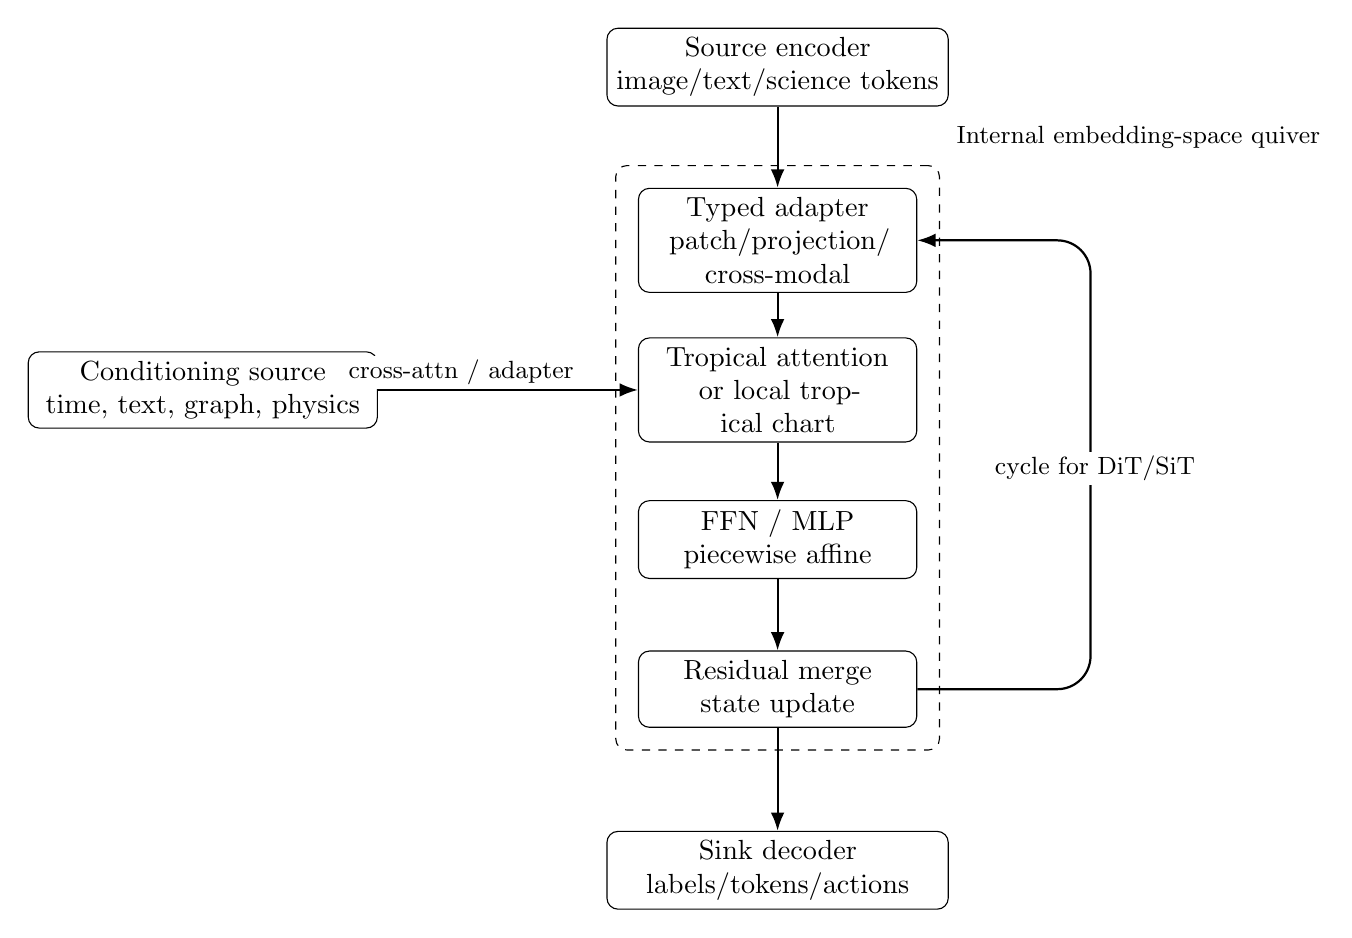
\begin{tikzpicture}[
  inode/.style={draw, rounded corners, minimum height=0.95cm, text width=3.3cm, align=center},
  bnode/.style={draw, rounded corners, minimum height=0.95cm, text width=4.1cm, align=center},
  cnode/.style={draw, rounded corners, minimum height=0.95cm, text width=4.2cm, align=center},
  edge/.style={-Latex, thick},
  box/.style={draw, dashed, rounded corners, inner sep=8pt},
  lab/.style={font=\small, fill=white, inner sep=1.5pt}
]
\node[bnode] (src1) at (0,5.4) {Source encoder\\image/text/science tokens};
\node[inode] (proj) at (0,3.2) {Typed adapter\\patch/projection/\\cross-modal};
\node[inode] (attn) at (0,1.3) {Tropical attention\\or local tropical chart};
\node[inode] (ffn) at (0,-0.6) {FFN / MLP\\piecewise affine};
\node[inode] (res) at (0,-2.5) {Residual merge\\state update};
\node[bnode] (sink) at (0,-4.8) {Sink decoder\\labels/tokens/actions};
\node[cnode] (cond) at (-7.3,1.3) {Conditioning source\\time, text, graph, physics};

\draw[edge] (src1) -- (proj);
\draw[edge] (proj) -- (attn);
\draw[edge] (attn) -- (ffn);
\draw[edge] (ffn) -- (res);
\draw[edge] (res) -- (sink);
\draw[edge] (cond.east) -- node[lab, above, pos=0.32] {cross-attn / adapter} (attn.west);
\draw[edge, rounded corners=12pt] (res.east) -- ++(2.2,0) |- (proj.east);
\node[lab, anchor=west] at (2.7,0.3) {cycle for DiT/SiT};

\node[box, fit=(proj)(attn)(ffn)(res)] (embedbox) {};
\node[lab, anchor=west] at ($(embedbox.north east)+(0.15,0.35)$) {Internal embedding-space quiver};
\end{tikzpicture}
\caption{Transformer-general view of a learned operator quiver.
Discrete objects appear only at source/sink boundaries; all internal computation is an adapter-linked embedding-space quiver.
ViT corresponds to a mostly acyclic version, while DiT and SiT add explicit cycles through the latent state.}
\label{fig:transformer-quiver}
\end{figure}

\subsection{Adapters as tropical gluing morphisms}
\label{sec:adapter-gluing}

Adapters are often treated as a minor engineering detail.
In this manuscript they play a more structural role:
they are the \emph{gluing morphisms} that turn a collection of local tropical spaces into a composed tropical quiver.
This is true whether the adapter is a dense projection, LoRA-like low-rank map, cross-attention bridge, or graph pooling layer.

\begin{definition}[Adapter admissibility]
An adapter $P_e:Y_u\to X_v$ is \emph{admissible} for tropical composition if it satisfies:
\begin{enumerate}[leftmargin=2em]
\item typed compatibility,
\item bounded operator norm on the occupied region,
\item finite-rank or finite-chart description on the occupied region, and
\item differentiability almost everywhere.
\end{enumerate}
\end{definition}

These conditions are mild enough to cover the adapters used in modern practice and strong enough to support the diagnostics developed later.

\subsection{Mutation and rewrite moves for transformer quivers}
\label{sec:transformer-mutations}

The cluster-algebra analogy from \cref{sec:cluster} becomes concrete once we decide what counts as a legitimate architecture mutation.
Examples include:
\begin{itemize}[leftmargin=2em]
\item inserting an adapter to mediate a difficult interface,
\item replacing a long path by a fused block with the same typed signature,
\item splitting one attention vertex into multiple heads or branches,
\item lifting a hidden nonlinear edge transform into an explicit vertex,
\item replacing softmax attention by tropical attention or by a local tropical surrogate for diagnostic purposes.
\end{itemize}
Each move changes the quiver, and typically also its composed tropical space.
The search problem in later sections can therefore be interpreted as a stochastic exploration of mutation sequences guided by reward.

\newpage

\section{TokenGT universality and random-order graph decoding}
\label{sec:tokengt-universality}

The previous section argued that transformer blocks fit naturally into the tropical-quiver viewpoint.
We now add a sharper theorem-level statement motivated by the following two papers:
\begin{enumerate}[leftmargin=2em]
\item the sequence universality theorem of Yun et al.\ \cite{YunBhojanapalliRawatKumarReddi2020}, and
\item the graph-tokenization and graph-expressivity result of TokenGT \cite{KimNguyenMinChoLeeLeeHong2022}.
\end{enumerate}
Together they imply that TokenGT-style transformers are not merely graph classifiers or graph encoders.
Under the same compactness and continuity assumptions used in the sequence literature, they are also universal \emph{graph-to-graph} function approximators, rather than only being universal sequence-to-sequence function approximators. This matters directly for the present manuscript because many source/sink interfaces and many internal thought states are graph-valued. 

\subsection{Graph tokenization as a boundary map}
\label{sec:graph-tokenization}

Fix integers $n_{\max},m_{\max}\ge 1$ and let $\mc{G}_{n_{\max},m_{\max}}^{\mathrm{in}}$ denote a compact family of attributed input graphs with at most $n_{\max}$ nodes and $m_{\max}$ edges, represented with padded continuous node and edge features.
Likewise let $\mc{G}_{\bar n,\bar m}^{\mathrm{out}}$ be a compact family of output graphs.
We write $\mathrm{Tok}_{\mathrm{in}}$ and $\mathrm{Tok}_{\mathrm{out}}$ for TokenGT-style tokenization maps:
each graph is sent to a padded sequence of node and edge tokens augmented by node identifiers and type identifiers.
The image spaces are compact subsets
\[
K_{\mathrm{in}} \subset \R^{d_{\mathrm{in}}\times L_{\mathrm{in}}},
\qquad
K_{\mathrm{out}} \subset \R^{d_{\mathrm{out}}\times L_{\mathrm{out}}},
\]
where $L_{\mathrm{in}}=n_{\max}+m_{\max}$ and $L_{\mathrm{out}}=\bar n+\bar m$ after padding.

\begin{definition}[Graph-token equivariance]
Let $F:\mc{G}_{n_{\max},m_{\max}}^{\mathrm{in}}\to \mc{G}_{\bar n,\bar m}^{\mathrm{out}}$.
We say that $F$ is \emph{graph-equivariant} if relabeling the nodes and edges of the input relabels the nodes and edges of the output in the corresponding way.
The induced token map is
\[
\widetilde F
:=
\mathrm{Tok}_{\mathrm{out}}\circ F\circ \mathrm{Tok}_{\mathrm{in}}^{-1}
:
K_{\mathrm{in}}\to K_{\mathrm{out}}.
\]
\end{definition}

The role of TokenGT identifiers is crucial here:
they keep the token representation faithful to graph incidence data even though the Transformer only sees a sequence of tokens.
As emphasized in \cite{KimNguyenMinChoLeeLeeHong2022}, the node and type identifiers are sufficient to recover the graph's combinatorial structure inside attention computations.

\begin{lemma}[Tokenization transfers equivariance]
\label{lem:tokenization-equivariance}
If $F$ is continuous and graph-equivariant, then $\widetilde F$ is a continuous permutation-equivariant sequence-to-sequence map on $K_{\mathrm{in}}$.
\end{lemma}

\begin{proof}
Continuity follows because the tokenization and detokenization maps are continuous on the compact padded graph families.
If $P$ is a permutation matrix representing a relabeling of graph tokens consistent with a graph relabeling, then
\[
\widetilde F(XP)
=
\mathrm{Tok}_{\mathrm{out}}\!\bigl(F(\mathrm{Tok}_{\mathrm{in}}^{-1}(XP))\bigr)
=
\mathrm{Tok}_{\mathrm{out}}\!\bigl(F(\mathrm{Tok}_{\mathrm{in}}^{-1}(X))\bigr)P
=
\widetilde F(X)P,
\]
because $F$ commutes with relabelings by assumption.
\end{proof}

\subsection{Universal graph-to-graph function approximation}
\label{sec:graph-to-graph-uap}

We can now state the main result.

\begin{theorem}[TokenGT-style transformers are universal graph-to-graph function approximators]
\label{thm:tokengt-graph-uap}
Let $1\le p<\infty$.
Let
\[
F:\mc{G}_{n_{\max},m_{\max}}^{\mathrm{in}} \to \mc{G}_{\bar n,\bar m}^{\mathrm{out}}
\]
be a continuous graph-equivariant map between compact padded graph families.
Then for every $\varepsilon>0$ there exists a TokenGT-style transformer $T_\varepsilon$ such that
\[
d_p\!\left(
\widetilde F,\,
T_\varepsilon
\right)
< \varepsilon
\qquad\text{on }K_{\mathrm{in}},
\]
where $\widetilde F=\mathrm{Tok}_{\mathrm{out}}\circ F\circ \mathrm{Tok}_{\mathrm{in}}^{-1}$.
Equivalently, after detokenization, $T_\varepsilon$ approximates $F$ arbitrarily well as a graph-to-graph map.
\end{theorem}

\begin{proof}
By \cref{lem:tokenization-equivariance}, the induced token map $\widetilde F$ is continuous and permutation-equivariant on the compact set $K_{\mathrm{in}}$.
Extend $\widetilde F$ to a continuous permutation-equivariant function with compact support on an ambient Euclidean sequence space; this is standard because $K_{\mathrm{in}}$ is compact.
Apply Theorem 2 of Yun et al.\ \cite{YunBhojanapalliRawatKumarReddi2020}, which states that standard Transformers universally approximate continuous permutation-equivariant sequence-to-sequence functions with compact support.
The resulting approximating Transformer acts on the TokenGT token sequence, hence is a TokenGT-style transformer.
Finally, detokenization converts the approximating token sequence back into an output graph, preserving the approximation error because detokenization is continuous on the padded family.
\end{proof}

\begin{corollary}[Canonical or boundary-ordered graph maps]
\label{cor:tokengt-graph-uap-general}
Suppose instead that the graph source and sink boundaries choose a canonical token order or provide trainable positional or order embeddings.
Then any continuous graph-to-graph map on the corresponding compact ordered graph domain can be approximated arbitrarily well by a TokenGT-style transformer.
\end{corollary}

\begin{proof}
After choosing an order at the boundary, the induced token map is an ordinary continuous sequence-to-sequence function on a compact domain.
Apply Theorem 3 of Yun et al.\ \cite{YunBhojanapalliRawatKumarReddi2020}, which removes the permutation-equivariance restriction in the presence of positional encodings.
\end{proof}

\paragraph{Interpretation.}
The TokenGT paper itself proves a strong graph-expressivity baseline via approximation of equivariant linear graph operators and comparison to $k$-IGN/$k$-WL.
The theorem above shows how, in the current manuscript's setting, that expressivity can be lifted from graph-level encoding to full graph-to-graph approximation.
This is precisely the setting needed for graph-valued source encoders, graph-valued latent states, and graph-valued sink decoders in modular quivers.

\subsection{Random-order autoregressive decoding with TokenGT}
\label{sec:random-order-decoding}

Graph outputs rarely have a natural left-to-right order.
For protein, molecular, or thought-graph generation, any fixed serialization is mostly an implementation convenience.
This motivates a decoding scheme in the spirit of ProteinMPNN-style random-order autoregression \cite{DauparasProteinMPNN2022}, but with TokenGT-style graph tokens rather than message-passing decoders.

Let $Y=(y_1,\dots,y_L)$ denote the output graph token sequence after padding.
Let $\Pi$ be a distribution over permutations of $\{1,\dots,L\}$.
For a sampled order $\pi\sim\Pi$, a random-order decoder models
\[
p_\theta(Y\mid G,\pi)
=
\prod_{t=1}^{L}
p_\theta\!\bigl(
y_{\pi_t}\mid
G,\,
y_{\pi_1},\dots,y_{\pi_{t-1}},\,
\pi
\bigr).
\]
During training one samples orders $\pi$ and masks unrevealed output tokens.
At inference, one may sample an order, average over several orders, or choose an order adapted to the task.

\begin{figure}[t]
\centering
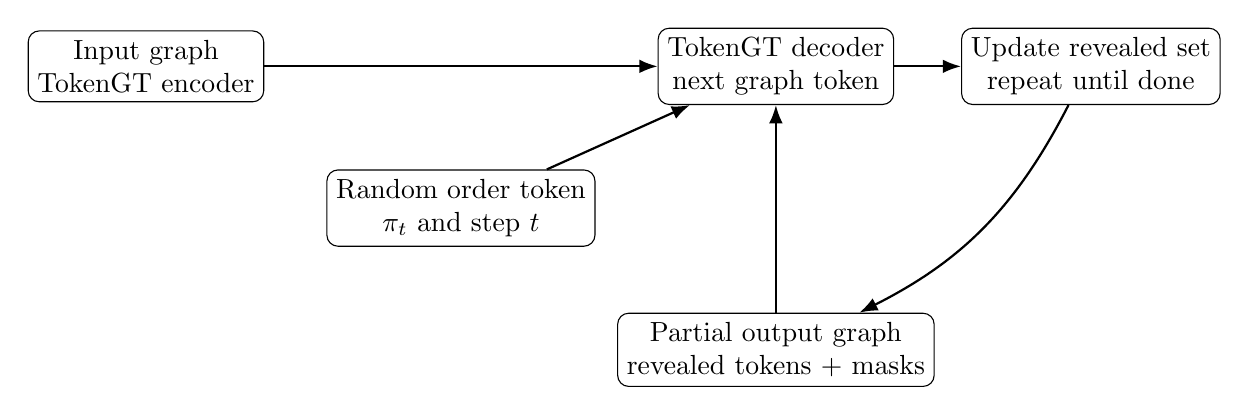
\begin{tikzpicture}[
  node/.style={draw, rounded corners, minimum width=2.4cm, minimum height=0.9cm, align=center},
  edge/.style={-Latex, thick}
]
\node[node] (enc) at (0,1.8) {Input graph\\TokenGT encoder};
\node[node] (part) at (8.0,-1.8) {Partial output graph\\revealed tokens + masks};
\node[node] (ord) at (4.0,0.0) {Random order token\\$\pi_t$ and step $t$};
\node[node] (dec) at (8.0,1.8) {TokenGT decoder\\next graph token};
\node[node] (upd) at (12.0,1.8) {Update revealed set\\repeat until done};

\draw[edge] (enc) -- (dec);
\draw[edge] (part) -- (dec);
\draw[edge] (ord) -- (dec);
\draw[edge] (dec) -- (upd);
\draw[edge, bend left=18] (upd) to (part);
\end{tikzpicture}
\caption{Random-order autoregressive graph decoding with TokenGT-style tokens.
The decoder conditions on the input graph, the currently revealed output subgraph, and the sampled decoding order rather than on a fixed left-to-right serialization.}
\label{fig:tokengt-random-order}
\end{figure}

\begin{theorem}[Universality of random-order autoregressive TokenGT decoding]
\label{thm:random-order-universality}
Fix a compact family of input graphs and a compact padded output-token space.
Assume that for every order $\pi$ and every step $t$, the target conditional law
\[
(G, y_{\pi_1},\dots,y_{\pi_{t-1}}, \pi) \mapsto
p^\star\!\bigl(y_{\pi_t}\mid G,y_{\pi_1},\dots,y_{\pi_{t-1}},\pi\bigr)
\]
is continuous in the continuous arguments.
Then for every $\varepsilon>0$ there exists a TokenGT-style random-order decoder such that the induced joint law over output graphs is within $\varepsilon$ of the target law in total variation on the compact family.
\end{theorem}

\begin{proof}
Fix an order $\pi$.
For each time step $t$, the conditional distribution is a continuous graph-to-token map on a compact domain consisting of the input graph tokenization, the partially revealed output graph, and the order embedding.
By \cref{thm:tokengt-graph-uap,cor:tokengt-graph-uap-general}, a TokenGT-style transformer can approximate each such conditional arbitrarily well.
Because the output horizon $L$ is finite, the chain rule factorization shows that the joint distribution error is controlled by the sum of per-step approximation errors.
Choosing each step error below $\varepsilon/L$ yields a total variation error below $\varepsilon$ for the fixed order.
Averaging over the order distribution $\Pi$ preserves the bound because convex combinations cannot increase total variation distance.
\end{proof}

\paragraph{Why random order matters here.}
This decoding scheme is especially relevant to the current manuscript for three reasons.
\begin{enumerate}[leftmargin=2em]
\item \textbf{Symmetry.} It respects the fact that graph outputs do not possess a privileged linear order.
\item \textbf{Compatibility with graph-valued sinks.} It lets sink decoders emit graph objects directly while keeping all intermediate reasoning in embedding space.
\item \textbf{Design flexibility.} Different orders correspond to different quiver policies; one can favor uncertain nodes first, biologically important residues first, or coarse-to-fine graph refinement.
\end{enumerate}

\paragraph{Connection to the broader theory.}
Theorem \ref{thm:tokengt-graph-uap} upgrades the transformer discussion from sequence universality to graph universality.
Theorem \ref{thm:random-order-universality} shows that graph-valued generation can be handled by boundary-aware TokenGT decoders without sacrificing universality.
Together, they justify treating graph-valued modules, graph-valued thought states, and graph-valued decoders as native citizens of the tropical quiver framework rather than as special cases bolted on afterward.

\subsection{Algebraic linguistics, graph grammars, and representational scope}
\label{sec:algebraic-linguistics}

Recent work of Marcolli, Berwick, and Chomsky develops a Hopf-algebraic description of Merge, Minimalism, and the syntax-semantics interface \cite{MarcolliChomskyBerwickMerge2023,MarcolliBerwickChomskyMinimalism2023,MarcolliBerwickChomskySyntaxSemantics2023}.
In parallel, Marcolli and Port show that graph grammars provide a mathematically rich language-theoretic formalism linked to insertion Lie algebras and quantum-field-theoretic structure \cite{MarcolliPortGraphGrammars2015}.
These papers are valuable because they identify algebraic invariants and rewrite structures that any sufficiently expressive language architecture should in principle be able to model.
However, the TokenGT universality results established above imply that one should not read such algebraic formalisms as evidence of an \emph{intrinsic representational incapacity} of transformer-style architectures.

\begin{proposition}[Bounded graph grammars lie within TokenGT representational scope]
\label{prop:graph-grammar-representability}
Let $\Gamma$ be a finite attributed graph grammar whose sentential forms lie in a compact padded family of graphs with uniformly bounded numbers of nodes and edges.
Fix either a finite derivation horizon $H$ or a canonical boundary rule for selecting a normal form.
Let
\[
F_{\Gamma}:
\mc{G}_{n_{\max},m_{\max}}^{\mathrm{in}}
\to
\mc{G}_{\bar n,\bar m}^{\mathrm{out}}
\]
denote the induced graph-to-graph transduction taking an input sentential form to the output graph obtained by applying the grammar under that bounded protocol.
Then $F_{\Gamma}$ lies in the approximation class of \cref{thm:tokengt-graph-uap,cor:tokengt-graph-uap-general}.
In particular, TokenGT-style transformers can approximate the graph-grammar transduction arbitrarily well on the compact family, and under tropicalization the local rewrite operators become chartwise piecewise-affine or max-plus maps on occupied activation regions.
\end{proposition}

\begin{proof}
Under the bounded-size and bounded-horizon assumptions, the set of admissible sentential forms is finite when labels are discrete and compact when continuous graph attributes are included.
The grammar therefore induces a well-defined graph-to-graph map on a compact padded domain.
If the transduction is equivariant with respect to graph relabeling, \cref{thm:tokengt-graph-uap} applies directly after TokenGT tokenization.
If the grammar uses a canonical derivation order, root choice, or boundary-selected normal form, \cref{cor:tokengt-graph-uap-general} applies instead.
For the tropical statement, fix a local activation chart and a local rewrite pattern; within that chart the relevant attention, projection, and feed-forward components are piecewise affine, so the induced rewrite operator is likewise chartwise piecewise affine and admits a tropical/max-plus description on the occupied region.
\end{proof}

\paragraph{What this does and does not show.}
\Cref{prop:graph-grammar-representability} does \emph{not} show that a transformer automatically discovers the correct grammar from realistic data, nor that it matches human acquisition biases, grounding, or out-of-support generalization.
Those remain difficult questions about inductive bias, optimization, and semantics.
What it \emph{does} show is narrower but still important:
if one interprets the Hopf-algebraic and graph-grammar viewpoint of \cite{MarcolliChomskyBerwickMerge2023,MarcolliBerwickChomskyMinimalism2023,MarcolliBerwickChomskySyntaxSemantics2023} as implying that transformer architectures are \emph{in principle} unable to internalize graph-grammar structure, then that interpretation is too strong.
The universality results above place bounded graph grammars and their associated algebraic transductions squarely inside the representational envelope of TokenGT-style transformers and, a fortiori, inside the tropical-quiver architectures studied in this manuscript.

\paragraph{Relevance to the present manuscript.}
This clarification matters because our quiver framework treats internal reasoning states, parse states, and multimodal world models as graph-valued embedding objects rather than as flat token strings.
In that setting, algebraic linguistics is best viewed not as a competing impossibility argument but as a source of structured priors, conserved quantities, and grammar-valued supervision signals.
The tropical perspective sharpens this point further:
graph-grammar rules act locally, quiver composition globalizes them, and tropicalization organizes the resulting dynamics into charts where one can inspect rewrite choices, stability, and compositionality directly.

\paragraph{OOD strengthening via recursive latent reasoning.}
The preceding discussion is representational.
For out-of-distribution generalization, one would like additional evidence that transformer-style systems can \emph{use} the relevant graph-structured representations in a systematically compositional way, rather than merely encode them in principle.
Recent work by Altabaa, Chen, Lafferty, and Yang provides exactly this kind of evidence: on a computational-graph reasoning task, they report robust OOD algorithmic generalization from transformers equipped with input-adaptive recurrence, algorithmic supervision, anchored latent representations through a discrete bottleneck, and explicit error-correction \cite{AltabaaChenLaffertyYang2025}.
In the language of the present manuscript, these are naturally interpreted as cyclic quiver execution, supervision on intermediate graph-valued states, boundary-compatible chart anchoring, and corrective feedback loops. This, significantly strengthen the positive case: the tropical-quiver perspective is not only broad enough to represent graph-grammar computations, but is also architecturally aligned with a class of recursive latent transformer systems that already exhibit nontrivial OOD generalization on graph-structured reasoning problems.

\newpage

\section{Path-algebra view of composable architectures}
\label{sec:path-algebra}

A quiver provides more than a bookkeeping device: it induces an algebra of compositions that mirrors how modular systems are implemented and trained.

\subsection{Paths as program traces}
A directed path $p$ in $Q$ is a sequence of edges
$p=(e_1,\dots,e_k)$ with $\tgt(e_j)=\src(e_{j+1})$.
Given a path from $u$ to $v$, the associated \emph{connector composition} is
\[
P_p := P_{e_k}\circ \cdots \circ P_{e_1},
\]
which is linear/affine if each $P_e$ is.
When modules are included, a path alternates nonlinear and linear operators.
For clarity, consider a simple chain $u\to v\to w$:
\[
y_w = N_w\!\Big(P_{v\to w}\big( N_v(P_{u\to v}(y_u))\big)\Big).
\]
In a modular system, many such paths coexist and their outputs are merged by addition, concatenation, or attention.
The \emph{set of active paths} is therefore a first-class architectural choice.

\subsection{Linear path category and path algebra (linear skeleton)}
\label{sec:linear-path-category}

The classical quiver toolbox is fundamentally \emph{linear}: it studies vector spaces attached to vertices and linear maps attached to arrows, up to changes of basis.
Our decorated quiver is nonlinear at vertices, so to access quiver theory we make this linear structure explicit via \emph{linear categories} and \emph{linearizations}.

\paragraph{Path category and its $\Bbbk$-linearization.}
The quiver $Q$ determines a small \emph{path category} $\mathrm{Path}(Q)$:
objects are vertices, a morphism $u\to v$ is a directed path $p:u\leadsto v$, and composition is path concatenation.
Its $\Bbbk$-linearization $\Bbbk\mathrm{Path}(Q)$ (a \emph{$\Bbbk$-linear category}) has the same objects and
\[
\mathrm{Hom}_{\Bbbk\mathrm{Path}(Q)}(u,v) := \mathrm{span}_{\Bbbk}\{p:u\leadsto v\},
\]
with bilinear composition.
This is the minimal ``linear category'' associated with a quiver: it turns discrete paths into a linear basis while preserving composition.

\paragraph{Path algebra.}
Fix a field $\Bbbk$ (in practice $\R$).
The \emph{path algebra} $\Bbbk Q$ is the $\Bbbk$-vector space with basis all directed paths (including length-zero idempotents at each vertex), with multiplication given by path concatenation when composable and $0$ otherwise.
Equivalently, $\Bbbk Q$ is the endomorphism algebra of the direct sum of objects in the $\Bbbk$-linear path category.

We use $\Bbbk Q$ in a deliberately restricted way:
\begin{itemize}[leftmargin=2em]
\item It provides a language for \emph{routing}: selecting paths corresponds to selecting basis elements.
\item It supports \emph{parameter tying} and \emph{relations}: equalities between path compositions correspond to quotienting by an ideal of relations.
\item It suggests \emph{algebraic regularizers}: penalize commutators or enforce approximate relations between compositions that should be equivalent by design.
\end{itemize}

\paragraph{Quiver representations as executable linear programs.}
A finite-dimensional \emph{(linear) representation} of $Q$ assigns to each vertex $v$ a vector space $E_v$ and to each edge $e:u\to v$ a linear map $A_e:E_u\to E_v$.
Two representations are equivalent if they differ only by a change of basis in each $E_v$.
This is precisely the setting where the full quiver toolbox applies: classification by invariants, path-algebra modules, and gauge-style consistency around cycles.
(Equivalently: a representation is a $\Bbbk$-linear functor $\Bbbk\mathrm{Path}(Q)\to\mathrm{Vect}$.)

\paragraph{Linearizing nonlinear vertices and keeping the linearization \emph{at vertices}.}
The classical quiver toolbox assumes a linear assignment: vector spaces at vertices and linear maps on arrows.
Our decorated quiver is nonlinear at vertices, so to access quiver theory we explicitly factor the local linearization into
\emph{(a) connector linear maps on edges} and \emph{(b) Jacobian blocks on vertices}.

Fix an execution state (a DAG input, an unrolled time index, or a fixed point of a cyclic SCC).
Write $(x_v^{(1)},\dots,x_v^{(m_v)})$ for the current inputs to $N_v$ and $y_v:=N_v(x_v)$ for its output.
Define tangent spaces
\[
T^{\text{out}}_v := T_{y_v}Y_v\cong \R^{d^{\text{out}}_v},
\qquad
T^{\text{in}}_{v,i} := T_{x_v^{(i)}}\Emb_{\alpha_i(v)}\cong \R^{d^{\text{in}}_{v,i}}.
\]
For a module $N_v:X_v\to Y_v$ with input ports $(x_v^{(1)},\dots,x_v^{(m_v)})$, let
\[
J_{v,i} := \frac{\partial N_v}{\partial x_v^{(i)}}\Big|_{x_v}
\;:\; T^{\text{in}}_{v,i}\to T^{\text{out}}_v
\]
denote the partial Jacobian block evaluated at the current state.
For an edge $e:u\to v$ landing in port $i(e)$, write the connector as $P_e(z)=A_e z+b_e$ and keep only its linear part $A_e$ in the linearization.

The resulting first-order perturbation dynamics factor cleanly:
\begin{align}
\delta x_v^{(i)} &= \sum_{e\in \mathrm{In}(v):\, i(e)=i} A_e\,\delta y_{\src(e)},
\label{eq:lin-message-in}
\\
\delta y_v &= \sum_{i=1}^{m_v} J_{v,i}\,\delta x_v^{(i)}.
\label{eq:lin-message-out}
\end{align}
Equations \eqref{eq:lin-message-in}--\eqref{eq:lin-message-out} are the exact content we want quiver theory to ``see'':
all nonlinearities are summarized by Jacobian blocks that live \emph{at the vertex} (one block per input port). If it helps the reader coming from quiver theory, one may think of linearized vertices as loops at the vertex. 

\paragraph{Port-expanded linearization quiver.}
To represent \eqref{eq:lin-message-in}--\eqref{eq:lin-message-out} as an ordinary quiver representation, we expand the graph so that each input port becomes its own vertex.
Define the \emph{linearization quiver} $Q^{\mathrm{lin}}$ with vertices
\[
\Nodes^{\mathrm{lin}} := \{v^{\text{out}}:v\in\Nodes\}\ \cup\ \{(v,i)^{\text{in}}: v\in\Nodes,\ i\in\{1,\dots,m_v\}\},
\]
and arrows of two types:
\begin{itemize}[leftmargin=2em]
\item \textbf{Connector arrows:} for each original edge $e:u\to v$ landing in port $i(e)$, an arrow
$(u^{\text{out}}\to (v,i(e))^{\text{in}})$ labeled by $A_e$.
\item \textbf{Module Jacobian arrows:} for each module $v$ and each port $i$, an internal arrow
$((v,i)^{\text{in}}\to v^{\text{out}})$ labeled by $J_{v,i}$.
\end{itemize}
Assign vector spaces $E_{v^{\text{out}}}:=T^{\text{out}}_v$ and $E_{(v,i)^{\text{in}}}:=T^{\text{in}}_{v,i}$.
Then $(\{E_w\}_{w\in\Nodes^{\mathrm{lin}}},\{A_a\}_{a\in\Edges^{\mathrm{lin}}})$ is a standard finite-dimensional quiver representation, to which the full linear quiver toolbox applies.

\begin{definition}[Port-expanded Jacobian representation]
Fix an execution state.
The associated \emph{port-expanded Jacobian representation} is the representation
\[
\mc{R}^{\mathrm{port}}_{\mathrm{Jac}} := (\{E_w\}_{w\in\Nodes^{\mathrm{lin}}},\{A_a\}_{a\in\Edges^{\mathrm{lin}}}),
\]
where $E_{v^{\text{out}}}=T^{\text{out}}_v$, $E_{(v,i)^{\text{in}}}=T^{\text{in}}_{v,i}$, connector arrows carry $A_e$, and module arrows carry $J_{v,i}$.
\end{definition}

\paragraph{Collapsed ``output-only'' representation (derived).}
If one prefers a representation on outputs only, compose inside each target vertex to eliminate input-port nodes.
This yields effective edge maps
\begin{equation}
A_e^{\mathrm{eff}} := J_{\tgt(e),i(e)}\,A_e : T^{\text{out}}_{\src(e)}\to T^{\text{out}}_{\tgt(e)}.
\label{eq:linearized-edge}
\end{equation}
The resulting output-only representation is convenient for cycle spectra, but the port-expanded view keeps vertex linearizations explicit and is the correct object for diagnosing \emph{which port/block} creates instability.

\begin{remark}[Almost-everywhere differentiability]
For piecewise-smooth modules (ReLU, max, attention with softmax, etc.), Jacobians exist almost everywhere.
In implementation one uses automatic differentiation with a consistent subgradient convention.
All diagnostics built from $J_{v,i}$, $A_e$, or the collapsed maps $A_e^{\mathrm{eff}}$ are therefore well-defined for almost all minibatch states.
\end{remark}

Along a path in $Q^{\mathrm{lin}}$, linear maps are ordinary matrix products alternating $A_e$ and $J_{v,i}$.
Along a directed cycle, the resulting composite is square; its spectrum directly controls local stability and gradient amplification.

\paragraph{Translating linear analysis back to nonlinear learning.}
The Jacobian blocks $J_{v,i}$ and connector linear parts $A_e$ are extracted from the current nonlinear execution and used for \emph{diagnostics and regularization}.
All of the resulting quantities are differentiable with respect to model parameters:
one can backpropagate through Jacobian--vector products (JVPs) or vector--Jacobian products (VJPs) without explicitly materializing full Jacobian matrices.
Consequently, penalties based on (i) cycle spectral radii, (ii) commutator norms, (iii) holonomy/curvature surrogates, or (iv) port-local instability scores can be trained end-to-end.
The forward computation remains entirely in embedding space; no intermediate discretization is required.

\paragraph{Tropical cellwise dynamics as a global combinatorial representation.}
For a cyclic subgraph defining dynamics $z_{t+1}=\Psi(z_t)$ on state space $Z$, tropical geometry yields an activation fan, a cellwise affine representation, and max-plus cocycles that are exact for piecewise-linear modules and locally accurate for smooth modules after tropicalization.
With a learned observable encoder $\psi_\eta:Z\to\R^d$ and a fitted matrix $K$ satisfying $\psi_\eta(z_{t+1})\approx K\psi_\eta(z_t)$, powers of $K$ approximate multi-step evolution.
This provides a complementary linear representation of the cycle \emph{semigroup} that captures global behavior beyond local Jacobians (developed in \cref{sec:tropical-cycle-dynamics}).

\subsection{Nonlinear path operators and mixture-of-paths}

To incorporate nonlinear modules, define for any path that visits vertices $v_1\to v_2\to\cdots\to v_k$ the \emph{path operator}
\[
\mc{T}_p := N_{v_k}\circ P_{e_{k-1}}\circ N_{v_{k-1}}\circ \cdots \circ P_{e_1}\circ N_{v_1}.
\]
These operators do not form an algebra under addition/composition in general, but two implementable patterns recover a useful ``algebra-like'' structure.

\paragraph{(1) Gated path sums (mixture-of-paths).}
Let $\mc{P}(u\to v)$ be a set of candidate paths from $u$ to $v$.
Define an output as a convex or learned mixture
\[
y_v = \sum_{p\in \mc{P}(u\to v)} \pi_p(x)\,\mc{T}_p(x),
\qquad \pi_p(x)\ge 0,\ \sum_p \pi_p(x)=1.
\]
This expresses mixture-of-experts, ensemble routing, and tool selection graphs as \emph{mixture-of-paths}.
Importantly, $\pi_p$ can be computed by a router module that itself is a vertex in the quiver.

\paragraph{(2) Linearization in a feature space.}
For cyclic graphs or stability analysis, we often linearize around a trajectory.
The Jacobian of each module yields linear operators that \emph{do} compose in a path algebra, enabling computable bounds on contraction and spectral radii.
This is one bridge between deep learning practice (Jacobian diagnostics) and operator algebra (\cref{sec:operator-algebra}).

\subsection{Relations and ``interfaces as contracts''}
Many modular systems rely on equivalences:
two different subgraphs are expected to compute the same representation (up to a connector), or a bypass path should be functionally close to a main path (distillation).
We encode such assumptions as \emph{relations}:
\[
\mc{T}_{p_1}(x) \approx \mc{T}_{p_2}(x) \quad\text{for relevant }x.
\]
Relations are enforced by distillation losses and, when linear connectors dominate, by operator-algebraic penalties on compositions.
This yields an implementable ``interface contract'' view:
\begin{itemize}[leftmargin=2em]
\item each port has a type and shape,
\item each connector defines a differentiable map between port spaces,
\item relations specify which composed maps should agree.
\end{itemize}

\subsection{Practical implication: composability favors explicit connector modules}
A recurring engineering failure mode is to hide complex transforms inside edges or ad hoc tensor reshapes.
Within our formalism, the recommended pattern is:
\emph{if an interface needs nontrivial nonlinear processing (attention, normalization, alignment with context), represent it as an explicit module vertex with its own ports and diagnostics}.
Edges remain simple (linear/affine), making them cheap to search over and easy to regularize.

\newpage

\section{Operator-algebra structure of modular graphs}
\label{sec:operator-algebra}

Operator-algebra language is useful when it produces \emph{computable} and \emph{actionable} quantities: norms, spectra, commutators, and stability margins.
We therefore keep the discussion tied to implementation.

\subsection{Two linear operator lifts}
There are two complementary ways to associate linear operators to a nonlinear decorated quiver.

\paragraph{(A) Linearization on embedding spaces.}
Fix an execution mode (DAG evaluation, unrolled cycles, or a fixed point) and consider the input--output map implemented by the whole graph,
$F_{\theta,P}: \mc{X}\to \mc{Y}$, where $\mc{X}$ and $\mc{Y}$ are products of typed spaces.
For a particular input $x$ (or state $z^\star$), the Jacobian $J_F(x)$ is a linear map on the tangent space.
At the module level, each $N_v$ has a Jacobian $J_{N_v}$; connectors already are linear/affine.
Compositions of these Jacobians along paths form a noncommutative algebra of linear maps that directly controls stability and gradient behavior.

\paragraph{(B) Tropical lift on activation fans.}
For cyclic subgraphs defining dynamics $z_{t+1}=\Psi(z_t)$, the activation fan together with cellwise affine data $(A_C,b_C)$ provides a combinatorial lift that preserves switching structure and supports max-plus cocycles on itineraries.
This lift can capture global nonlinear behavior beyond local Jacobians.
We develop this in depth in \cref{sec:tropical-cycle-dynamics}.

Both lifts generate algebras under composition; (A) is local and directly computable by autodiff; (B) is global and data-driven.

\subsection{Generated algebras and commutator diagnostics}
Let $\mc{H}$ be a Hilbert space representing a chosen embedding space or observable space.
Consider a set of bounded linear operators $\{T_i\}\subset \mc{B}(\mc{H})$ (e.g., connectors, Jacobians, or cellwise affine fits extracted from a tropical model).
The (non-unital) algebra generated by $\{T_i\}$ is
\[
\mc{A}:=\mathrm{Alg}(T_1,\dots,T_m)\subseteq \mc{B}(\mc{H}),
\]
the smallest subalgebra closed under addition, scalar multiplication, and composition that contains the $T_i$.

\paragraph{Why does $\mc{A}$ matter in practice?}
Many desirable properties are about \emph{almost-commuting} operators:
\begin{itemize}[leftmargin=2em]
\item If two transformations should be order-insensitive (e.g., normalization vs. projection), enforce a small commutator $\norm{T_iT_j-T_jT_i}$.
\item If a connector should preserve a symmetry represented by a group action $S_g$, enforce $T S_g\approx S_g T$ (equivariance transfer).
\item If a cycle should be stable, enforce spectral constraints on the composite operator along the cycle.
\end{itemize}
All of these become explicit, differentiable penalties once we fix a finite-dimensional representation (embeddings, Jacobians, or tropical activation-fan models).

\subsection{Composite operators for cycles}
Let $c=(v_1\to v_2\to \cdots \to v_k \to v_1)$ be a directed cycle involving a subset of stateful vertices.
Under unrolled semantics, the cycle defines an iterated map $\Psi$ on state; under fixed-point semantics, it defines the update map $\Phi$.
In both cases, a central object is the \emph{cycle composite} operator:
\[
\Psi = \Psi_{c,\theta,P} := \pi_{v_1}\circ \mathrm{Exec}_c,
\]
where $\mathrm{Exec}_c$ denotes one pass around the cycle and $\pi_{v_1}$ projects back to the starting state component.
Stability is controlled by the Jacobian $D\Psi$ (local) together with tropical growth and transition structure on the activation fan (global/combinatorial).

\subsection{Operator-algebra regularizers that remain implementable}
We highlight three families of regularizers that are both meaningful and cheap enough to use.

\paragraph{(1) Norm and conditioning control.}
For each connector $P_e(z)=A_e z+b_e$, regularize $\opnorm{A_e}$ (via spectral normalization or power iteration estimates).
This caps amplification along paths and stabilizes cycles.

\paragraph{(2) Approximate commutation constraints.}
If a known linear action $S$ (e.g., permutation of tokens, rotation/reflection in equivariant models, or channel symmetries) should commute with a connector, penalize
\[
L_{\mathrm{comm}}=\sum_e \Frob{A_e S - S A_e}^2.
\]
This is a practical way to transfer equivariance between pretrained modules with mismatched internal bases.

\paragraph{(3) Spectral shaping of cyclic composites.}
For a cycle composite Jacobian $J_c$ or tropical cellwise approximant $A_C$, penalize spectral radius or enforce cellwise contraction inside a desired region:
\[
L_{\rho} = \sum_c \max(0,\rho(J_c)-\gamma)^2
\quad\text{or}\quad
L_{\mathrm{eig}}=\sum_c \sum_{i} \phi(\lambda_i(K_c)),
\]
where $\phi$ penalizes eigenvalues outside stability/mixing bands.
\Cref{sec:tropical-cycle-dynamics} details how to estimate $\lambda_i(K_c)$ in practice.

\newpage

\section{Tropical geometry for cyclic subgraphs}
\label{sec:tropical-cycle-dynamics}

Directed cycles are where modular systems most frequently fail: instability, exploding/vanishing gradients, self-reinforcing routing, or semantically meaningless feedback between misaligned representations.
Our central claim is that for such cycles the right primary language is \emph{tropical geometry plus ergodic theory}, not an externally chosen global linear lift such as those found in Koopman theory.
The reason is simple:
the nonlinearity of modern modular systems is dominated by switching between piecewise-affine contexts, and that switching is precisely what activation fans, tropical rational maps, and real tropical decision complexes describe.

\subsection{From cyclic quivers to tropical dynamical systems}
Consider a cyclic subgraph with state space
\[
Z=\prod_{v\in\Nodes_\mathrm{state}} Y_v.
\]
Fix external inputs (or treat them as exogenous signals).
Execution defines a discrete-time dynamical system
\begin{equation}
z_{t+1} = \Psi(z_t),
\label{eq:dynamics}
\end{equation}
where $\Psi$ may represent:
\begin{itemize}[leftmargin=2em]
\item one full sweep of message passing around a cycle (explicit iteration),
\item one application of the global update $\Phi$ restricted to stateful vertices,
\item a learned sampler step or refinement step parameterized by module outputs.
\end{itemize}

\begin{definition}[Tropicalized cyclic update]
We say that \eqref{eq:dynamics} is \emph{tropicalized} on a region $\Omega\subseteq Z$ if there exists a finite polyhedral fan $\Sigma_\Psi(\Omega)$ such that for each maximal cell $C\in\Sigma_\Psi(\Omega)$ the restriction $\Psi|_C$ is affine and each coordinate of $\Psi$ is representable as a tropical rational function on $\Omega$.
\end{definition}

\begin{proposition}[Exactness for piecewise-linear modular cycles]
Suppose every vertex operator in a cyclic subgraph is piecewise affine with finitely many regions and every connector is affine.
Then, after choosing Euclidean coordinates on typed ports, the induced global map $\Psi$ is piecewise affine and coordinatewise tropical rational.
In particular, its state space admits a finite activation fan $\Sigma_\Psi$ whose cells are maximal regions of affine execution.
\end{proposition}

This is the cyclic analogue of the exact tropical description of ReLU networks in \cite{ZhangNaitzatLim2018}.
For modular quivers the fan is obtained by refining the fans of vertex operators and connectors across all ports participating in the cycle.

\paragraph{Why this is better than a global spectral lift.}
The fan $\Sigma_\Psi$ records \emph{which} affine setting is active, \emph{where} switching occurs, and \emph{which faces} generate instability.
These are precisely the pieces of information practitioners need when debugging a cyclic architecture.

\subsection{Activation fans, cellwise affine execution, and decision complexes}
Let $\Sigma_\Psi$ be the activation fan of a cyclic subgraph.
For each cell $C\in\Sigma_\Psi$ we have
\[
\Psi(z)=A_C z+b_C,\qquad z\in C,
\]
for some affine data $(A_C,b_C)$.
The boundaries between cells form a polyhedral complex of \emph{switching hypersurfaces}.
When the cycle produces a binary decision, termination flag, or gating event, the induced separating set is a real-tropical decision complex in the sense of \cite{BrandenburgLohoMontufar2024}.

\begin{definition}[Activation itinerary]
Given $z_0\in Z$, its \emph{activation itinerary} is the sequence
\[
\omega(z_0)=(C_0,C_1,C_2,\dots),\qquad C_t\in\Sigma_\Psi,\ z_t\in C_t.
\]
\end{definition}

This converts cyclic execution into a symbolic process on a finite or countable state space of cells.
The geometry of the cycle is therefore encoded simultaneously by:
\begin{enumerate}[leftmargin=2em]
\item the cellwise affine data $(A_C,b_C)$,
\item the adjacency/transition structure of the fan,
\item the real-tropical decision subcomplexes where semantics or routing change.
\end{enumerate}

\paragraph{Interpretation for quivers.}
In a quiver, a ``bad loop'' may arise because:
(i) a connector holonomy is inconsistent;
(ii) a local affine map expands too much on some cells; or
(iii) trajectories repeatedly skim switching hypersurfaces.
Tropical geometry separates these mechanisms.

\begin{figure}[t]
\centering
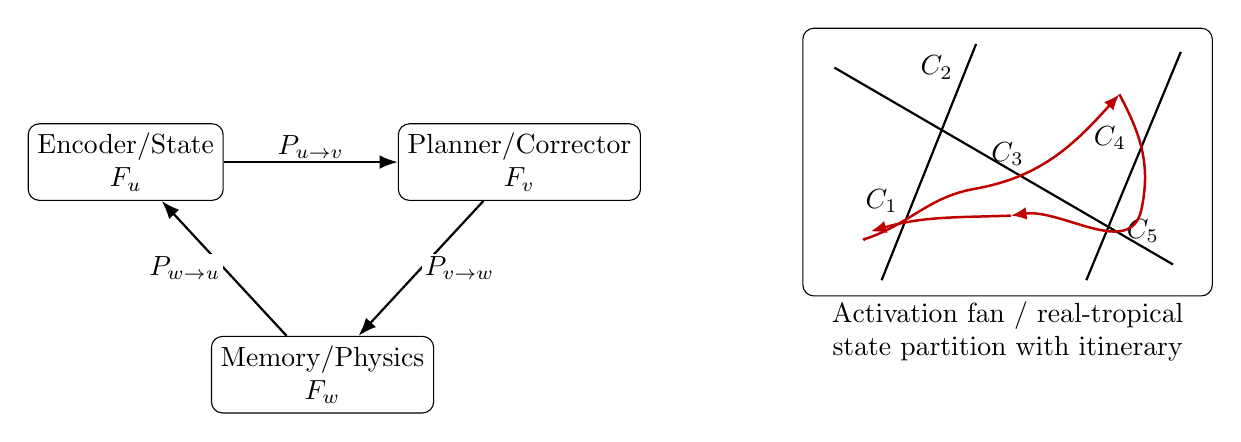
\begin{tikzpicture}[
  qnode/.style={draw, rounded corners, minimum width=2.2cm, minimum height=0.9cm, align=center},
  edge/.style={-Latex, thick},
  cellline/.style={thick},
  lab/.style={fill=white, inner sep=1pt},
  traj/.style={red!75!black, line width=0.9pt, -{Latex[length=2.0mm,width=1.6mm]}}
]
% Quiver on the left
\node[qnode] (A) at (-1.0,1.7) {Encoder/State\\$F_u$};
\node[qnode] (B) at (4.0,1.7) {Planner/Corrector\\$F_v$};
\node[qnode] (C) at (1.5,-1.0) {Memory/Physics\\$F_w$};
\draw[edge] (A) -- node[lab, above] {$P_{u\to v}$} (B);
\draw[edge] (B) -- node[lab, right] {$P_{v\to w}$} (C);
\draw[edge] (C) -- node[lab, left] {$P_{w\to u}$} (A);

% State-space partition on the right
\begin{scope}[xshift=7.6cm]
  \draw[rounded corners] (0,0) rectangle (5.2,3.4);
  \draw[cellline] (1.0,0.2) -- (2.2,3.2);
  \draw[cellline] (0.4,2.9) -- (4.7,0.4);
  \draw[cellline] (3.6,0.2) -- (4.8,3.1);
  \node at (1.0,1.2) {$C_1$};
  \node at (1.7,2.9) {$C_2$};
  \node at (2.60,1.80) {$C_3$};
  \node at (3.9,2.0) {$C_4$};
  \node at (4.32,0.82) {$C_5$};
  \draw[traj] (0.78,0.72) to[out=18,in=190] (2.18,1.36) to[out=10,in=228] (4.02,2.56);
  \draw[traj] (4.02,2.56) to[out=298,in=78] (4.30,1.10) to[out=258,in=8] (2.64,1.02);
  \draw[traj] (2.64,1.02) to[out=182,in=16] (0.86,0.82);
  \fill[red!75!black] (0.78,0.72) circle (0.7pt);
  \node[align=center] at (2.6,-0.45) {Activation fan / real-tropical\\state partition with itinerary};
\end{scope}
\end{tikzpicture}
\caption{Left: a cyclic decorated quiver with three interacting modules. Right: the induced activation fan on a low-dimensional state slice. The red trajectory depicts the sample activation itinerary $C_1\to C_3\to C_4\to C_5\to C_4\to C_1$; instability may arise from an expanding cell, a sticky subfan, or repeated grazing of switching boundaries.}
\label{fig:tropical-cycle-fan}
\end{figure}

\subsection{Ergodic activation itineraries, invariant measures, and mixing}
\label{sec:ergodic}

The correct measure-theoretic object is the pair consisting of an invariant measure on $Z$ and the induced stationary process on activation itineraries.

\begin{definition}[Invariant measure]
A probability measure $\mu$ on $Z$ is \emph{invariant} for $\Psi$ if $\mu(\Psi^{-1}(A))=\mu(A)$ for all measurable $A\subseteq Z$.
\end{definition}

\begin{definition}[Ergodicity and mixing (practical)]
The dynamical system $(Z,\Psi,\mu)$ is \emph{ergodic} if every $\Psi$-invariant set has $\mu$-measure $0$ or $1$.
It is \emph{(strong) mixing} if for any $f,g\in L^2(\mu)$,
\[
\mathrm{Cov}\bigl(f\circ \Psi^t,\, g\bigr)\to 0
\qquad\text{as }t\to\infty.
\]
\end{definition}

Ergodicity implies that \emph{time averages along one typical trajectory} recover expectations under $\mu$; mixing controls \emph{how many steps} we need for effectively independent samples.
This remains true whether $f$ is a connector norm, a holonomy residual, a Hodge energy, a cell label indicator, or a tropical potential.

\begin{theorem}[Birkhoff ergodic theorem (used here as a modeling assumption)]
If $(Z,\Psi,\mu)$ is measure-preserving and ergodic, then for any $f\in L^1(\mu)$ and for $\mu$-almost every initial state $z_0$,
\[
\frac{1}{T}\sum_{t=0}^{T-1} f(z_t)\ \longrightarrow\ \int f\,\mathrm{d}\mu,
\qquad z_{t+1}=\Psi(z_t).
\]
\end{theorem}

See \cite{WaltersErgodic} for standard statements and variants.

\paragraph{Why this matters for tropical diagnostics.}
If the cycle is not approximately stationary and ergodic on the timescale of data collection, then any fitted tropical model reflects transient drift rather than the long-run loop.
We therefore recommend logging stationarity checks, boundary-hit rates, and an \emph{integrated autocorrelation time} estimate to size trajectory windows.

\begin{algorithm}[t]
\caption{Ergodic diagnostics for a cyclic subgraph (effective sample size)}
\label{alg:ergodic}
\begin{algorithmic}[1]
\Require trajectory $(z_t)_{t=0}^{T}$, scalar observable $f(z)$, max lag $L$
\State compute $f_t \gets f(z_t)$ and center $f_t \gets f_t - \frac{1}{T+1}\sum_{t=0}^{T} f_t$
\State estimate autocorrelation $\hat\rho(\ell)=\frac{\sum_{t=0}^{T-\ell} f_t f_{t+\ell}}{\sum_{t=0}^{T} f_t^2}$ for $\ell=1,\dots,L$
\State integrated autocorrelation time $\widehat{\tau}_{\mathrm{int}} \gets 1 + 2\sum_{\ell=1}^{L} \max(0,\hat\rho(\ell))$
\State effective sample size $\widehat{N}_{\mathrm{eff}} \gets \frac{T+1}{\widehat{\tau}_{\mathrm{int}}}$
\State \Return $(\widehat{\tau}_{\mathrm{int}}, \widehat{N}_{\mathrm{eff}})$
\end{algorithmic}
\end{algorithm}

\paragraph{Ergodicity of cycle-space observables.}
Holonomy, curvature surrogates, Hodge energies, activation-cell indicators, and tropical potentials are all observables $f(z_t)$ evaluated along the execution trajectory.
Under ergodicity they have well-defined long-run averages; under poor mixing they drift or lock into ``circular'' attractors, which is precisely the failure mode we want to detect.

\subsection{Max-plus cocycles and tropical growth rates}
The key long-run growth diagnostic is a \emph{max-plus cocycle growth rate} attached to the activation itinerary.

\begin{definition}[Tropical cocycle]
To each occupied cell $C\in\Sigma_\Psi$ attach a max-plus matrix $M_C$ encoding dominant affine gains, routing costs, or log-amplification scores.
Along an activation itinerary $\omega=(C_0,C_1,\dots)$ define the cocycle product
\[
\Gamma_T(\omega)=M_{C_{T-1}}\otimes \cdots \otimes M_{C_0},
\]
where $\otimes$ denotes max-plus matrix multiplication.
\end{definition}

The choice of $M_C$ is application dependent.
For stability diagnostics, a practical choice is
\[
(M_C)_{ij}=\log\!\bigl(\varepsilon + |(A_C)_{ij}|\bigr),
\]
possibly augmented by connector or resource penalties on edges.

\begin{theorem}[Tropical growth rate via subadditivity]
\label{thm:tropical-growth}
Assume the itinerary process $(C_t)$ is stationary and ergodic and that
\[
\E\bigl[\max(0,\max_{ij}(M_{C_0})_{ij})\bigr] < \infty.
\]
Then the limit
\[
\chi_{\mathrm{trop}}
\;:=\;
\lim_{T\to\infty}\frac{1}{T}\max_{i,j}\bigl(\Gamma_T(\omega)\bigr)_{ij}
\]
exists almost surely and in $L^1$.
\end{theorem}

\begin{proof}[Proof sketch]
Set $a_T(\omega)=\max_{i,j}(\Gamma_T(\omega))_{ij}$.
The max-plus product implies $a_{T+S}(\omega)\le a_T(\omega)+a_S(\sigma^T\omega)$, so $(a_T)$ is subadditive over the shift $\sigma$ on itineraries.
Apply Kingman's subadditive ergodic theorem \cite{KingmanSubadditive}.
\end{proof}

\paragraph{Interpretation.}
\begin{itemize}[leftmargin=2em]
\item $\chi_{\mathrm{trop}}<0$ indicates average contraction in the chosen logarithmic scale.
\item $\chi_{\mathrm{trop}}\approx 0$ indicates a slow mode, neutral loop, or metastable memory.
\item $\chi_{\mathrm{trop}}>0$ indicates expanding/circular behavior and should trigger intervention.
\end{itemize}

\paragraph{Cellwise growth descriptors.}
The diagnostic triple is now:
\begin{enumerate}[leftmargin=2em]
\item the activation transition kernel on cells,
\item the cellwise affine cocycle $(A_C,b_C)$,
\item the tropical growth rates and maximum cycle means derived from $(M_C)$.
\end{enumerate}
Unlike a single linear lift on arbitrary observables, this triple tells us \emph{where} the instability lives.

\subsection{Local tropicalization for smooth modules, neural operators, and fluid solvers}
The exact tropical picture applies to piecewise-linear modules.
For smooth operators---including neural operators, PDE correctors, and Navier--Stokes-inspired latent dynamics---we use local tropical charts.

\begin{proposition}[Local tropical charts on bounded energy shells]
Let $\Omega\subset Z$ be compact and assume $\Psi:\Omega\to Z$ is Lipschitz.
Then for every $\varepsilon>0$ there exists a piecewise-affine map $\Psi_\varepsilon$ such that
\[
\sup_{z\in\Omega}\norm{\Psi(z)-\Psi_\varepsilon(z)}\le \varepsilon.
\]
If $\Psi$ is implemented by a ReLU or residual network, $\Psi_\varepsilon$ may be taken tropical rational.
\end{proposition}

Thus the tropical program is not limited to purely combinatorial models.
For neural operators and fluid solvers one first restricts to a bounded energy shell, then studies either an exact piecewise-linear surrogate or a local fan extracted from Jacobian sign patterns and residual gates.

\subsection{Data-driven tropical estimation}
To use tropical geometry in modular ML we need estimators that operate on trajectories and module logs.
The good news is that activation fans are \emph{easier} to estimate than global spectral objects:
the relevant variables are active pieces, cell transitions, and local affine fits.

\subsubsection{Activation fan estimation}
During execution, log the active branch, gate, or affine region of each module in the cyclic subgraph.
The joint label defines an activation cell $C_t$.
Aggregating observed labels yields an empirical subfan together with a transition graph between occupied cells.

\subsubsection{Cellwise tropical regression}
For each sufficiently occupied cell $C$, fit the affine map
\[
z_{t+1}\approx A_C z_t+b_C
\qquad\text{for } z_t\in C.
\]
This is a standard least-squares problem and is considerably more stable than fitting a single global operator to all trajectories.
Boundary cells may be handled by robust regression or ignored until sufficiently populated.

\subsubsection{Learned tropical invariants}
Parameterize a tropical rational observable
\[
\varphi_\eta(z)=g_\eta(z)-h_\eta(z),
\]
with $g_\eta,h_\eta$ convex piecewise-linear functions (or max-affine layers).
Train it so that $\varphi_\eta(z_{t+1})\approx \varphi_\eta(z_t)$ on trajectories.
Because the model class already matches the geometry of the dynamics, these invariants are interpretable cellwise and can often be pushed through graph rewrites more reliably than arbitrary latent features.

\begin{algorithm}[t]
\caption{Activation-fan and tropical-cocycle diagnostics for a cyclic subgraph}
\label{alg:tropical-cocycle}
\begin{algorithmic}[1]
\Require trajectory $(z_t)_{t=0}^{T}$, logged activation labels $(C_t)$, minimum cell count $m$
\State build empirical transition counts $N_{CD}=\#\{t: C_t=C,\ C_{t+1}=D\}$ and kernel $\widehat P(D\mid C)$
\For{each occupied cell $C$ with count at least $m$}
  \State fit $z_{t+1}\approx A_C z_t+b_C$ using snapshots with $z_t\in C$
  \State form max-plus weight matrix $(M_C)_{ij}\gets \log(\varepsilon + |(A_C)_{ij}|)$
\EndFor
\State estimate effective sample size via \cref{alg:ergodic} on selected observables
\State estimate tropical growth by long products $\Gamma_T=M_{C_{T-1}}\otimes\cdots\otimes M_{C_0}$
\State optionally compute maximum cycle mean on the occupied transition graph
\State \Return empirical fan, transition kernel, local affine fits, tropical growth diagnostics
\end{algorithmic}
\end{algorithm}

\subsection{Tropical-guided stability and design of cycles}
Tropical diagnostics provide actionable signals for cycle design.

\paragraph{Stability.}
For deterministic cycles, contractive behavior corresponds to:
\begin{enumerate}[leftmargin=2em]
\item $\rho(D\Psi(z^\star))<1$ near relevant fixed points,
\item negative or sufficiently small tropical growth $\chi_{\mathrm{trop}}$,
\item low boundary-hit rates, i.e. trajectories do not bounce chaotically across switching hypersurfaces.
\end{enumerate}

it is important to note here, under GFlowNets training, exploratory switching behavior with reward proportional to a distribution is expected and desirable when training embedding space GoT reasoning models, and should be tunable based on the tropical trajectories and their statistics. 

\paragraph{Mixing.}
For sampling-style cycles, rapid mixing corresponds to:
\begin{enumerate}[leftmargin=2em]
\item short integrated autocorrelation times,
\item broad occupation of activation cells,
\item a transition graph without nearly absorbing subfans unless such memory is intended.
\end{enumerate}

\paragraph{Learnable invariants as interface checks.}
If two modules participate in a cycle implementing a physical or algorithmic invariant (mass conservation, energy, normalization, conservation of a latent PDE quantity), a learned tropical invariant $\varphi_\eta$ should remain stable.
Deviation indicates interface mismatch or unstable feedback.

\paragraph{Decision-boundary localization.}
The real-tropical boundary complex tells us exactly where the cycle changes combinatorial paradigms.
Monitoring how often trajectories approach or cross this complex turns ``the loop feels brittle'' into a measurable quantity.


\begin{figure}[t]
\centering
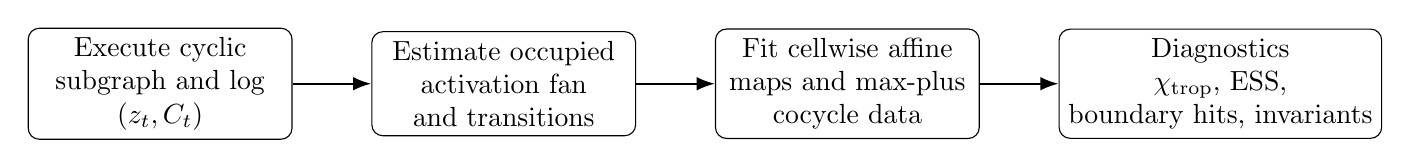
\begin{tikzpicture}[
  box/.style={draw, rounded corners, minimum width=3.35cm, minimum height=0.9cm, align=center},
  edge/.style={-Latex, thick}
]
\node[box] (traj) {Execute cyclic\\subgraph and log\\$(z_t,C_t)$};
\node[box, right=1.0cm of traj] (fan) {Estimate occupied\\activation fan\\and transitions};
\node[box, right=1.0cm of fan] (fit) {Fit cellwise affine\\maps and max-plus\\cocycle data};
\node[box, right=1.0cm of fit] (diag) {Diagnostics\\$\chi_{\mathrm{trop}}$, ESS,\\boundary hits, invariants};

\draw[edge] (traj) -- (fan);
\draw[edge] (fan) -- (fit);
\draw[edge] (fit) -- (diag);
\end{tikzpicture}
\caption{Tropical diagnostics pipeline: Practical tropical workflow for cyclic quiver subgraphs. The key step is to preserve activation-cell information rather than collapsing all trajectories into one global linear fit.}
\label{fig:tropical-pipeline}
\end{figure}

\subsection{Integration with training}
Tropical quantities can be used in three ways:
\begin{enumerate}[leftmargin=2em]
\item \textbf{Offline diagnostics:} periodically estimate occupied activation fans and tropical cocycles on held-out trajectories and flag unstable cycles.
\item \textbf{Online regularizers:} add differentiable penalties based on boundary-hit rates, cellwise contraction defects, or tropical-invariance prediction errors.
\item \textbf{Learned tropical invariants:} train $\varphi_\eta(z)=g_\eta(z)-h_\eta(z)$ such that $\varphi_\eta(\Psi(z))\approx \varphi_\eta(z)$ and use it as a constraint or a shaping reward in graph search.
\end{enumerate}

We return to the invariant toolbox in \cref{sec:invariants} and to implementation details in \cref{app:tropical-estimation}.

\subsection{Research directions at the tropical--dynamical interface}
\label{sec:tropical-research-directions}

The interaction between tropical geometry, dynamics, and ergodic theory is still underdeveloped for modern learned systems.
The quiver formalism suggests several concrete directions that are mature enough to state rigorously and pragmatic enough to matter in practice:
\begin{enumerate}[leftmargin=2em]
\item \textbf{Invariant measures on empirical tropical atlases.} Given an empirically estimated activation fan, characterize when the induced transition kernel admits unique invariant measures and how these depend on adapter perturbations.
\item \textbf{Metastability and tropical memory.} Identify subfans with near-zero tropical growth and slow escape times, and interpret them as memory cells, planning buffers, or failure attractors.
\item \textbf{Entropy and large deviations on activation itineraries.} Connect path entropy of occupied cell sequences to diversity objectives in GFlowNets and to collapse diagnostics in reasoning loops.
\item \textbf{Fluid limits of quiver cycles.} Study when a small-step cyclic quiver converges to a continuous vector field in embedding space and how its vorticity/divergence proxies interact with the underlying tropical partition.
\item \textbf{Mutation stability.} Quantify how graph rewrites and adapter mutations change the empirical tropical atlas, and which invariants remain stable across rewrites.
\end{enumerate}
These problems are deliberately presented as part of the manuscript's research program:
they connect the tropical geometry of piecewise-linear execution to the genuinely dynamical and ergodic behavior of learned cycles.

\newpage

\section{Ergodic tropical steering and assistant-axis-style control}
\label{sec:ergodic-steering}

Recent work on the ``Assistant Axis'' identifies a low-dimensional persona coordinate in the residual stream of post-trained language models and shows that clamping activations along that coordinate can reduce persona drift and persona-based jailbreak success \cite{AnthropicAssistantAxis2026,LuGallagherMichalaFishLindsey2026}.
In the language of the present manuscript, this is already an embedding-space control law:
a steering observable is measured on internal activations and a correction is applied before decoding.
That observation is important because it shows that meaningful behavioral control can be imposed \emph{inside} the differentiable quiver rather than only through prompts, system messages, or output filters.
At the same time, the assistant-axis method is still only the rank-one, model-local special case of a much richer control problem.
The tropical-quiver formalism lets us replace ``one global axis in one model'' by chartwise steering fields on a composed tropical quiver, together with ergodic objectives that shape the long-run occupancy of activation regions.

\subsection{Steering atlases on occupied activation fans}
\label{sec:steering-atlas}

Let $g$ be a decorated quiver with cyclic state space $Z$, execution map $\Psi$, and occupied activation fan $\Sigma_\Psi$ from \cref{sec:tropical-cycle-dynamics}.
For each occupied cell $C\in\Sigma_\Psi$, write $C(z)$ for the cell containing $z$.

\begin{definition}[Tropical steering atlas]
Let $g$ be a cyclic decorated quiver.
A \emph{tropical steering atlas} on $g$ consists of the following data for each occupied cell $C\in\Sigma_\Psi$:
\begin{enumerate}[leftmargin=2em]
\item a steering map $S_C:C\to\R^{r_C}$, chosen affine or tropical rational on $C$,
\item a closed convex polytope or interval $K_C\subset\R^{r_C}$ called the \emph{target corridor},
\item a positive-definite matrix $G_C$ defining a local quadratic control metric.
\end{enumerate}
\end{definition}

The steering coordinates $S_C$ need not encode ``assistantness'' specifically.
They may instead encode any desirable latent mode extracted from contrastive trajectory data:
helpful-vs-jailbroken dialogue, verifier-aligned-vs-unverified reasoning, grounded-vs-hallucinatory tool use, biologically plausible-vs-implausible molecular proposals, or stable-vs-unstable planner states.
The assistant-axis paper also reports that capping is most effective over a \emph{band} of layers rather than only one layer \cite{LuGallagherMichalaFishLindsey2026}; in the quiver language this simply means selecting several internal vertices and equipping each with compatible steering coordinates and corridors.

Given a nominal next state $z^+=\Psi(z_t)$ in a chart $C$, define the corrected state by the convex steering step
\begin{equation}
\Pi^{\mathrm{steer}}_C(z^+)
\in
\arg\min_{\tilde z\in \overline C}
\frac12 \|\tilde z-z^+\|_{G_C}^2
\;+\;
\lambda_C\,\mathrm{dist}\!\bigl(S_C(\tilde z),K_C\bigr)^2,
\label{eq:steering-projection}
\end{equation}
where $\|x\|_{G_C}^2=x^\top G_C x$ and $\lambda_C>0$ controls steering strength.

\begin{proposition}[Convex cellwise steering is well-posed]
\label{prop:convex-steering}
Assume $C$ is a polytope, $S_C$ is affine on $C$, $K_C$ is a closed convex polytope or interval, and $G_C\succ 0$.
Then \eqref{eq:steering-projection} has a unique minimizer for every $z^+$.
Moreover, on any fixed active-set region of the KKT system, the map $z^+\mapsto \Pi^{\mathrm{steer}}_C(z^+)$ is affine.
\end{proposition}

\begin{proof}
The feasible set $\overline C$ is closed and convex.
The objective is the sum of a strictly convex quadratic term and the squared distance to a closed convex set after an affine map, hence is itself strictly convex and coercive on $\overline C$.
Therefore a unique minimizer exists.
When the active inequality constraints for $C$ and for the projection onto $K_C$ are fixed, the KKT conditions reduce to a linear system in $(\tilde z,\lambda)$, so the optimizer depends affinely on $z^+$ on that region.
\end{proof}

\begin{proposition}[Assistant-axis activation capping is a rank-one special case]
\label{prop:assistant-axis-special-case}
Fix a residual-stream state $h\in\R^d$, a nonzero steering direction $v\in\R^d$, and a target interval $K=[\ell,u]\subset\R$.
Set $S(h)=\langle v,h\rangle$, $G=I$, and ignore cell constraints.
Then the steering projection \eqref{eq:steering-projection} is
\[
\Pi^{\mathrm{steer}}(h)
=
h
+
\frac{\operatorname{clip}(\langle v,h\rangle,[\ell,u])-\langle v,h\rangle}{\|v\|_2^2}\,v.
\]
Hence assistant-axis activation capping is exactly the one-dimensional Euclidean projection case of the steering-atlas formalism.
\end{proposition}

\begin{proof}
Decompose $h=h_\parallel+h_\perp$ with $h_\parallel=\frac{\langle v,h\rangle}{\|v\|_2^2}v$ and $h_\perp\perp v$.
The objective depends on $h_\perp$ only through the Euclidean distance term, so the optimizer preserves $h_\perp$ and changes only the coefficient along $v$.
Minimizing over that scalar coefficient gives clipping of $\langle v,h\rangle$ to the interval $[\ell,u]$, yielding the displayed formula.
\end{proof}

\paragraph{Why the quiver generalization is stronger.}
Compared with a single-axis intervention, the steering atlas adds four capabilities:
\begin{enumerate}[leftmargin=2em]
\item \textbf{Multi-axis control:} several independent coordinates can be regulated simultaneously.
\item \textbf{Chartwise control:} the admissible corridor may depend on the occupied tropical cell.
\item \textbf{Multivertex control:} different internal vertices may carry different steering coordinates linked by adapters.
\item \textbf{Task-conditioned tuning:} the corridors can be widened, shifted, or reweighted depending on the source input, reward model, or resource budget.
\end{enumerate}
This is the right level of abstraction for modern transformer families and multimodal stacks, because the relevant behavior is rarely captured by one linear direction globally shared across all contexts.

\subsection{From one-step capping to ergodic occupancy control}
\label{sec:ergodic-occupancy-control}

On cyclic quivers, undesirable behavior is typically an \emph{occupancy phenomenon} rather than a single-step phenomenon:
the trajectory repeatedly visits the wrong cells, gets trapped in a sticky subfan, or grazes switching boundaries often enough to destabilize downstream computation.
This is where ergodic theory and tropical diagnostics add power beyond one-step steering.

Let $\pi$ denote a steering policy, so that the closed-loop dynamics is $z_{t+1}=\Psi_\pi(z_t)$.
Assume the closed-loop system admits an invariant measure $\mu_\pi$ on the occupied region.
Fix a target cell-occupancy measure $\mu^\star$ and let $\chi_{\mathrm{trop}}^\pi$ denote the closed-loop tropical growth rate from \cref{thm:tropical-growth}.
Define the ergodic steering objective
\begin{equation}
\begin{aligned}
L_{\mathrm{erg\text{-}steer}}(\pi)
:={}&
\alpha \int \mathrm{dist}\!\bigl(S_{C(z)}(z),K_{C(z)}\bigr)^2\,\mathrm{d}\mu_\pi(z) \\
&+
\beta \sum_{C\in\Sigma_\Psi}\bigl(\mu_\pi(C)-\mu^\star(C)\bigr)^2
+
\gamma\,\max\!\bigl(\chi_{\mathrm{trop}}^\pi,0\bigr) \\
&+
\delta\,\mathrm{BH}_\pi
+
\zeta \int \|u_\pi(z)\|_2^2\,\mathrm{d}\mu_\pi(z),
\end{aligned}
\label{eq:ergodic-steer}
\end{equation}
where $\mathrm{BH}_\pi$ is the long-run boundary-hit rate and $u_\pi(z)$ is the control correction applied by the steering policy.

\begin{proposition}[Ergodic steering losses are trajectory-estimable]
\label{prop:ergodic-steering-estimable}
Assume the closed-loop system $(Z,\Psi_\pi,\mu_\pi)$ is stationary and ergodic and that the observables appearing in \eqref{eq:ergodic-steer} are integrable.
Then $L_{\mathrm{erg\text{-}steer}}(\pi)$ is the almost-sure limit of empirical averages computed from a single sufficiently long controlled trajectory.
\end{proposition}

\begin{proof}
Each term in \eqref{eq:ergodic-steer} is either an expectation of an integrable observable under $\mu_\pi$ or a function of finitely many such expectations.
Apply the Birkhoff ergodic theorem from \cref{sec:ergodic} to the steering deviation, boundary-hit indicator, and control-energy observables, and combine this with the empirical cell-frequency convergence for the occupancy term.
\end{proof}

\paragraph{Interpretation.}
Equation \eqref{eq:ergodic-steer} upgrades assistant-axis steering from \emph{instantaneous clipping} to \emph{long-run behavioral stabilization}.
The first term keeps the trajectory inside the desired steering corridor.
The second shapes the invariant measure so that the system spends its time in the right activation regions.
The third and fourth explicitly use tropical dynamics:
positive tropical growth and frequent boundary grazing are treated as controllable failure signals rather than passive diagnostics.
The final term prevents the controller from becoming too aggressive or too expensive.

\subsection{Steering as reward shaping on thought fluid and modular quivers}
\label{sec:steering-gflownet}

Because the paper already treats internal reasoning as a continuous GFlowNet over embedding trajectories, steering can be made \emph{tunable} rather than hard-coded.
For a trajectory $\tau=(z_0,a_0,\dots,z_T)$ with empirical cell occupancy $\hat\mu_\tau$, define the steering-aware reward
\begin{equation}
\Reward_{\mathrm{steer}}(\tau\mid g)
:=
\Reward_{\mathrm{traj}}(\tau\mid g)\,
\exp\!\Bigl(
-\lambda_{\mathrm{tube}}\sum_{t=0}^{T}\mathrm{dist}\!\bigl(S_{C_t}(z_t),K_{C_t}\bigr)^2
-\lambda_{\mathrm{occ}}\,D_{\mathrm{KL}}(\hat\mu_\tau\|\mu^\star)
\Bigr),
\label{eq:steering-reward}
\end{equation}
with $C_t=C(z_t)$.
By the trajectory-balance proposition of \cref{sec:gflownet}, a continuous GFlowNet trained on \eqref{eq:steering-reward} samples reasoning trajectories proportionally to this steering-aware reward.
This makes steering weights, target corridors, and occupancy goals explicit hyperparameters rather than ad hoc patches.

\paragraph{Why this matters beyond language models.}
For a text assistant, one can recover the original assistant-axis use case by learning contrastive steering coordinates from ordinary helpful interactions versus persona-drift or jailbreak-style interactions.
For a multimodal scientific quiver, the same machinery can instead regulate cross-model faithfulness, tool discipline, physical plausibility, or verifier agreement across adapters, cross-attention links, and latent cycles.
For Graph-of-Thought controllers, the same reward shaping can prevent the ``thought fluid'' from drifting into circular or theatrical attractors while still preserving diversity, because the controller is rewarded for remaining in a desirable ergodic corridor \emph{and} for producing high-quality solutions under resource constraints.
In short, assistant-axis steering is best viewed here not as a special safety patch for chatbots, but as the first experimentally validated instance of a much broader program of ergodic tropical control on composable quivers.

\newpage

\section{Learnable connectors between embedding spaces}
\label{sec:connectors}

Connectors are the ``glue'' of modular systems.
They are also the primary mechanism by which we avoid brittle assumptions such as matching embedding dimensions or shared tokenization.
This section formalizes connector parameterizations and provides practical initialization and training recipes.

\subsection{Connector parameterizations that are widely used}
\label{sec:connector-params}

Let $e:u\to v$ connect $Y_u=\Emb_{\beta(u)}$ to an input port $\Emb_{\alpha_i(v)}$ of $v$.
In finite-dimensional settings, $\Emb_{\beta(u)}\cong \R^{d_u}$ and $\Emb_{\alpha_i(v)}\cong \R^{d_v}$ (with appropriate tensor reshapes).
A connector is then a map $P_e:\R^{d_u}\to\R^{d_v}$.

We recommend restricting to connector families that are:
(i) differentiable, (ii) cheap, and (iii) compatible with standard deep learning infrastructure.

\paragraph{Dense affine map.}
\[
P_e(z)=A_e z + b_e,\qquad A_e\in \R^{d_v\times d_u},\ b_e\in\R^{d_v}.
\]
This is the default; it covers most inter-model adapters.

\paragraph{Low-rank (LoRA-style) connector.}
Represent $A_e = A_{e,0}+U_e V_e^\top$ with rank $r\ll \min(d_u,d_v)$.
This reduces parameters and encourages stable updates.
When adapting pretrained modules, $A_{e,0}$ can be an identity-like initialization or a Procrustes solution.

\paragraph{Structured linear maps.}
Depending on tensor layout, implement $A_e$ as:
\begin{itemize}[leftmargin=2em]
\item $1\times 1$ convolution (channel mixing) for spatial features,
\item block-diagonal or grouped linear maps for multi-head structure,
\item Kronecker-factorized maps when dimensions decompose (e.g., token $\times$ channel).
\end{itemize}
These maintain differentiability while exploiting inductive bias and lowering cost.

\paragraph{Partial isometries for dimension mismatch.}
When $d_u\neq d_v$, we can encourage connectors to behave like approximate isometries on the smaller space:
\[
A_e^\top A_e \approx I_{d_u}\quad\text{if }d_u\le d_v,
\qquad
A_e A_e^\top \approx I_{d_v}\quad\text{if }d_v\le d_u.
\]
This stabilizes signal propagation and is compatible with cycle-consistency losses (\cref{sec:gauge}).

\subsection{Connector initialization from paired data}
\label{sec:connector-init}

When we have paired samples producing embeddings in both spaces, we can obtain strong initializations before end-to-end training.
This frequently improves stability in modular systems.

\subsubsection{Orthogonal Procrustes (same dimension)}
Suppose $Z,W\in \R^{n\times d}$ are centered row-stacked embeddings from the two modules for paired inputs.
The orthogonal Procrustes problem
\[
\min_{R\in O(d)} \Frob{ZR-W}^2
\]
has closed form.

\begin{proposition}[Orthogonal Procrustes]
Let $Z^\top W = U\Sigma V^\top$ be an SVD.
Then the minimizer is $R^\star=UV^\top$.
\end{proposition}

In practice: whiten both embeddings, compute $Z^\top W$, take an SVD, and set $A_e\leftarrow R^\star$.

\subsubsection{CCA / reduced-rank regression (dimension mismatch)}
When $d_u\neq d_v$ or when only a subspace should align, canonical correlation analysis (CCA) yields projections to maximally correlated subspaces.
Alternatively, ridge regression gives:
\[
A^\star = (Z^\top Z + \lambda I)^{-1} Z^\top W,
\]
which is stable and easy.

\subsubsection{Distillation-based initialization}
If paired data is unavailable, initialize connectors by distillation:
train $P_e$ so that downstream module outputs match those obtained from a reference graph (teacher) on a shared dataset.
This is a general ``graph stitching'' procedure used in practice.

\subsection{Identifiability and gauge degrees of freedom}
\label{sec:gauge-freedom}

Connector learning is often ill-posed: many internal bases are unidentifiable.
If a vertex output is only used through downstream linear maps, then post-multiplying by an invertible transform and compensating downstream yields the same overall function.
This is a \emph{gauge symmetry}.

Consequences:
\begin{itemize}[leftmargin=2em]
\item Optimization can drift toward ill-conditioned connector matrices.
\item Cycles impose global consistency constraints; otherwise gauge drift accumulates and destabilizes feedback.
\end{itemize}

We address this via:
(i) norm/conditioning control on connectors,
(ii) cycle-consistency (holonomy) penalties (\cref{sec:gauge}),
and (iii) explicit gauge-fixing (e.g., orthogonality constraints or per-node whitening layers).

\subsection{Code skeleton: connector module in PyTorch}
\label{sec:connector-code}

\begin{lstlisting}[language=Python,caption={Minimal connector module (dense or low-rank) with optional partial-isometry regularizer.},label={lst:connector}]
import torch
import torch.nn as nn
from typing import Optional

class LinearConnector(nn.Module):
    def __init__(self, d_in: int, d_out: int, rank: Optional[int] = None, bias: bool = True):
        super().__init__()
        self.d_in, self.d_out = d_in, d_out
        self.rank = rank
        if rank is None:
            self.A = nn.Parameter(torch.empty(d_out, d_in))
        else:
            # A = A0 + U V^T  (LoRA-style)
            self.A0 = nn.Parameter(torch.empty(d_out, d_in))
            self.U  = nn.Parameter(torch.empty(d_out, rank))
            self.V  = nn.Parameter(torch.empty(d_in, rank))
        self.b = nn.Parameter(torch.zeros(d_out)) if bias else None
        self.reset_parameters()

    def reset_parameters(self):
        if self.rank is None:
            nn.init.kaiming_uniform_(self.A, a=5**0.5)
        else:
            nn.init.kaiming_uniform_(self.A0, a=5**0.5)
            nn.init.zeros_(self.U); nn.init.zeros_(self.V)

    def forward(self, z: torch.Tensor) -> torch.Tensor:
        # z: (..., d_in)  -> (..., d_out)
        if self.rank is None:
            y = z @ self.A.T
        else:
            A = self.A0 + self.U @ self.V.T
            y = z @ A.T
        if self.b is not None:
            y = y + self.b
        return y

def partial_isometry_penalty(A: torch.Tensor) -> torch.Tensor:
    # Encourage A^T A ~= I (tall) or A A^T ~= I (wide)
    d_out, d_in = A.shape
    if d_in <= d_out:
        I = torch.eye(d_in, device=A.device, dtype=A.dtype)
        return torch.norm(A.T @ A - I, p="fro")**2
    else:
        I = torch.eye(d_out, device=A.device, dtype=A.dtype)
        return torch.norm(A @ A.T - I, p="fro")**2
\end{lstlisting}

\newpage

\section{Cycle consistency as a discrete gauge problem}
\label{sec:gauge}

Composing pretrained modules often fails because \emph{local} alignment does not imply \emph{global} consistency in the presence of cycles.
This section provides a concrete diagnostic and training tool: \emph{holonomy} around cycles.

\subsection{Motivation: why cycles amplify misalignment}
If module $u$ emits an embedding in some latent basis and module $v$ expects a different basis, a learned connector $P_{u\to v}$ can align them locally.
However, in a cycle $u\to v\to w\to u$, local alignments may be mutually inconsistent:
the composite map around the cycle need not act like an identity on the shared latent semantics.
This mismatch manifests as drift, instability, or degenerate fixed points.

\subsection{Holonomy in the equal-dimension, invertible case (intuition)}
Assume temporarily that along a cyclic subgraph all relevant port dimensions match ($d_u=d$) and each connector matrix $A_e\in \mathrm{GL}(d)$ is invertible.
Then each edge corresponds to a group element $g_e:=A_e\in G=\mathrm{GL}(d)$.
A gauge transformation is a choice of basis change $h_v\in G$ per vertex, which transforms edge matrices as
\[
g_{u\to v}\ \mapsto\ h_v\, g_{u\to v}\, h_u^{-1}.
\]
For a directed cycle $c=e_1\cdots e_k$, define the \emph{holonomy}
\[
\mathrm{Hol}(c) := g_{e_k}\cdots g_{e_1}\ \in G.
\]
Under gauge transformations, $\mathrm{Hol}(c)$ conjugates, so its eigenvalues (and trace/determinant) are gauge-invariant.
If embeddings are globally consistent, holonomy should be close to identity (in an appropriate gauge), i.e., $\mathrm{Hol}(c)\approx I$.

\subsection{Rectangular connectors: implementable generalization}
Real systems rarely have equal dimensions and connectors may be non-invertible (low-rank, bottlenecks).
We therefore define holonomy via \emph{partial isometries} and pseudo-inverses.

Let a cycle traverse port spaces $\R^{d_1}\to\R^{d_2}\to\cdots\to\R^{d_k}\to\R^{d_1}$ with connector matrices
$A_i\in\R^{d_{i+1}\times d_i}$ (indices mod $k$).
Define a \emph{cycle composite} on the starting space:
\[
H_c := A_k A_{k-1}\cdots A_1 \in \R^{d_1\times d_1}.
\]
Even if intermediate dimensions differ, $H_c$ is square and computable, as are its cyclic permutations. Interpretation: push an embedding through the cycle and compare to the original.

However, if the cycle traverses bottlenecks, $H_c$ may be rank-deficient, and penalizing $H_c\approx I$ is inappropriate.
Instead, we propose two implementable alternatives.

\paragraph{(1) Subspace-consistency via projection.}
Let $S$ be a learnable or estimated ``shared subspace'' in $\R^{d_1}$ represented by an orthonormal basis $U\in\R^{d_1\times r}$.
Define the restricted holonomy
\[
\tilde H_c := U^\top H_c U \in \R^{r\times r},
\]
and penalize $\tilde H_c\approx I_r$.
$U$ can be obtained from PCA/CCA across embeddings at the cycle entry, or learned jointly (Stiefel manifold optimization).

\paragraph{(2) Pseudo-inverse holonomy.}
Define a stabilized inverse for each connector using Tikhonov regularization:
\[
A_i^{\dagger_\lambda} := A_i^\top (A_i A_i^\top + \lambda I)^{-1}.
\]
For a cycle, define a ``round-trip'' consistency operator that goes forward then (regularized) backward:
\[
\hat H_c := A_1^{\dagger_\lambda} A_k^{\dagger_\lambda}\cdots A_2^{\dagger_\lambda}\, A_k\cdots A_1.
\]
Penalize $\hat H_c\approx I_{d_1}$ or its restriction to a shared subspace.
This is differentiable and robust to rank deficiency.

\subsection{Curvature loss and cycle bases}
To turn holonomy into a training signal, define a curvature-like penalty.
For square holonomy $H_c$ near identity, use matrix logarithm:
\[
\Omega_c := \log(H_c),\qquad L_{\mathrm{hol}}:=\sum_{c\in\mc{C}} w_c \Frob{\Omega_c}^2.
\]
In practice, when $H_c$ is not close to identity, use a simpler surrogate:
\[
L_{\mathrm{hol}}^{\mathrm{sur}} := \sum_{c\in\mc{C}} w_c \Frob{H_c - I}^2,
\]
optionally after restricting to a shared subspace.

\paragraph{Cycle basis.}
We do not need to enumerate all cycles.
For an undirected underlying graph, choose a spanning tree $T$; each non-tree edge defines a fundamental cycle.
This provides a basis of the cycle space and yields $O(|\Edges|)$ cycles.
\Cref{alg:cycle-basis} gives a minimal implementation.

\begin{algorithm}[t]
\caption{Fundamental cycle basis for holonomy penalties}
\label{alg:cycle-basis}
\begin{algorithmic}[1]
\Require connected graph $Q$ (ignore directions for the basis construction)
\State choose spanning tree $T$ of $Q$
\State $\mc{C}\gets \emptyset$
\For{edge $e\in\Edges\setminus T$}
  \State find unique path $p_T$ between endpoints of $e$ within $T$
  \State cycle $c\gets p_T \cup \{e\}$
  \State $\mc{C}\gets \mc{C}\cup\{c\}$
\EndFor
\State \Return $\mc{C}$
\end{algorithmic}
\end{algorithm}


\begin{figure}[t]
\centering
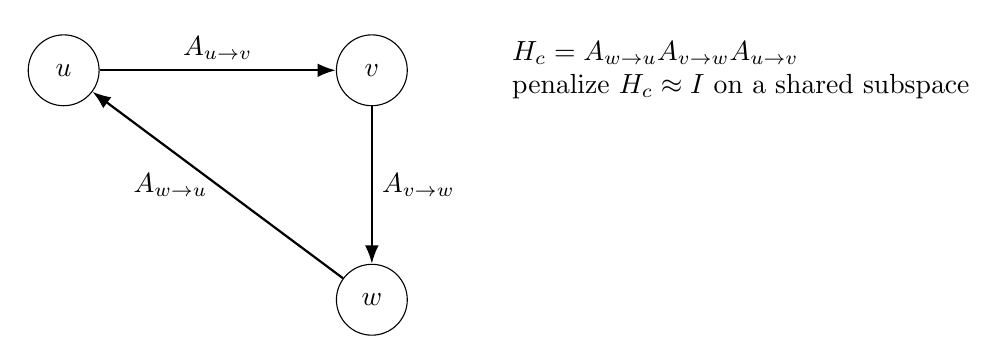
\begin{tikzpicture}[
  circ/.style={draw, circle, minimum size=0.9cm, align=center},
  edge/.style={-Latex, thick}
]
\node[circ] (u) {$u$};
\node[circ, right=3cm of u] (v) {$v$};
\node[circ, below=2cm of v] (w) {$w$};

\draw[edge] (u) -- node[above] {$A_{u\to v}$} (v);
\draw[edge] (v) -- node[right] {$A_{v\to w}$} (w);
\draw[edge] (w) -- node[left] {$A_{w\to u}$} (u);

\node[align=left, right=1.2cm of v] (txt) {$H_c=A_{w\to u}A_{v\to w}A_{u\to v}$\\
penalize $H_c\approx I$ on a shared subspace};
\end{tikzpicture}
\caption{Cycle composite (holonomy) as a consistency check for connectors around a directed cycle.}
\label{fig:holonomy}
\end{figure}

\subsection{Optimization schedule}
In practice, holonomy penalties are most effective when introduced in a staged manner:
\begin{enumerate}[leftmargin=2em]
\item initialize connectors from paired data or distillation (\cref{sec:connector-init});
\item apply norm/partial-isometry regularization on connectors to avoid ill-conditioning;
\item add holonomy penalties on a fundamental cycle basis;
\item only then unfreeze nonlinear modules participating in the cycle if task loss still requires it.
\end{enumerate}
This reduces the chance that the system ``uses'' gauge freedoms to hide inconsistency inside nonlinear modules.

\subsection{Elliptic complexes on quiver cycles: Hodge theory and a cyclic generalization}
\label{sec:elliptic}

Holonomy penalties provide a direct ``cycle error'' signal, but they do not by themselves explain \emph{how} inconsistency distributes across a larger cyclic subgraph, nor do they expose structured, low-dimensional summaries beyond per-cycle matrices.
A complementary viewpoint comes from \emph{elliptic complexes \`a la Atiyah~\cite{AtiyahSingerIndex}}: sequences of linear differential operators whose associated Laplacians are elliptic, yielding finite-dimensional cohomology spaces that capture \emph{global obstructions} to local solvability.
In our setting, the obstruction is precisely global cycle inconsistency.

We emphasize a \textbf{discrete, computable} specialization: a cycle basis turns a cyclic quiver into a finite cell complex, and linearized/connector-induced maps yield sparse operators whose spectra can be monitored during training.

\subsubsection{A discrete de Rham complex on a cycle basis}
Fix a cycle basis $\mc{C}$ (\\cref{alg:cycle-basis}) and attach one oriented 2-cell (``face'') for each $c\in\mc{C}$.
This yields a finite 2-complex with vertices $\Nodes$, edges $\Edges$, and faces $\mc{C}$.
To avoid any assumption of matched ambient dimensions, we work on a \emph{shared subspace} per port when needed (\\cref{sec:gauge}): choose orthonormal bases $U_v\in\R^{d_v\times r}$ and restrict connectors as
\[
A_e^{(r)} := U_{\tgt(e)}^\top A_e\, U_{\src(e)}\in\R^{r\times r}.
\]
All constructions below are differentiable in $A_e$ and (if learned) in $U_v$.

Define cochain spaces
\[
C^0 := \bigoplus_{v\in\Nodes} \R^{r},
\qquad
C^1 := \bigoplus_{e\in\Edges} \R^{r},
\qquad
C^2 := \bigoplus_{c\in\mc{C}} \R^{r},
\]
interpreted respectively as vertex potentials, edge residuals, and face curvatures \emph{expressed in a common $r$-dimensional frame}.
The covariant coboundary (discrete ``connection derivative'') $D_0:C^0\to C^1$ is
\[
(D_0 x)_e := x_{\tgt(e)} - A_e^{(r)} x_{\src(e)}.
\]
If $x_v$ represents an embedding in a shared coordinate system, then $(D_0 x)_e$ is the mismatch on edge $e$ after parallel transport by $A_e^{(r)}$.

A face operator $D_1:C^1\to C^2$ aggregates edge residuals around each basis cycle.
To sum in a common frame, we transport each residual to a chosen basepoint of the cycle.
Let $c=(e_1,\ldots,e_k)$ be an oriented cycle with base vertex $v_0=\src(e_1)$.
For each edge $e_j:u_j\to u_{j+1}$ on $c$, define the transport from $\tgt(e_j)=u_{j+1}$ back to $v_0$ as the restricted connector composite
\[
T_{c,e_j} := A_{e_1}^{(r)} A_{e_2}^{(r)}\cdots A_{e_{j}}^{(r)} \in \R^{r\times r}.
\]
Then define
\[
(D_1 \omega)_c := \sum_{j=1}^{k} T_{c,e_j}\,\omega_{e_j},
\qquad \omega\in C^1.
\]
If connectors are close to isometries (a training goal), $T_{c,e_j}$ is well-conditioned and this transport is numerically stable.
When using pseudo-inverse holonomy (\\cref{sec:gauge}), replace $T_{c,e_j}$ with a stabilized transport.

\paragraph{Curvature as failure of exactness.}
In a flat (globally consistent) configuration, $D_1 D_0 = 0$ and we obtain an honest complex
\[
C^0 \xrightarrow{D_0} C^1 \xrightarrow{D_1} C^2,
\qquad D_1D_0=0,
\]
a discrete analog of the de Rham elliptic complex.
In a general configuration, $D_1D_0$ measures \emph{curvature}: it is a structured version of the holonomy error.

\subsubsection{Hodge Laplacians and harmonic cycle modes}
Equip cochains with the standard Euclidean inner product (optionally weighted by edge/face confidences), inducing adjoints $D_0^\ast,D_1^\ast$.
The Hodge Laplacians are
\[
\Delta_0 := D_0^\ast D_0,\qquad
\Delta_1 := D_0 D_0^\ast + D_1^\ast D_1,\qquad
\Delta_2 := D_1 D_1^\ast.
\]
These are symmetric positive semidefinite and sparse/block-sparse.
In Atiyah's smooth setting, ellipticity guarantees good analytical properties; here the discrete analog is computational: $\Delta_k$ admits stable solvers and its small eigenvalues capture global structure.

\paragraph{Interpretation.}
Given an observed edge mismatch vector $\omega\in C^1$ (e.g., $\omega_e = U_{\tgt(e)}^\top y_{\tgt(e)} - A_e^{(r)} U_{\src(e)}^\top y_{\src(e)}$ on a batch),
a Hodge decomposition separates
\[
\omega = D_0 x \;+\; D_1^\ast \eta \;+\; h,
\]
where $D_0 x$ is an ``exact'' (vertex-potential) component, $D_1^\ast\eta$ is a ``coexact'' (face) component, and $h\in\ker(\Delta_1)$ is \emph{harmonic}.
The harmonic component corresponds to persistent global cycle modes not removable by local connector tweaks or face adjustments.
Monitoring $\|h\|^2$ and the smallest nonzero eigenvalues of $\Delta_1$ yields a principled diagnostic for ``where inconsistency lives''.

\begin{algorithm}[t]
\caption{Hodge diagnostics on a cycle basis (edge-space harmonic energy)}
\label{alg:hodge}
\begin{algorithmic}[1]
\Require restricted connectors $\{A_e^{(r)}\}$, cycle basis $\mc{C}$, edge residuals $\omega\in C^1$
\State build sparse matvecs for $D_0,D_1$ and their adjoints (block-sparse with $r\times r$ blocks)
\State define edge Laplacian operator $\Delta_1(\cdot)=D_0D_0^\ast(\cdot)+D_1^\ast D_1(\cdot)$
\State compute a few smallest eigenpairs $(\lambda_i, q_i)$ of $\Delta_1$ via Lanczos/LOBPCG
\State harmonic projector $P_h \gets \sum_{i:\lambda_i\le \epsilon} q_i q_i^\top$ (choose $\epsilon$ small)
\State harmonic component $h \gets P_h\,\omega$ and energy $E_h\gets \|h\|^2$
\State \Return $(E_h,\{\lambda_i\},h)$
\end{algorithmic}
\end{algorithm}

\paragraph{Training use.}
Computing eigenpairs every step is unnecessary.
In practice, use \cref{alg:hodge} intermittently as a diagnostic; during training use cheaper surrogates such as $\|D_1\omega\|^2$ (cycle curvature energy) and $\|D_0^\ast\omega\|^2$ (vertex divergence energy).
These are both differentiable and require only sparse matvecs.

\subsubsection{Cyclic elliptic complexes (twisted de Rham on a directed cycle)}
For a single directed cycle $c=(v_0\to v_1\to\cdots\to v_{k-1}\to v_0)$ with restricted connectors $A_i^{(r)}$, the operator $D_0$ reduces to a \emph{periodic covariant difference}
\[
(D_c x)_i = x_{i+1} - A_i^{(r)} x_i,\qquad i\in\bb{Z}/k\bb{Z},
\]
a discrete analog of the de Rham differential on $S^1$ with coefficients in a (learned) vector bundle.
The associated Laplacian $\Delta_c=D_c^\ast D_c$ is a \emph{cyclic elliptic operator}: it is block-circulant when $A_i^{(r)}$ is constant along the cycle and block-sparse in general.
Its small eigenvalues correspond to \emph{almost-parallel} sections---near-invariants transported around the loop.
Concretely, if the cycle holonomy $H_c=\prod_i A_i^{(r)}$ has eigenvalues close to $1$, then $\Delta_c$ has near-zero modes.
Thus holonomy control (\cref{sec:gauge}) and cyclic-elliptic spectra provide consistent, mutually reinforcing diagnostics.

\paragraph{Cyclic elliptic complexes and cyclic cohomology invariants.}
At the operator-algebra level, directed cycles correspond to elements of the quiver path algebra (\cref{sec:path-algebra,sec:operator-algebra}).
Cyclic functionals (traces) on these products define invariants that are stable under conjugation (gauge); in finite-dimensional realizations this reduces to computable quantities such as $\tr(H_c^m)$ or $\det(H_c)$.
This is a pragmatic shadow of cyclic cohomology~\cite{ConnesNCG}: we use it not for abstraction, but to motivate trace-based penalties and features that depend only on the cycle class, not on a particular traversal.



\newpage

\section{Computable invariants and diagnostics}
\label{sec:invariants}

A recurring pain point in modular ML is that failures are difficult to localize: is the issue an interface mismatch, an unstable loop, a router collapse, or a data deficiency?
We therefore advocate for a small set of \emph{computable invariants and diagnostics} that can be evaluated on a running system with modest overhead.

\subsection{A toolbox of invariants}
\Cref{tab:invariants} summarizes diagnostics that are (i) implementable, (ii) interpretable, and (iii) useful for training-time regularization.

\begin{table}[t]
\centering
\small
\begin{tabular}{p{3.3cm}p{6.1cm}p{3.9cm}}
\toprule
\textbf{Quantity} & \textbf{Definition / estimator} & \textbf{Use / interpretation} \\
\midrule
Connector norm &
$\opnorm{A_e}$ via power iteration; or $\Frob{A_e}$ &
Caps amplification; predicts exploding activations/gradients \\
\addlinespace
Partial isometry defect &
$\Frob{A_e^\top A_e-I}^2$ (tall) or $\Frob{A_e A_e^\top-I}^2$ (wide) &
Stabilizes interfaces under dimension mismatch; preserves geometry \\
\addlinespace
Cycle holonomy / curvature &
$H_c=\prod_{e\in c} A_e$, penalty $\Frob{H_c-I}^2$ or $\Frob{\log(H_c)}^2$ (restricted) &
Detects global embedding inconsistency in cycles; stabilizes feedback \\
\addlinespace
Local Jacobian spectral radius &
$\rho(D\Phi(z))$ estimated by power iteration on Jacobian-vector products &
Predicts contraction vs. instability for fixed-point execution \\
\addlinespace
	Tropical growth / cycle mean &
	Activation-fan fit plus max-plus cocycle growth $\chi_{\mathrm{trop}}$ or maximum cycle mean from \cref{alg:tropical-cocycle} &
	Global cycle stability/mixing; identifies expanding cells, slow modes, and recurrent bottlenecks \\
\addlinespace
Commutator norms &
$\norm{T_iT_j-T_jT_i}$ on linearized operators / connectors &
Checks symmetry transfer and order-insensitivity assumptions \\
\addlinespace
Hodge Laplacian spectrum (cycle space) &
Smallest eigenvalues of $\Delta_1 = D_0 D_0^\ast + D_1^\ast D_1$ on a cycle basis (\cref{sec:elliptic}); estimate via Lanczos/LOBPCG &
Localizes persistent global inconsistency; quantifies ``harmonic'' cycle modes not removable by local connector tweaks \\
\addlinespace
	Ergodic mixing / effective sample size &
	Integrated autocorrelation time $\widehat{\tau}_{\mathrm{int}}$ of key observables (\cref{alg:ergodic}) &
	Detects slow mixing or attractor collapse; sizes trajectory windows for tropical fan and cocycle estimates \\
\addlinespace
Reasoning-flow enstrophy (vorticity proxy) &
$\|\Omega(z)\|_F^2$ with $\Omega=\tfrac12(\nabla u-\nabla u^\top)$ for a learned velocity field $u$ (\cref{sec:fluid}) &
Penalizes turbulent vortices / circular reasoning; encourages stable, resource-efficient trajectories \\
\addlinespace
Path contribution / routing entropy &
$\pi_p(x)$ entropy; or variance of path outputs &
Detects router collapse; encourages diversity \\
\bottomrule
\end{tabular}
\caption{Computable invariants/diagnostics for decorated quivers.}
\label{tab:invariants}
\end{table}

\subsection{Learnable invariants}
\label{sec:learnable-invariants}

Some invariants are not known a priori but can be \emph{discovered} and exploited.

	\paragraph{Tropical invariants.}
	As in \cref{sec:tropical-cycle-dynamics}, train a tropical rational observable $\varphi_\eta=g_\eta-h_\eta$ such that $\varphi_\eta(\Psi(z))\approx \varphi_\eta(z)$.
	These invariants can be used as:
\begin{itemize}[leftmargin=2em]
\item a \textbf{constraint}: enforce approximate conservation (useful in physics-informed or algorithmic cycles),
\item a \textbf{regularizer}: discourage spurious drift in cycles,
\item a \textbf{representation}: invariant features often transfer across graph rewrites and distillation.
\end{itemize}

\paragraph{Hodge--harmonic invariants from elliptic complexes.}
As developed in \cref{sec:elliptic}, attaching a cycle basis and forming a discrete elliptic complex yields an edge-space Hodge Laplacian $\Delta_1$ whose near-kernel captures \emph{global} cycle modes.
Projecting edge residuals (or connector log-holonomies) onto a small set of harmonic eigenvectors produces low-dimensional, gauge-robust features.
These can be used as:
(i) diagnostics (which cycle modes persist despite connector tuning),
(ii) regularizers (penalize harmonic energy), or
(iii) \emph{learnable invariants} when the task admits true cyclic conservation laws.

\paragraph{Ergodic averages as invariants.}
For an ergodic cycle (\cref{sec:ergodic}), the time average of any integrable observable is an invariant of the long-run behavior.
Practically, we can \emph{learn} an observable $f_\eta$ and use its running average
$\bar f_T=\frac1T\sum_{t<T} f_\eta(z_t)$
as a stable summary feature for downstream prediction or as an auxiliary constraint.
This is a differentiable alternative to discrete memory retrieval: the ``memory'' is stored in the evolving continuous state and in learned invariant summaries of its trajectory.

\paragraph{Flow invariants in embedding-native reasoning.}
In embedding-fluid formulations (\cref{sec:fluid}), classical quantities such as circulation and enstrophy motivate computable penalties.
While the analogy is imperfect in high dimension, the \emph{antisymmetric Jacobian energy} $\|\Omega\|_F^2$ is a practical proxy for ``vorticity'' and correlates with circular, self-reinforcing updates.
We treat these as learnable invariants/constraints on the \emph{trajectory generator} (controller) rather than on discrete token sequences.

\paragraph{Energy-like Lyapunov functions.}
In fixed-point semantics, stability can be enforced by learning an energy $V_\eta(z)\ge 0$ such that $V_\eta(\Psi(z))\le V_\eta(z)$.
While constructing a true Lyapunov function is difficult in general, a soft penalty
\[
L_V = \E_z\left[\max(0, V_\eta(\Psi(z))-V_\eta(z)+\epsilon)\right]
\]
is implementable and often sufficient to discourage explosive cycles.

\paragraph{Symmetry-based invariants.}
If a group action $S_g$ is known (e.g., permutation invariance, rotation), invariants can be defined by averaging observables over the group or by enforcing commutation as in \cref{sec:operator-algebra}.
When composing pretrained modules with different internal bases, learned connectors can transfer symmetry approximately.

\subsection{Diagnostics as training-time instrumentation}
\label{sec:instrumentation}

We recommend treating the quiver as an instrumented program:
\begin{itemize}[leftmargin=2em]
\item log connector norms and partial-isometry defects per edge,
	\item periodically compute holonomy on a cycle basis,
	\item for each cyclic subgraph, estimate occupied activation fans, tropical growth rates, and boundary-hit rates on a small batch of trajectories,
	\item track routing entropy for routers/gating nodes.
\end{itemize}
These quantities are low-dimensional and can be plotted over time.
A typical failure mode is visible as a sudden spike in $\opnorm{A_e}$ or a drift in holonomy.

\subsection{Failure modes and how diagnostics disambiguate them}
\label{sec:diag-failures}

Diagnostics help separate qualitatively different issues:
\begin{itemize}[leftmargin=2em]
	\item \textbf{Interface mismatch in a cycle:} holonomy increases; tropical growth becomes positive or concentrated on a small subfan; connector norms often grow.
\item \textbf{Unstable fixed point solver:} Jacobian spectral radius estimate exceeds $1$; Anderson/Broyden iterations diverge.
\item \textbf{Router collapse:} routing entropy drops; path contribution variance concentrates on one path.
\item \textbf{Module underfitting:} task loss high but invariants remain stable; suggests adding capacity or data rather than re-wiring.
\end{itemize}

\newpage

\section{Learning the graph: continuous GFlowNet search over modular quivers}
\label{sec:gflownet}

A modular system design problem is naturally multiobjective: maximize task performance while respecting resource constraints (latency, VRAM, energy) and stability constraints (cycle contraction, holonomy).
Rather than optimize a single architecture, we often want \emph{a set} of high-performing graphs under different trade-offs.
GFlowNets provide an explicit mechanism for sampling diverse objects proportionally to a reward.

\subsection{Graph space}
Let $\mc{M}=\{N^{(k)}\}_{k=1}^K$ be a library of module templates (e.g., encoders, decoders, predictors, planners, routers), each with typed ports.
An admissible decorated quiver $g\in\mc{G}$ consists of:
\begin{itemize}[leftmargin=2em]
\item a directed multigraph structure $Q_g=(\Nodes_g,\Edges_g)$ with module choices $N_v\in\mc{M}$,
\item connector parameters $\{P_e\}$ (matrices/tensors),
\item optional hyperparameters (unroll depths, solver choice, routing rules).
\end{itemize}

We assume hard constraints on admissibility, e.g.:
typed port compatibility, maximum number of modules, maximum cycle length, explicit source/sink boundary vertices, or enforced presence of required inputs/outputs.

\subsection{Reward design: accuracy, resources, and stability}
\label{sec:reward}

There are two coupled reward objects.
The first is a \emph{graph-level} reward used to sample diverse high-value quivers.
The second is a \emph{trajectory-level} reward used for continuous Graph-of-Thought or other embedding-space reasoning inside a fixed quiver.

\paragraph{Graph-level reward.}
Let $R_{\mathrm{graph}}(g)\ge 0$ be an unnormalized reward for a terminal graph $g$.
A practical choice is:
\[
\log R_{\mathrm{graph}}(g) =
\underbrace{\alpha\, \mathrm{Score}(g)}_{\text{task metric}}
-\underbrace{\beta\,\mathrm{Cost}(g)}_{\text{compute/energy}}
-\underbrace{\gamma\,\mathrm{Instab}(g)}_{\text{stability penalties}}
-\underbrace{\delta\,\mathrm{Size}(g)}_{\text{parameters/VRAM}},
\]
where:
\begin{itemize}[leftmargin=2em]
\item $\mathrm{Score}(g)$ is validation accuracy, log-likelihood, reward, or other task metric,
\item $\mathrm{Cost}(g)$ estimates latency/FLOPs/Joules (see \cref{app:resources}),
\item $\mathrm{Instab}(g)$ aggregates holonomy, Jacobian spectral radius, tropical growth penalties, and activation-boundary congestion for cyclic subgraphs,
\item $\mathrm{Size}(g)$ accounts for parameter count and activation memory.
\end{itemize}
Weights $(\alpha,\beta,\gamma,\delta)$ define trade-offs.
Alternatively, use a Pareto-front GFlowNet construction to sample non-dominated architectures without scalarization.

\paragraph{Trajectory-level reward for embedding-space reasoning.}
Fix a graph $g$ and let
\[
\tau=(z_0,a_0,z_1,a_1,\dots,z_T)
\]
be a continuous reasoning trajectory in its internal embedding space.
Let $\mathrm{Qual}(\tau)$ denote a task-quality score (reward-model value, verifier score, accuracy surrogate, scientific utility, or oracle feedback), let $\mathrm{Res}(\tau)$ denote resource use (time, memory, number of steps, expensive module calls), and let $\mathrm{Stab}(\tau)$ denote instability penalties (vorticity, boundary congestion, excessive tropical growth, or cyclic inconsistency).
When explicit behavioral steering is desired, $\mathrm{Stab}(\tau)$ may also include steering-corridor and occupancy penalties of the form introduced in \cref{sec:ergodic-steering}.
We define
\begin{equation}
\Reward_{\mathrm{traj}}(\tau\mid g)
=
\mathbbm{1}\{\mathrm{Res}(\tau)\le B\}\,
\exp\!\Bigl(
\eta_1 \,\mathrm{Qual}(\tau)
-\eta_2 \,\mathrm{Res}(\tau)
-\eta_3 \,\mathrm{Stab}(\tau)
\Bigr),
\label{eq:traj-reward}
\end{equation}
where $B$ is a hard resource budget.
The indicator enforces our first requirement directly:
trajectories are rewarded only when resource constraints are met.
The exponential term enforces the second:
among feasible trajectories, higher-quality solutions receive proportionally higher mass.

\begin{proposition}[GFlowNet proportionality for embedding trajectories]
If a continuous-action GFlowNet over trajectory space is trained to exact trajectory balance with terminal reward $\Reward_{\mathrm{traj}}(\tau\mid g)$, then its terminal trajectory distribution is proportional to \eqref{eq:traj-reward}.
\end{proposition}

\begin{proof}[Proof sketch]
This is the standard terminal-density statement for trajectory-balance GFlowNets: exact balance equates the total forward flow into a terminal object with its unnormalized reward. Applying the construction to continuous trajectory space yields terminal density proportional to $\Reward_{\mathrm{traj}}(\tau\mid g)$.
\end{proof}

\subsection{GFlowNet generation process over graphs}
A GFlowNet defines a stochastic policy over \emph{construction trajectories}.
A state $s_t$ is a partially constructed graph; an action $a_t$ modifies it.
Typical action types:
\begin{itemize}[leftmargin=2em]
\item add a vertex with module type and port types,
\item add an edge between existing vertices and choose which input port it targets,
\item propose continuous connector parameters for the new edge (or a distribution over them),
\item optionally add hyperparameters (solver type, unroll depth).
\end{itemize}

We emphasize \emph{hybrid actions}: discrete structure plus continuous connector parameters.
Continuous parameters can be produced by a density model (e.g., Gaussian over matrix factors) or by sampling low-dimensional parameterizations (low-rank factors, orthogonal matrices).

\subsection{Objective: trajectory balance}
Let $\tau=(s_0,a_0,\dots,s_T)$ be a construction trajectory ending at terminal object $x=g$.
Trajectory balance trains forward and backward policies such that, at optimum, terminal probabilities are proportional to the chosen reward.
Concretely, it enforces:
\[
\log Z + \sum_{t=0}^{T-1} \log P_F(a_t\mid s_t)
=
\log R_{\mathrm{graph}}(g) + \sum_{t=0}^{T-1} \log P_B(a_t\mid s_{t+1}),
\]
where $Z$ is a learned normalizer.
This avoids explicit summation over trajectories leading to the same terminal graph.
The same identity is reused later for internal reasoning trajectories by replacing $R_{\mathrm{graph}}(g)$ with $\Reward_{\mathrm{traj}}(\tau\mid g)$ or with a reward on terminal thought graphs obtained by marginalizing over trajectories.

\subsection{Continuous GFlowNets on embedding space as probability flows (``embedding fluid'')}
\label{sec:fluid}

Although this section focuses on \emph{graph} generation, the same continuous-action GFlowNet machinery can operate \emph{inside} a fixed graph to generate \emph{continuous reasoning trajectories} in embedding space (see the GoT memory loop in \cref{fig:got}).
This perspective is useful because it exposes additional, computable constraints that are \emph{native to continuous embeddings} and therefore compatible with backpropagation.

\subsubsection{From trajectory balance to a continuity equation}
Consider a continuous state space $Z\subseteq\R^{d}$ (or a product of typed spaces) and a controller that generates a trajectory by proposing continuous increments
\[
z_{t+1}=z_t+\Delta z_t,
\qquad
\Delta z_t\sim q_\phi(\,\cdot \mid z_t,t\,).
\]
A continuous GFlowNet assigns \emph{flow} to partial trajectories and enforces a conservation law: inflow equals outflow at intermediate states, while terminal states absorb flow proportional to reward.
In a small-step limit (view $t$ as a discretization of ``reasoning time''), the induced density $\rho_t(z)$ evolves according to a continuity equation
\[
\partial_t \rho_t(z) \;+\; \nabla\!\cdot\!\bigl(\rho_t(z)\,u_\phi(z,t)\bigr)
\;=\; \sigma_{\mathrm{src}}(z,t)\;-\;\sigma_{\mathrm{sink}}(z,t),
\]
where $u_\phi(z,t):=\E[\Delta z_t\mid z_t=z]/\Delta t$ is an effective velocity field and $\sigma_{\mathrm{src}},\sigma_{\mathrm{sink}}$ represent source/sink terms at boundary vertices and terminals (reward).
The probability current $J=\rho u$ is the \emph{embedding fluid}; sampled trajectories are Lagrangian pathlines.
The induced ``graph of thoughts'' is then a discretization of streamlines and visited regions of this fluid.
Within this viewpoint, the reward in \eqref{eq:traj-reward} is a boundary sink term:
high-quality feasible trajectories absorb more flow, so the terminal distribution concentrates proportionally on them.

\subsubsection{Navier--Stokes-inspired regularization of reasoning trajectories}
A common failure mode in cyclic reasoning loops is \emph{self-reinforcing rotation}: the state moves in circles, repeatedly reusing the same latent content without making progress (``circular reasoning'').
In the fluid view, such behavior corresponds to large \emph{vorticity} and poor dissipation.
This motivates adding differentiable constraints inspired by viscous fluid dynamics~\cite{TemamNS} and physics-informed/neural PDE relaxations~\cite{RaissiPINNs}.

Let $u_\phi:Z\to\R^{d}$ be a learned velocity field (implemented, e.g., as the mean step of $q_\phi$ or as a residual update network).
Define its Jacobian $J(z)=\nabla u_\phi(z)$ (available implicitly via autodiff).
A practical high-dimensional proxy for vorticity is the antisymmetric Jacobian part
\[
\Omega(z)\ :=\ \tfrac12\bigl(J(z)-J(z)^\top\bigr),
\qquad
\text{enstrophy proxy: }\ \|\Omega(z)\|_F^2.
\]
We combine three computable penalties:
\[
L_{\mathrm{NS}} \;=\;
\lambda_{\mathrm{vort}}\E\|\Omega(z_t)\|_F^2
\;+\;
\lambda_{\mathrm{div}}\E\bigl(\tr J(z_t) + \kappa\bigr)^2
\;+\;
\lambda_{\mathrm{smooth}}\E\|J(z_t)\|_F^2,
\]
where $\kappa\ge 0$ optionally enforces \emph{average contraction} (negative divergence) for stabilizing cycles, and expectations are over on-policy trajectory states.
All terms can be estimated without forming full Jacobians: $\|\Omega\|_F^2$ requires one JVP and one VJP per Hutchinson probe; $\tr J$ uses a single JVP (see \cref{app:fluid}).

\paragraph{Alignment with quiver-level objectives.}
The quiver-level reward already balances task quality and resource costs (\cref{sec:reward}).
$L_{\mathrm{NS}}$ aligns the \emph{trajectory generator} with the same global constraints:
low vorticity discourages unproductive cycles; contraction/smoothness reduces sensitivity and compute; and both complement holonomy and tropical activation-fan penalties on cyclic subgraphs (\cref{sec:gauge,sec:tropical-cycle-dynamics}).

\paragraph{Reward decomposition for continuous GoT.}
For continuous Graph-of-Thought reasoning we recommend the explicit decomposition
\[
\mathrm{Qual}(\tau)=
\lambda_{\mathrm{ans}}\,\mathrm{Ans}(\tau)
\lambda_{\mathrm{ver}}\,\mathrm{Verify}(\tau)
\lambda_{\mathrm{oracle}}\,\mathrm{Oracle}(\tau),
\]
\[
\mathrm{Res}(\tau)=
\lambda_{\mathrm{time}}\,T
\lambda_{\mathrm{mem}}\,\mathrm{Mem}(\tau)
\lambda_{\mathrm{tool}}\,\mathrm{ToolCalls}(\tau),
\]
with $\mathrm{Stab}(\tau)$ augmented by tropical-boundary hits and fluid penalties.
This makes the reward transparent:
feasible trajectories that solve the problem well receive exponentially more mass, but different high-quality trajectories are still sampled according to their reward rather than collapsed to a single greedy path.

\begin{algorithm}[t]
\caption{Fluid-regularized continuous GFlowNet fine-tuning for embedding-native reasoning loops}
\label{alg:fluid-gfn}
\begin{algorithmic}[1]
\Require differentiable loop dynamics $z_{t+1}=\Psi_\theta(z_t,a_t)$, controller $q_\phi(\Delta z_t,\ldots\mid z_t)$, reward $\Reward_{\mathrm{traj}}(\tau\mid g)$
\For{training iteration}
  \State sample trajectory $\tau=(z_0,a_0,\ldots,z_T)$ with $a_t\sim q_\phi(\cdot\mid z_t)$
  \State compute terminal reward $\Reward_{\mathrm{traj}}(\tau\mid g)$ from quality, resource, and stability terms
  \State compute GFlowNet loss (e.g., trajectory balance) using $\Reward_{\mathrm{traj}}(\tau\mid g)$
  \State compute $L_{\mathrm{NS}}$ from on-trajectory states $\{z_t\}$ using autodiff probes
  \State update $(\theta,\phi)$ by gradient descent on $L_{\mathrm{TB}} + L_{\mathrm{NS}}$
\EndFor
\end{algorithmic}
\end{algorithm}

The NS-inspired terms are not ``physics claims'' about actual fluids; they are implementable, geometry-aware regularizers on continuous trajectory generators.
They are particularly natural when the cyclic subgraph is already modeled as a neural ODE/continuous flow, but they remain applicable to discrete residual updates.

\subsection{Allowing cycles}
Graph generation should support cyclic architectures.
This affects both admissibility checks and reward evaluation:
\begin{itemize}[leftmargin=2em]
\item \textbf{Execution:} cyclic graphs require either unrolling or fixed-point solving during evaluation.
\item \textbf{Stability:} cycles need contraction or spectral regularization to prevent divergence.
\item \textbf{Search bias:} without stability penalties, the search may propose unstable cycles that look promising under short unrolls.
\end{itemize}
We therefore incorporate stability diagnostics (\cref{sec:cycles,sec:tropical-cycle-dynamics,sec:gauge}) into $R_{\mathrm{graph}}(g)$.

\subsection{Bi-level pipeline: search and training}
\label{sec:bilevel}

Evaluating $R_{\mathrm{graph}}(g)$ exactly is expensive because it requires training.
A pragmatic approach is bi-level:
\begin{enumerate}[leftmargin=2em]
\item \textbf{Inner loop:} given a sampled graph $g$, train only its connectors and a small subset of modules for a limited budget (few steps/epochs), using weight inheritance from previous evaluations.
\item \textbf{Outer loop:} update the GFlowNet policies using the observed reward $R_{\mathrm{graph}}(g)$ and trajectory balance.
\end{enumerate}

Key tricks for implementability:
\begin{itemize}[leftmargin=2em]
\item \textbf{Weight inheritance:} reuse module weights across graphs; only initialize new connectors/modules.
\item \textbf{Caching:} reuse module outputs for frozen modules on shared datasets.
\item \textbf{Off-policy replay:} store (graph, reward) pairs and train the GFlowNet from replay to reduce variance.
\end{itemize}

\begin{algorithm}[t]
\caption{Continuous GFlowNet search over decorated quivers (bi-level)}
\label{alg:gflownet}
\begin{algorithmic}[1]
\Require module library $\mc{M}$, dataset/oracle, resource budget $B$, GFlowNet params $\phi$
\State initialize forward/backward policies $P_F^\phi,P_B^\phi$ and normalizer $Z$
\State replay buffer $\mc{D}\gets\emptyset$
\For{outer iteration}
  \State sample trajectory $\tau\sim P_F^\phi$ to obtain terminal graph $g$
  \State warm-start weights for $g$ via inheritance; initialize new connectors
  \State \textbf{inner training:} train $g$ for budget $B$ (connectors + selected modules)
  \State estimate diagnostics (holonomy, tropical growth, boundary-hit rates, norms)
  \State compute reward $R_{\mathrm{graph}}(g)$
  \State store $(\tau,g,R_{\mathrm{graph}}(g))$ in $\mc{D}$
  \State update $\phi,Z$ by minimizing trajectory-balance loss on minibatches from $\mc{D}$
\EndFor
\end{algorithmic}
\end{algorithm}

\subsection{Continuous connector parameter proposals}
Proposing a full dense matrix as a continuous action is high-dimensional.
Practical approaches:
\begin{itemize}[leftmargin=2em]
\item sample low-rank factors $U,V$ (dimension $r(d_u+d_v)$),
\item sample orthogonal/partial-isometry matrices via Householder products or Cayley transforms,
\item sample from a small discrete set of connector templates (dense, low-rank, block) and then optimize continuous parameters by gradient descent in the inner loop.
\end{itemize}
The third option is often best: the GFlowNet proposes structure, while inner-loop training handles exact values.

\newpage

\section{Training modular quivers}
\label{sec:training}

Once a graph $g$ is selected (or sampled), we must train it reliably.
This is not identical to training a monolithic model because:
(i) modules may be pretrained and partially frozen,
(ii) connectors may require careful initialization and regularization,
(iii) cycles require stable execution (unrolling or fixed points),
(iv) supervision may arrive from multiple channels (data, synthetic rollouts, oracles).

\subsection{Three supervision channels}
\label{sec:supervision}

We distinguish three sources of supervision commonly present in modular systems.

\paragraph{(1) Dataset supervision.}
Standard labeled or self-supervised datasets provide direct losses on outputs.

\paragraph{(2) Oracle supervision.}
An external process provides expensive labels or rewards (simulation, experiment, human feedback).
This often defines the objective in scientific design or RL.

\paragraph{(3) Self-generated synthetic supervision.}
A graph can generate its own training signals by producing pseudo-labels, trajectories, or self-consistency constraints.
Examples: distillation from a teacher graph, cycle-consistency, or self-training from high-confidence predictions.

These three channels naturally align with modular graphs, which can expose intermediate representations to auxiliary losses.

\subsection{Staged training schedule}
A practical, stable schedule for a newly wired graph:
\begin{enumerate}[leftmargin=2em]
\item \textbf{Stage A (connectors only):} freeze nonlinear modules; train only connectors with dataset supervision and distillation losses.
\item \textbf{Stage B (cycle stabilization):} add holonomy and norm regularizers; monitor tropical/ergodic diagnostics for cyclic SCCs (\cref{sec:tropical-cycle-dynamics,sec:ergodic}); for embedding-native reasoning loops optionally add NS-inspired trajectory regularizers (\cref{sec:fluid}); stabilize fixed-point solvers if cycles exist.
\item \textbf{Stage C (selective unfreezing):} unfreeze a small subset of modules (typically near the output or those with strong mismatch) with a smaller learning rate.
\item \textbf{Stage D (distillation/compression):} optionally distill the graph into a smaller equivalent graph by enforcing relation constraints (\cref{sec:path-algebra}).
\end{enumerate}

\subsection{Distillation across graph boundaries}
\label{sec:distillation}

Let $g_T$ be a teacher graph and $g_S$ a student graph.
Distillation in modular systems is not only about final outputs; it can enforce \emph{interface contracts}:
match outputs of corresponding ports after connectors.
For a pair of graphs that share a subset of modules, we can distill intermediate embeddings:
\[
L_{\mathrm{distill}} = \sum_{v\in\mc{V}_\mathrm{shared}} \E_x \norm{y_v^{(S)}(x) - \tilde P_v(y_v^{(T)}(x))}^2,
\]
where $\tilde P_v$ is an optional connector aligning teacher and student embeddings.
This is especially useful when rewriting a graph while preserving behavior.

\subsection{Synthetic data and self-training}
When oracle labels are expensive, use the current graph to propose candidates, score them with the oracle, and retrain.
This resembles active learning and is naturally integrated with GFlowNet sampling.


\begin{algorithm}[t]
\caption{Training a decorated quiver with stability instrumentation}
\label{alg:train}
\begin{algorithmic}[1]
\Require graph $g$ with modules and connectors, loss components, cycle basis $\mc{C}$
\For{training step}
  \State sample minibatch of external inputs
  \State execute graph (DAG or cyclic solver) to obtain outputs and internal states
  \State compute task loss $L_{\mathrm{task}}$
  \State compute connector regularizers (norm, partial isometry)
  \State compute holonomy loss $L_{\mathrm{hol}}$ on $\mc{C}$
  \State optionally estimate tropical-invariance or cellwise-affine prediction loss on short trajectories
  \State total loss $L \gets L_{\mathrm{task}} + \lambda_{\mathrm{hol}} L_{\mathrm{hol}} + \lambda_{\mathrm{trop}} L_{\mathrm{trop}} + \cdots$
  \State update parameters by gradient descent
  \State log diagnostics: $\opnorm{A_e}$, $L_{\mathrm{hol}}$, routing entropy, solver residual
\EndFor
\end{algorithmic}
\end{algorithm}

\subsection{Handling cycles during training}
For unrolled cycles, standard backpropagation applies.
For fixed-point cycles, use implicit differentiation (see \cref{app:fixed-point}).
A pragmatic compromise is to train with short unrolls early (to allow gradients) and switch to implicit solving once contraction is established.

\newpage

\section{Architecture templates and case studies}
\label{sec:case-studies}

We now illustrate how diverse deep learning systems map to decorated quivers.
The emphasis is on \emph{composability}: each example decomposes into reusable modules with typed ports and learnable connectors.

\subsection{Diffusion / flow-matching as a narrow special case}
A diffusion sampler can be viewed as a cyclic graph in which a denoiser module $N_\theta$ is repeatedly applied with a time-conditioned connector.
The ``rollout'' structure (many repeated steps) is therefore a special case of cyclic execution with shared parameters.
In the quiver view, diffusion is useful primarily because it makes cycles explicit and motivates stability diagnostics.
However, modularity in practice is broader than repeated application of one module.

\subsection{Graph-of-thought (GoT) memory as a quiver}

A modern alternative to ``context stuffing'' with external artifacts is to treat memory and reasoning as a \emph{learned, persistent graph in embedding space} that is traversed and updated during inference.
The core design goal is \textbf{embedding-native reasoning}: once an external input has been encoded into an initial state embedding, all intermediate computation (memory access, thought expansion, subgoal refinement) remains in continuous spaces so that the entire loop is trainable by backpropagation.

\paragraph{Latent memory graph state.}
Let the memory state at step $t$ be a typed, weighted graph
\[
\mc{G}_t := (\mc{V}_M,\mc{E}_M,\; M_t,\; A_t,\; \tau),
\]
where:
(i) $\mc{V}_M=\{1,\dots,N\}$ is a fixed set of \emph{slots} (choose $N$ large enough for the task horizon);
(ii) $M_t\in\R^{N\times d_{\mathrm{mem}}}$ stores node embeddings (row $i$ is $m_{t,i}$);
(iii) $A_t\in[0,1]^{N\times N\times r}$ stores soft edge weights for $r$ relation types;
(iv) $\tau:\mc{V}_M\to\mc{T}$ assigns a type to each slot (optionally learned via a type embedding).
A binary ``exists'' mask can be represented continuously as $s_t\in[0,1]^N$ (slot occupancy), which allows differentiable creation/retirement of nodes by gating.

\paragraph{Embedding-native read and write.}
Let $z_t\in\Emb_{\text{state}}$ denote the current latent thought/state embedding (or a short latent sequence in $\R^{L_z\times d}$).
A differentiable read operator produces a context embedding $c_t\in\Emb_{\text{ctx}}$:
\[
q_t=W_q z_t,\quad
k_{t,i}=W_k m_{t,i},\quad
v_{t,i}=W_v m_{t,i},
\qquad
\alpha_{t,i}=\softmax_i\!\left(\frac{\ip{q_t}{k_{t,i}}}{\sqrt{d_k}} + b_{\mathrm{graph}}(A_t,i)\right),
\quad
c_t=\sum_i \alpha_{t,i} v_{t,i}.
\]
Here $b_{\mathrm{graph}}(A_t,i)$ is an optional \emph{graph bias} (e.g., a learned function of incoming/outgoing edge weights, a message-passing summary, or a Laplacian positional encoding); all choices remain differentiable.

A differentiable write operator updates $(M_t,A_t,s_t)$ using continuous action parameters.
One implementable template is a \emph{soft slot update}:
\[
u_t = W_u z_t,\qquad
w_t = \softmax(\,M_t W_w z_t\,)\in\Delta^{N-1},
\qquad
M_{t+1}=M_t + \eta\, w_t u_t^\top,
\]
with a similar residual update for edge weights (e.g., predicting rank-one updates to $A_t$ or updating only a sparse set of relation channels).
Soft selection $w_t$ replaces non-differentiable ``pick-a-node'' operations.
In practice, multihead variants (multiple $u_t$ and $w_t$) and gated updates (learn $\eta\in[0,1]$) improve stability.

\paragraph{Reasoning dynamics as a cyclic quiver.}
A minimal embedding-native GoT loop is:
\[
z_t \xrightarrow{\;\pi_\phi\;} (w_t,u_t,\Delta A_t) \xrightarrow{\;\mathrm{READ}\;} c_t \xrightarrow{\;N_g\;} z_{t+1} \xrightarrow{\;\mathrm{WRITE}\;} (M_{t+1},A_{t+1},s_{t+1}),
\]
where $N_g:\Emb_{\text{state}}\oplus\Emb_{\text{ctx}}\to\Emb_{\text{state}}$ is a learned ``reasoner'' update (e.g., a transformer block operating on latent tokens, an MLP with residual connections, or a small recurrent operator).
All arrows are differentiable maps between embedding spaces.
Crucially, conversion to discrete token sequences is \emph{not} part of the internal loop: it appears only at designated \emph{boundary} vertices that interface with the outside world (initial encoding at a root; final decoding at a sink).

\begin{figure}[t]
\centering
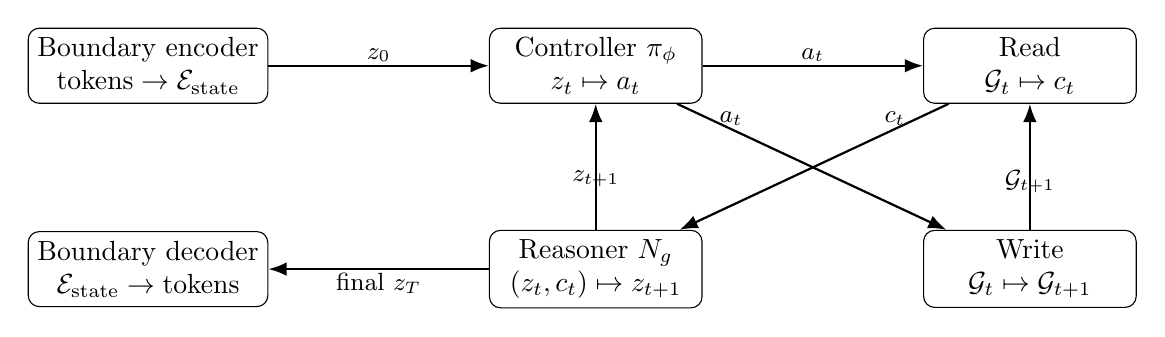
\begin{tikzpicture}[
  node/.style={draw, rounded corners, minimum width=2.7cm, minimum height=0.9cm, align=center},
  edge/.style={-Latex, thick},
  lab/.style={font=\small, inner sep=1pt}
]
\node[node] (Enc) {Boundary encoder\\$\text{tokens}\to \Emb_{\text{state}}$};
\node[node, right=2.8cm of Enc] (Ctl) {Controller $\pi_\phi$\\$z_t\mapsto a_t$};
\node[node, right=2.8cm of Ctl] (Read) {Read\\$\mc{G}_t\mapsto c_t$};
\node[node, below=1.6cm of Read] (Write) {Write\\$\mc{G}_t\mapsto \mc{G}_{t+1}$};
\node[node, below=1.6cm of Ctl] (Reason) {Reasoner $N_g$\\$(z_t,c_t)\mapsto z_{t+1}$};
\node[node, left=2.8cm of Reason] (Dec) {Boundary decoder\\$\Emb_{\text{state}}\to \text{tokens}$};

\draw[edge] (Enc) -- node[lab, above] {$z_0$} (Ctl);
\draw[edge] (Ctl) -- node[lab, above] {$a_t$} (Read);
\draw[edge] (Read) -- node[lab, above, pos=0.2] {$c_t$} (Reason);
\draw[edge] (Reason) -- node[lab, below] {$z_{t+1}$} (Ctl);
\draw[edge] (Ctl) -- node[lab, above, pos=0.2] {$a_t$} (Write);
\draw[edge] (Write) -- node[lab, below] {$\mc{G}_{t+1}$} (Read);
\draw[edge] (Reason) -- node[lab, below] {final $z_T$} (Dec);

\end{tikzpicture}
\caption{Embedding-native GoT memory loop as a cyclic decorated quiver.
All internal vertices operate on continuous embeddings; discrete tokenization appears only at boundary vertices (root encoder, sink decoder).}
\label{fig:got}
\end{figure}

\paragraph{Continuous GFlowNets for composable thought graphs.}
The controller can be trained as a \emph{continuous GFlowNet} that generates trajectories of memory operations.
Let a trajectory be $\tau=(a_0,\dots,a_{T-1})$ where each $a_t$ contains continuous parameters (soft node weights, update vectors, edge-weight deltas) and optional discrete \emph{termination} at $T$.
The terminal object is the induced \emph{thought graph} (e.g., nodes visited/updated with weights, plus the final memory state), and the reward combines:
task success (supervised loss or preference signal),
resource costs (latency, memory size, token budget at the \emph{boundary}),
and stability penalties (connector norms, holonomy on any cycles formed by memory relations).
Training with trajectory balance/detailed balance yields diverse high-reward reasoning traces rather than a single greedy trace.

\begin{algorithm}[t]
\caption{Embedding-native GoT memory: differentiable inference and (optional) GFlowNet fine-tuning}
\label{alg:got}
\begin{algorithmic}[1]
\Require boundary encoder/decoder, reasoner $N_g$, controller $\pi_\phi$, memory state $(M_0,A_0,s_0)$, horizon $T$
\State $z_0 \gets \mathrm{ENC}(\text{input tokens})$ \Comment{root boundary}
\For{$t=0,1,\dots,T-1$}
  \State $a_t \sim \pi_\phi(\,\mathrm{stop},\, w_t,u_t,\Delta A_t \mid z_t, M_t,A_t,s_t\,)$ \Comment{continuous parameters}
  \State $c_t \gets \mathrm{READ}(z_t; M_t,A_t,s_t; a_t)$ \Comment{soft attention / message passing}
  \State $z_{t+1} \gets N_g(z_t, c_t)$ \Comment{latent reasoning update}
  \State $(M_{t+1},A_{t+1},s_{t+1}) \gets \mathrm{WRITE}(z_t; M_t,A_t,s_t; a_t)$
  \If{$\mathrm{stop}$} \textbf{break} \EndIf
\EndFor
\State $\hat y \gets \mathrm{DEC}(z_T)$ \Comment{sink boundary}
\State compute task/stability loss and (optionally) a GFlowNet objective on trajectories
\State update $\phi$ and differentiable module parameters by gradient descent
\end{algorithmic}
\end{algorithm}

This construction is fully compatible with the quiver formalism: the memory state is a \emph{stateful vertex}, reads/writes are vertices, and connectors map between module bases.
Tropical diagnostics apply to the closed-loop map on $(z_t,M_t,A_t)$, enabling monitoring of ``memory drift'', nearly absorbing subfans, and slow activation-itinerary modes in reasoning.
\paragraph{Reasoning trajectories as pathlines in an embedding fluid.}
Because the controller policy and read/write operators are differentiable, the induced distribution over latent states $\{z_t\}$ can be treated as a \emph{probability flow} in continuous space.
In the continuous-action setting, trajectory balance enforces a conservation law on probability mass, which admits a natural ``fluid'' interpretation (\cref{sec:fluid}): $\rho_t(z)$ evolves under an effective velocity field $u_\phi(z,t)$ and trajectories are pathlines of the resulting probability current.
The \emph{embedding memory graph} is therefore a concrete discretization of visited regions and streamlines of this embedding fluid: nodes correspond to persistent regions/slots, and edges encode differentiable transport between them.

\paragraph{Navier--Stokes-style constraints against circular reasoning.}
If the loop repeatedly revisits the same latent states without improving task-relevant outputs, we observe (empirically) two signatures:
(i) high rotational components in the state update (``vortices''), and
(ii) slow mixing/large autocorrelation times (\cref{sec:ergodic}).
Both can be addressed without leaving embedding space by adding NS-inspired regularizers on the controller's velocity field (\cref{sec:fluid}):
penalize an enstrophy proxy $\|\Omega\|_F^2$ to reduce turbulent vortices, enforce mild contraction via divergence control to stabilize cycles, and penalize Jacobian energy to reduce sensitivity and compute.
These constraints complement holonomy penalties at the quiver level: holonomy targets \emph{representation inconsistency} around explicit graph cycles, while enstrophy targets \emph{trajectory-level} circularity inside a stateful vertex.

\paragraph{Multi-modal reasoning trajectories via smooth arrows.}
In many systems the loop state is multi-modal (text/vision/action), represented as a product embedding $z=(z^{(1)},\ldots,z^{(m)})$.
The same fluid/ergodic diagnostics apply on the concatenated state (or per-modality blocks), and connectors/arrows provide smooth changes of variables between modalities via learnable projections and joint-space fusion (\cref{sec:modal-smooth}).
Thus ``reasoning trajectories'' generalize beyond text: a cycle can traverse different modalities while remaining differentiable end-to-end, with any discrete tokenization confined to boundary vertices.

\subsection{Continuous GoT embedding-space reasoning with constrained rewards}
\label{sec:got-constrained}

The previous subsection described the mechanism.
Here we state the reward structure more formally.
Fix a source encoder $E:\Tok_{\mathrm{in}}\to \Emb_{\mathrm{state}}$ and sink decoder $D:\Emb_{\mathrm{state}}\to \Tok_{\mathrm{out}}$.
Let $g_{\mathrm{GoT}}$ denote the internal quiver of read, write, controller, and reasoner vertices.
An internal reasoning trajectory is
\[
\tau=(z_0,\mc{G}_0,a_0,z_1,\mc{G}_1,\ldots,z_T,\mc{G}_T).
\]
We define the terminal reward by
\[
\Reward_{\mathrm{GoT}}(\tau)
=
\mathbbm{1}\{\mathrm{Latency}(\tau)\le B_{\mathrm{time}},\ \mathrm{Mem}(\tau)\le B_{\mathrm{mem}}\}
\exp\!\Bigl(
\lambda_q\,Q(\tau)
-\lambda_t\,\mathrm{Latency}(\tau)
-\lambda_m\,\mathrm{Mem}(\tau)
-\lambda_s\,\mathrm{Stab}(\tau)
\Bigr),
\]
where $Q(\tau)$ measures solution quality after decoding $D(z_T)$ or after querying a verifier attached to the sink.
This is the precise constrained-reward statement requested by the research program:
resource-feasible trajectories receive probability mass proportional to a quality-weighted reward, while infeasible trajectories receive zero reward.

\paragraph{Tropical interpretation.}
The trajectory $\tau$ visits an empirical tropical atlas on the product space of latent thought states and memory graphs.
Reward-rich regions correspond to high-quality, low-cost, low-instability cells and cell transitions.
Architecture search and reasoning search are therefore aligned:
the outer GFlowNet looks for quivers whose internal tropical atlas admits many such high-reward trajectories, while the inner GFlowNet or controller concentrates flow on them.

\subsection{NatureLM and MDGen in a joint scientific embedding space}
\label{sec:naturelm-mdgen}

NatureLM provides a strong example of a \emph{source-heavy} scientific foundation model:
it operates on cross-domain scientific sequences and text, supporting text-to-science and science-to-science generation across molecules, proteins, materials, and nucleotides \cite{NatureLM2025}.
MDGen, by contrast, is a trajectory-generation model based on an SiT-style stochastic-interpolant or flow architecture over molecular-dynamics tokens \cite{MDGen2024}.
The quiver viewpoint suggests a principled way to combine them.

\paragraph{Boundary-aware factorization.}
Let
\[
E_{\mathrm{Nat}}:\Tok_{\mathrm{text/science}}\to \Emb_{\mathrm{nat}},
\qquad
E_{\mathrm{MD}}:\Tok_{\mathrm{traj\ seed}}\to \Emb_{\mathrm{md}},
\]
be source encoders for NatureLM-style inputs and MD seed states, and let
\[
D_{\mathrm{Nat}}:\Emb_{\mathrm{nat}}\to \Tok_{\mathrm{text/science}},
\qquad
D_{\mathrm{MD}}:\Emb_{\mathrm{md}}\to \Tok_{\mathrm{traj}}
\]
be sink decoders.
All interesting interaction happens internally:
adapters lift both embeddings into a joint space $\Emb_{\mathrm{joint}}$, a reasoning/controller cycle evolves there, and the resulting joint state steers the MDGen dynamics through typed projections and cross-attention arrows.

\paragraph{Why this is a natural tropical composition.}
NatureLM contributes a cross-domain semantic prior over scientific sequences and instructions.
MDGen contributes a structured trajectory prior over molecular motion.
The joint space then carries a composed tropical geometry:
NatureLM cells organize semantic or scientific constraints, MDGen cells organize trajectory-generation settings, and the adapters glue them into a common atlas on which a continuous reasoning trajectory can move.

\begin{figure}[t]
\centering
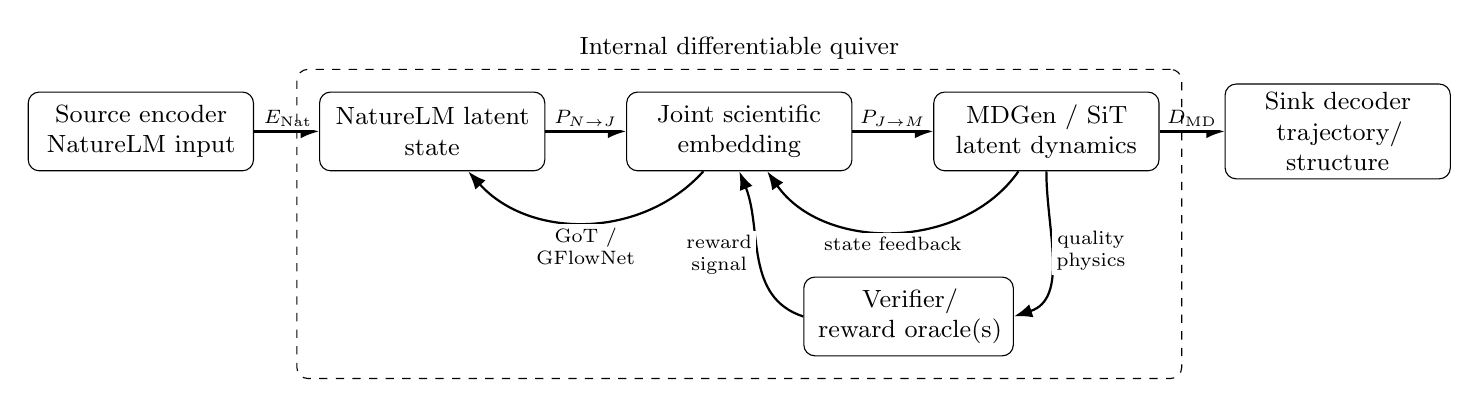
\begin{tikzpicture}[
  font=\small,
  node/.style={draw, rounded corners, text width=2.65cm, minimum height=1.0cm, align=center, inner sep=3pt},
  edge/.style={-Latex, thick},
  elab/.style={font=\scriptsize, align=center, fill=white, inner sep=1.5pt},
  box/.style={draw, dashed, rounded corners, inner sep=8pt}
]
\node[node] (natsrc) at (-2.3,1.0) {Source encoder\\NatureLM input};
\node[node] (nat) at (1.4,1.0) {NatureLM latent\\state};
\node[node] (joint) at (5.3,1.0) {Joint scientific\\embedding};
\node[node] (md) at (9.2,1.0) {MDGen / SiT\\latent dynamics};
\node[node] (sinktraj) at (12.9,1.0) {Sink decoder\\trajectory/ structure};
\node[node, text width=2.45cm] (ver) at (7.45,-1.35) {Verifier/ \\reward oracle(s)};

\draw[edge] (natsrc) -- node[elab, above, pos=0.52] {$E_{\mathrm{Nat}}$} (nat);
\draw[edge] (nat) -- node[elab, above, pos=0.5] {$P_{N\to J}$} (joint);
\draw[edge] (joint) -- node[elab, above, pos=0.5] {$P_{J\to M}$} (md);
\draw[edge] (md) -- node[elab, above, pos=0.5] {$D_{\mathrm{MD}}$} (sinktraj);
\draw[edge] (joint) to[out=228, in=312] node[elab, below, pos=0.5] {GoT /\\GFlowNet} (nat);
\draw[edge] (md.south) to[out=270, in=18] node[elab, right, pos=0.45] {quality\\physics} (ver.east);
\draw[edge] (ver.west) to[out=162, in=292] node[elab, left, pos=0.52] {reward\\signal} (joint.south);
\draw[edge] (md) to[out=235, in=305] node[elab, below, pos=0.5] {state feedback} (joint);

\node[box, fit=(nat)(joint)(md)(ver), label=above:{Internal differentiable quiver}] {};
\end{tikzpicture}
\caption{A quiver composition in which NatureLM-style scientific reasoning steers MDGen-style SiT molecular-dynamics generation through a joint embedding space. Source and sink vertices handle discrete sequences or trajectories; all steering and reward shaping occur in continuous embeddings.}
\label{fig:naturelm-mdgen}
\end{figure}

\paragraph{A concrete research workflow.}
NatureLM encodes a textual or sequence-based objective such as desired mechanism, binding context, or mutation constraint.
A controller in $\Emb_{\mathrm{joint}}$ proposes continuous reasoning displacements and adapter updates.
MDGen rolls out candidate dynamics conditioned on the joint embedding.
A verifier scores physical plausibility, target properties, and resource use.
The controller is then trained as a continuous GFlowNet whose trajectory distribution is proportional to a reward of the form \eqref{eq:traj-reward}.
This gives a mathematically coherent version of language-guided trajectory generation without forcing repeated decoding and re-encoding inside the loop.

\subsection{A realistic cycle of more than two models}
\label{sec:realistic-cycle}

Many application-rich programs need more than a pairwise composition.
The quiver formalism is particularly useful when the architecture is a genuine cycle with several model families and several feedback channels.
Consider the following stylized cycle:
\[
\substack{\text{generator} \to \text{ADFLIP evaluator} \to \text{structure oracle} \to \text{cell-state model} \\ \to \text{phenotype model} \to \text{controller} \to \text{generator}.}
\]
Each arrow is an adapter between typed embedding spaces.
Each vertex may be pretrained, partially frozen, or queried only occasionally.
The cycle is realistic because it mirrors multi-stage discovery pipelines in which proposals are repeatedly refined using progressively richer biological evidence.

\paragraph{Formal structure.}
Let
\[
z_t=
\bigl(
z_t^{\mathrm{gen}},
z_t^{\mathrm{ADFLIP}},
z_t^{\mathrm{struct}},
z_t^{\mathrm{cell}},
z_t^{\mathrm{variant}},
z_t^{\mathrm{morph}}
\bigr)
\]
be the product embedding state.
The cycle update is
\[
z_{t+1}=
\Psi(z_t)
=
\bigl(
\Psi_{\mathrm{gen}},
\Psi_{\mathrm{ADFLIP}},
\Psi_{\mathrm{struct}},
\Psi_{\mathrm{cell}},
\Psi_{\mathrm{variant}},
\Psi_{\mathrm{morph}}
\bigr)(z_t),
\]
where each component depends only on the ports receiving incoming arrows in the quiver.
The tropical atlas of the cycle then records which candidate classes, structural regimes, cell-state regimes, and phenotype regimes are occupied together.

\paragraph{Why a cycle rather than a chain.}
A chain can rank candidates once.
A cycle can refine them.
For instance, a poor ADFLIP prediction may be sent back to the generator through an adapter emphasizing the offending substructure; a morphology model may suggest a phenotypic failure mode that redirects attention toward a different region of sequence or conformational space; a cell-state model may expose compensatory pathways that require reconditioning the generator.
These are genuinely cyclic feedback mechanisms and belong in the theory, not outside it.

\subsection{Specific therapeutic-design instantiation}
\label{sec:therapeutic-cycle}

We now instantiate the previous pattern with the model families defined in the problem statement. The point is not to claim a finished benchmark, but to show that the research program yields a well-typed and implementable architecture.

\paragraph{Vertices.}
Use the following internal vertices:
\begin{itemize}[leftmargin=2em]
\item $N_{\mathrm{gen}}$: an RFdiffusion3-style or MDGen-style source generator for candidate structures or trajectories;
\item $N_{\mathrm{ADFLIP}}$: an ADFLIP-style inverse folding; 
\item $N_{\mathrm{struct}}$: a RosettaFold3- or Boltz-2-style structural oracle producing complex-structure or confidence embeddings;
\item $N_{\mathrm{cell}}$: a CellPLM-style cell-state response model producing transcriptomic or perturbational embeddings;
\item $N_{\mathrm{variant}}$: a VariantFormer-style regulatory or variant-effect predictor producing genotype-context embeddings;
\item $N_{\mathrm{morph}}$: a MorphoDiff-style phenotype or morphology generator or predictor producing image- or morphology-level embeddings;
\item $N_{\mathrm{ctl}}$: a continuous GFlowNet controller operating on the joint product space.
\end{itemize}

\paragraph{Edges and adapters.}
Each adjacent pair is linked by an adapter:
\[
P_{\mathrm{gen}\to \mathrm{adflip}},\ 
P_{\mathrm{adflip}\to \mathrm{struct}},\ 
P_{\mathrm{struct}\to \mathrm{cell}},\ 
P_{\mathrm{cell}\to \mathrm{variant}},\ 
P_{\mathrm{variant}\to \mathrm{morph}},\ 
P_{\mathrm{morph}\to \mathrm{ctl}},\ 
P_{\mathrm{ctl}\to \mathrm{gen}}.
\]
Additional shortcut edges may connect $N_{\mathrm{struct}}$ directly back to the controller or send cell-state summaries back to the generator.
All of these are admissible under the adapter semantics of \cref{sec:adapter-gluing}.

\begin{figure}[t]
\centering
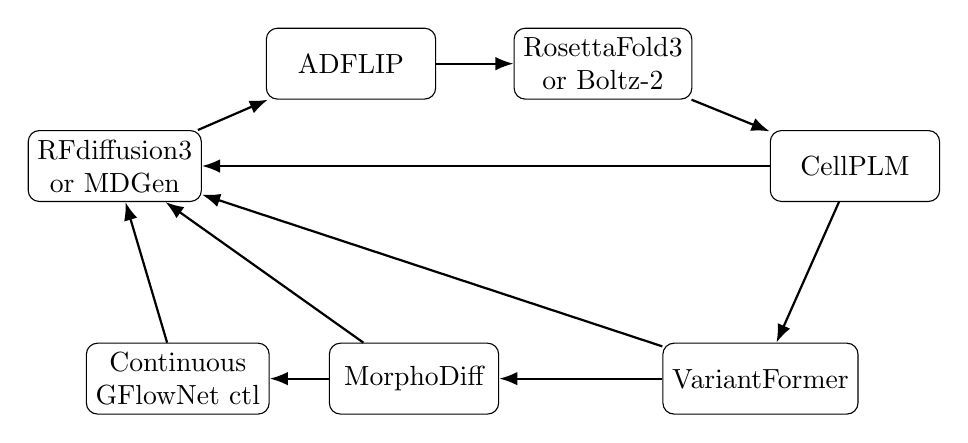
\begin{tikzpicture}[
  node/.style={draw, rounded corners, minimum width=2.15cm, minimum height=0.9cm, align=center},
  edge/.style={-Latex, thick}
]
\node[node] (gen) at (0,1.9) {RFdiffusion3\\or MDGen};
\node[node] (adflip) at (3.0,3.2) {ADFLIP};
\node[node] (struct) at (6.2,3.2) {RosettaFold3\\or Boltz-2};
\node[node] (cell) at (9.4,1.9) {CellPLM};
\node[node] (variant) at (8.2,-0.8) {VariantFormer};
\node[node] (morph) at (3.8,-0.8) {MorphoDiff};
\node[node] (ctl) at (0.8,-0.8) {Continuous\\GFlowNet ctl};

\draw[edge] (gen) -- (adflip);
\draw[edge] (adflip) -- (struct);
\draw[edge] (struct) -- (cell);
\draw[edge] (cell) -- (variant);
\draw[edge] (variant) -- (morph);
\draw[edge] (morph) -- (ctl);
\draw[edge] (ctl) -- (gen);
\draw[edge] (cell) to (gen);
\draw[edge] (variant) to (gen);
\draw[edge] (morph) to (gen);
\end{tikzpicture}
\caption{A six-model therapeutic-design cycle with a continuous GFlowNet controller. The quiver is realistic because each node plays a standard role in a discovery pipeline, while the cycle enables iterative refinement under tropical, ergodic, and resource-aware diagnostics.}
\label{fig:therapy-cycle}
\end{figure}

\paragraph{Reward and search objective.}
For a completed trajectory $\tau$ through this cycle, define
\[
\mathrm{Qual}(\tau)=
w_1\,\mathrm{Binding}(\tau)
+w_2\,\mathrm{ADFLIP}(\tau)
+w_3\,\mathrm{CellResponse}(\tau)
+w_4\,\mathrm{VariantRobustness}(\tau)
+w_5\,\mathrm{Morphology}(\tau),
\]
with each term normalized so higher is better.
Let $\mathrm{Res}(\tau)$ count wall-clock cost, expensive oracle calls, and memory.
Let $\mathrm{Stab}(\tau)$ aggregate tropical growth, holonomy defects, and fluid penalties.
Then \eqref{eq:traj-reward} defines a continuous GFlowNet target over therapeutic-design trajectories.
At the outer level, a graph GFlowNet mutates the quiver itself:
it may swap MDGen for RFdiffusion, replace RosettaFold3 by Boltz-2, insert extra adapters, or add shortcut edges.

\paragraph{Why TokenGT-style random-order decoding is natural here.}
Many outputs in this cycle are graph-like or structure-like:
residue interaction graphs, contact graphs, ligand graphs, and phenotype graphs.
A fixed left-to-right decoding order is therefore arbitrary.
The random-order TokenGT decoder from \cref{sec:random-order-decoding} is a natural sink mechanism:
it conditions on the currently revealed partial graph together with the full embedding-space context, and can decode important residues, uncertain motifs, or biologically constrained substructures first.
This matches the iterative refinement logic of the cycle better than a rigid serialization.

\paragraph{Why this example is mathematically useful.}
This cycle exercises nearly every part of the theory:
source and sink boundaries, heterogeneous embedding spaces, adapter gluing, tropicalized transformers, cyclic ergodic diagnostics, and hybrid continuous-discrete GFlowNet search.
It is therefore an ideal stress-test example for the manuscript.



\subsection{Mixture-of-experts (MoE) and routing graphs}
MoE layers are mixture-of-paths (\cref{sec:path-algebra}): a router selects among expert modules.
In a decorated quiver, the router is a vertex whose output is a distribution over outgoing edges, and each expert is a vertex.
Connector operators can be shared (parameter tying) or specialized.
Diagnostics include routing entropy and path contribution variance (\cref{sec:invariants}).

\subsection{World models with planning loops}
World-model agents typically consist of:
\begin{itemize}[leftmargin=2em]
\item encoder $N_e:\text{obs}\to \Emb_{\text{state}}$,
\item dynamics $N_f:\Emb_{\text{state}}\oplus \text{action}\to \Emb_{\text{state}}$,
\item reward model $N_r:\Emb_{\text{state}}\to \R$,
\item planner $N_p:\Emb_{\text{state}}\to \text{action sequence}$,
\item policy $N_\pi:\Emb_{\text{state}}\to \text{action}$.
\end{itemize}
Planning introduces cycles: planner proposes actions, dynamics predicts future states, and planner updates based on predicted outcomes.
Tropical diagnostics apply directly: the induced closed-loop dynamics has an activation fan and associated cocycle growth rates that reflect stability and exploration behavior.

\subsection{Neural operators + learned correctors}
In scientific ML, a common compositional pattern is:
\[
\text{coarse solver} \ \to\ \text{corrector}\ \to\ \text{physics-informed residual}.
\]
A neural operator predicts a coarse field; a refinement module (diffusion, flow matching, or deterministic residual network) adds corrections; a physics residual module enforces constraints or penalizes PDE residuals.
Connectors map between discretizations and channel layouts.
Holonomy penalties can enforce consistency when corrections are applied iteratively.

\subsection{Biological design with multi-fidelity endpoints}
Design pipelines often combine:
\begin{itemize}[leftmargin=2em]
\item a sequence model producing embeddings (PLM),
\item multiple property heads predicting biomarkers (stability, binding),
\item expensive oracles (wet-lab assays) providing endpoints,
\item a generative policy (GFlowNet) sampling candidates proportional to predicted utility and uncertainty.
\end{itemize}
This fits naturally: each predictor is a module; connectors are probes into embeddings; the GFlowNet is a graph-generation module that proposes new candidates; oracle feedback provides rewards.
Tropical invariants can appear when iterative refinement is used (e.g., repeated mutation proposals with acceptance criteria).

\subsection{Tool-use and agentic graphs}
Tool-using LLM systems naturally form quivers:
a controller module produces actions (tool calls), tool modules return observations, and a memory/state module aggregates.
Cycles are intrinsic: the agent loops until termination.
Stability is not contraction in Euclidean norm but \emph{policy stability} and \emph{distributional drift}; nonetheless, tropical diagnostics on learned state embeddings can quantify slow modes, nearly absorbing activation regions, and failure to converge.

\subsection{Graph-of-thought reasoning as a special case}

Graph-of-thought methods can be interpreted as explicit construction of a reasoning graph whose nodes are \emph{intermediate states} and whose edges are transformation operators.
For end-to-end differentiable training, the key constraint is that intermediate states should remain in continuous embedding spaces (latent ``thought tokens'' or state vectors), and edges should be differentiable maps (connectors, attention, message passing, residual updates).

If an implementation chooses to \emph{materialize} intermediate nodes as discrete token sequences (e.g., prompt $\to$ sampled text $\to$ prompt), then each such materialization is a boundary operation (decode $\to$ encode) that breaks gradient flow through the loop.
In the decorated-quiver view, these are explicit \emph{sink/root boundary vertices}; training must proceed by distillation across the boundary or policy-gradient style estimators.
The embedding-native GoT construction above avoids this pathology by keeping all intermediate computation inside the continuous quiver.

\newpage

\section{Implementation blueprint}
\label{sec:implementation}

This section outlines an implementation that is faithful to the theory and practical for modern deep learning stacks.
We assume PyTorch-like semantics, but the design transfers to JAX/Flax.

\subsection{Core data structures}
A minimal implementation needs:
\begin{itemize}[leftmargin=2em]
\item a \texttt{Node} object: module reference, port types, and parameter handle,
\item an \texttt{Edge} object: source node, target node, target port index, connector module,
\item a \texttt{Graph} object: adjacency lists; designated inputs/outputs; identification of cyclic subgraphs.
\end{itemize}

Typed ports can be represented as strings or enums; in code, they map to tensor shapes and packing/unpacking rules.

\subsection{Graph execution engine}
We recommend two execution backends:
\begin{itemize}[leftmargin=2em]
\item DAG executor using topological sort (fast, deterministic),
\item cyclic executor with either unrolling or fixed-point solving (Anderson/Broyden).
\end{itemize}
Cycles can be detected via strongly connected components (SCCs).
Each SCC is either acyclic (size 1 without self-loop) or cyclic.

\subsection{PyTorch skeleton for a decorated quiver module}
\begin{lstlisting}[language=Python,caption={Sketch of a decorated quiver executor with DAG evaluation. Cyclic SCCs are delegated to a solver.},label={lst:graph}]
import torch
import torch.nn as nn
from dataclasses import dataclass
from typing import Dict, List, Tuple, Any

@dataclass
class Edge:
    src: str
    tgt: str
    tgt_port: int
    connector: nn.Module  # maps src output -> tgt input port space

class QuiverGraph(nn.Module):
    def __init__(self, nodes: Dict[str, nn.Module], in_ports: Dict[str, int], edges: List[Edge]):
        super().__init__()
        self.nodes = nn.ModuleDict(nodes)
        self.in_ports = in_ports  # number of input ports per node
        self.edges = nn.ModuleList([e.connector for e in edges])
        self.edge_meta = edges    # keep metadata (src/tgt/port)

        # Build adjacency lists for fast execution
        self.in_edges: Dict[str, List[int]] = {k: [] for k in nodes.keys()}
        for idx, e in enumerate(edges):
            self.in_edges[e.tgt].append(idx)

    def forward(self, external_inputs: Dict[Tuple[str,int], torch.Tensor]) -> Dict[str, torch.Tensor]:
        # external_inputs maps (node_name, port_index) -> tensor
        topo = self._toposort_or_scc_order()
        outputs: Dict[str, torch.Tensor] = {}

        for v in topo:
            if self._is_cyclic_scc(v):
                outputs.update(self._solve_cyclic_scc(v, outputs, external_inputs))
                continue

            xs = [external_inputs.get((v,i), 0.0) for i in range(self.in_ports[v])]
            for ei in self.in_edges[v]:
                e = self.edge_meta[ei]
                src_out = outputs[e.src]
                msg = self.edges[ei](src_out)
                xs[e.tgt_port] = xs[e.tgt_port] + msg

            outputs[v] = self.nodes[v](*xs)
        return outputs

    # Implementations omitted: SCC decomposition, topo order within DAG,
    # fixed-point solver for cyclic SCCs, and caching for frozen modules.
\end{lstlisting}

\subsection{Handling cycles: solver choices and practical trade-offs}
\label{sec:cycle-impl}

For each cyclic SCC, choose one of:
\begin{itemize}[leftmargin=2em]
\item \textbf{Unrolling} for a fixed number of iterations $T$.
Pros: simple, standard autodiff. Cons: memory/time scale with $T$.
\item \textbf{Fixed-point solve} with Anderson or Broyden.
Pros: memory-efficient with implicit differentiation; robust when contraction holds.
Cons: requires stability diagnostics; solver may fail when dynamics is not contractive.
\end{itemize}
A robust training pipeline often uses unrolling early and transitions to fixed points after stabilization by connector regularizers and holonomy penalties.

\subsection{Resource estimation}
Architecture search and deployment require estimating cost.
We recommend:
\begin{itemize}[leftmargin=2em]
\item static parameter counts per module and connector,
\item analytical FLOPs for standard layers,
\item empirical latency models fit from profiling on target hardware.
\end{itemize}
\Cref{app:resources} gives formulas and a recommended measurement protocol.

\subsection{Tropical and holonomy instrumentation in code}
\label{sec:instrument-code}

Instrumentation can run on a small batch every $K$ steps.
Implementation tips:
\begin{itemize}[leftmargin=2em]
\item compute holonomy using stored connector matrices (no forward passes needed),
\item estimate connector norms via power iteration on $A_e$,
\item collect cycle trajectories by recording SCC states during execution,
\item run activation-fan estimation and cellwise affine fitting on CPU as background metrics (not in the training graph) or integrate a differentiable tropical-invariance loss for online regularization.
\end{itemize}

\newpage

\section{Limitations and failure modes}
\label{sec:limitations}

Our framework is intentionally pragmatic, but it has limitations.

\paragraph{Linear connectors may be insufficient.}
Some interfaces require nonlinear alignment (e.g., attention between modalities, normalization conditioned on context).
Our recommendation is to model such transforms as explicit module vertices.
Nevertheless, the ``edges are linear'' bias can restrict expressivity if misapplied.

\paragraph{Stability diagnostics are conservative.}
Contraction tests based on operator norms and Jacobian spectral radii can be pessimistic.
Tropical fan estimates depend on trajectory coverage and on how well the occupied cells have been explored.
In practice, use diagnostics as \emph{early-warning} signals rather than proofs.

\paragraph{Gauge non-identifiability complicates optimization.}
Even with holonomy and norm regularization, many equivalent parameterizations exist.
This can slow training or produce ill-conditioned connectors.
Practical mitigations include orthogonality constraints, per-node whitening, and staged training.

\paragraph{GFlowNet search cost.}
Graph search requires many evaluations.
Weight inheritance, caching, and proxy rewards are essential.
Even then, search is expensive for large libraries of modules and large graphs.
A practical approach is to restrict the search space via strong typing and small connector templates.

\paragraph{Non-differentiable boundary vertices.}
Some useful components---hard discrete search, symbolic solvers, and external tools---are not end-to-end differentiable.
They can still appear in a decorated quiver, but should be treated as explicit \emph{boundary} vertices (roots/sinks) where the system interfaces with the environment.
Internal reasoning and memory loops remain in embedding space and can be optimized by backprop; boundary interactions require distillation, surrogate losses, or policy-gradient style estimators.

\section{Discussion and open directions}
\label{sec:discussion}

We highlight directions that appear feasible in the near to mid term.

\paragraph{Tropical-guided cycle design.}
A promising angle is to treat activation-fan geometry and tropical growth targets as design constraints: enforce contraction for inference loops, mixing for sampling loops, and prescribed near-neutral subfans for memory.
This can be integrated into both training and architecture search.

\paragraph{Learnable invariants as transferable interfaces.}
Invariants discovered in one graph may persist under rewiring and distillation, providing a stable ``semantic basis'' for composition.
This suggests building module libraries that expose invariant-carrying ports explicitly.

\paragraph{Composable training recipes.}
Many modular systems are trained with ad hoc schedules.
A more systematic approach is to make instrumentation (holonomy, norms, tropical growth, activation occupancy, boundary-hit rates) part of the training loop and to trigger automatic interventions (freeze/unfreeze, learning-rate drops, connector re-initialization) based on diagnostics.

\paragraph{Graph compilation and deployment.}
Once graphs are expressed as decorated quivers with typed ports, they can be compiled: fuse linear connectors, prune unused paths, export to inference runtimes, and specialize to hardware constraints.
This is an engineering frontier where the quiver representation is directly useful.

\section{Conclusion}
\label{sec:conclusion}

We presented a unified framework for modular deep systems that models a system as a \emph{decorated quiver}: nonlinear modules at vertices connected by learnable (typically affine) connectors on edges.
This separation yields a practical calculus for composable architectures (path-algebra view), a set of operator-algebra and tropical-ergodic tools for analyzing and stabilizing cycles, and a toolbox of computable invariants (holonomy, tropical growth, Hodge energies, norms, and fluid diagnostics).
We also described an implementable pipeline for learning connectors and learning the graph itself via continuous GFlowNets under resource and stability constraints.
The goal is a pragmatic theory that attaches diagnostics and algorithms to the graphs practitioners already build.

\appendix

\section{Notation and minimal mathematical preliminaries}
\label{app:prelims}

This appendix records definitions used throughout, with an emphasis on implementable computation.

\subsection{Cycle space and fundamental cycles}
For a connected undirected graph with $|\Nodes|$ vertices and $|\Edges|$ edges, the dimension of the cycle space is $|\Edges|-|\Nodes|+1$.
A spanning tree $T$ has $|\Nodes|-1$ edges; each non-tree edge closes one fundamental cycle.
These cycles form a basis and can be found in $O(|\Nodes|+|\Edges|)$ time.

\subsection{Operator norms and power iteration}
For a matrix $A$, the operator norm $\opnorm{A}$ is the largest singular value.
Estimate it via power iteration on $A^\top A$ using matrix-vector products; this is differentiable if needed.

\section{Fixed-point solvers and implicit differentiation for cyclic SCCs}
\label{app:fixed-point}

This appendix provides implementable details for cyclic execution via fixed points.

\subsection{Anderson acceleration}
Given $z_{t+1}=\Phi(z_t)$, Anderson acceleration forms a linear combination of past residuals to accelerate convergence.
It is effective in deep equilibrium models and practical for cyclic quivers.

\subsection{Broyden's method}
Broyden approximates the inverse Jacobian of the residual $F(z)=z-\Phi(z)$.
It often converges faster but can be less stable; regularization is recommended.

\subsection{Implicit differentiation}
If $z^\star$ satisfies $F(z^\star,\theta)=0$, then
\[
\frac{\partial z^\star}{\partial \theta} = -\left(\frac{\partial F}{\partial z}\right)^{-1}\frac{\partial F}{\partial \theta},
\]
and gradients of a loss $L(z^\star)$ can be computed by solving a linear system with $(\partial F/\partial z)^\top$.
This is implementable with Jacobian-vector products.

\section{Tropical estimation recipes and code}
\label{app:tropical-estimation}

We expand on practical tropical estimation for modular cycles.

\subsection{Cellwise affine fitting in practice}
Choose a state representation $z_t$ for the cyclic SCC and log the activation-cell label $C_t$ during execution.
For every sufficiently occupied cell $C$, gather
\[
X_C=[z_t:\; C_t=C],\qquad Y_C=[z_{t+1}:\; C_t=C]
\]
and solve the ridge-regularized affine regression problem
\[
Y_C \approx A_C X_C + b_C \mathbf{1}^\top.
\]
This gives a cellwise affine model of the dynamics and is far more interpretable than a single global fit.

\subsection{A minimal activation-fan implementation}
\begin{lstlisting}[language=Python,caption={Cellwise affine fitting from logged activation labels.},label={lst:dmd}]
import torch

def fit_cellwise_affine(Z, Z_next, cell_ids, lam=1e-4, min_count=8):
    # Z, Z_next: (T, d), cell_ids: list/1D tensor of length T
    models = {}
    cells = torch.as_tensor(cell_ids)
    ones = torch.ones(Z.shape[0], 1, device=Z.device, dtype=Z.dtype)
    Z_aug = torch.cat([Z, ones], dim=1)  # affine lift
    for c in cells.unique():
        mask = cells == c
        if int(mask.sum()) < min_count:
            continue
        X = Z_aug[mask]                  # (n, d+1)
        Y = Z_next[mask]                 # (n, d)
        G = X.T @ X + lam * torch.eye(X.shape[1], device=Z.device)
        Theta = torch.linalg.solve(G, X.T @ Y)  # (d+1, d)
        A = Theta[:-1].T
        b = Theta[-1]
        models[int(c)] = {"A": A, "b": b}
    return models
\end{lstlisting}

\subsection{Using tropical growth as a regularizer}
A lightweight regularizer forms a max-plus weight matrix
\[
(M_C)_{ij}=\log(\varepsilon + |(A_C)_{ij}|),
\]
for occupied cells and penalizes positive tropical growth:
\[
L_{\mathrm{trop}}=\max(0,\widehat{\chi}_{\mathrm{trop}}-\tau).
\]
In practice one may estimate $\widehat{\chi}_{\mathrm{trop}}$ from long products along sampled itineraries, or from a maximum-cycle-mean computation on the occupied transition graph.

\section{Resource accounting}
\label{app:resources}

Resource-aware search and deployment require consistent units.

\subsection{FLOPs and latency}
Analytical FLOPs estimates can be derived for standard layers (matmul, conv).
Latency is hardware-dependent; we recommend fitting a calibration model from profiling runs and using it in rewards.

\subsection{VRAM and activation memory}
Activation memory depends on execution (unrolling vs. implicit).
Implicit differentiation can reduce memory by avoiding storage of all intermediate states.

\section{Additional architecture templates}
\label{app:templates}

We list additional composable templates not covered in \cref{sec:case-studies}.

\subsection{Energy-based sampling loops}
Combine a learned energy module $E_\theta$ with a sampler module (Langevin, HMC) in a cycle.
Tropical growth and transition entropy quantify mixing; holonomy checks connector consistency when energies are computed in multiple embedding spaces.

\subsection{Hybrid symbolic--neural pipelines}
A symbolic solver can be treated as an oracle module; connectors map neural embeddings to solver inputs and back.
Distillation can train a neural surrogate for the solver, enabling end-to-end training.

\section{Reproducibility checklist}
\label{app:repro}

For empirical work built on this framework:
\begin{itemize}[leftmargin=2em]
\item specify module library and port types,
\item report connector parameterizations and regularizers,
\item report cycle execution semantics (unroll depth or solver details),
\item log invariants: connector norms, holonomy, tropical growth, activation occupancy,
\item include ablations: with/without holonomy, with/without tropical regularization, connector rank.
\end{itemize}



\section{Stability analysis and contraction tests for cyclic quivers}
\label{sec:stability}

This appendix provides computable stability criteria for cyclic SCCs and practical methods to enforce them.
The goal is not to produce the sharpest possible bound; it is to provide \emph{tests and knobs} that work in code.

\subsection{Block norms on product spaces}
Let $Z=\prod_{v\in\Nodes_\mathrm{state}} Y_v$ be a product of (finite-dimensional) normed spaces.
A convenient family of norms is a weighted block-$\ell_\infty$ norm:
\[
\norm{z}_{\infty,w} := \max_{v\in\Nodes_\mathrm{state}} \frac{\norm{z_v}_2}{w_v},
\qquad w_v>0.
\]
This norm makes it easy to obtain sufficient contraction conditions by bounding each block update in terms of other blocks.

\subsection{A small-gain style sufficient condition}
Consider a cyclic SCC executed by the update map $z\mapsto \Phi(z)$.
Assume each module $N_v$ is (locally) Lipschitz in each input port:
\[
\norm{N_v(x)-N_v(x')}_2 \le \sum_{i=1}^{m_v} L_{v,i}\,\norm{x^{(i)}-x'^{(i)}}_2,
\]
where $x=(x^{(1)},\dots,x^{(m_v)})$.
Each connector $P_e(z)=A_e z+b_e$ is linear up to bias, and therefore Lipschitz with constant $\opnorm{A_e}$.

For a stateful vertex $v$, the update depends on messages from predecessors $u$ via edges $e:u\to v$.
Define an \emph{edge gain}:
\[
g_e := L_{v,i(e)}\,\opnorm{A_e}.
\]
Intuitively, $g_e$ upper bounds how much a perturbation in $y_u$ can affect $y_v$ through port $i(e)$.

Define a weighted adjacency operator on the state vertices:
\[
(G_w)_{v\leftarrow u} := \sum_{e:u\to v} g_e \frac{w_u}{w_v}.
\]
Then, under mild assumptions on aggregation (sum of messages), we obtain:
\begin{proposition}[Sufficient contraction condition]
If for some weights $w_v>0$,
\[
\max_{v}\ \sum_{u} (G_w)_{v\leftarrow u} \;<\; 1,
\]
then $\Phi$ is a contraction in the block norm $\norm{\cdot}_{\infty,w}$.
\end{proposition}

\paragraph{Choosing weights.}
A practical choice is to set $w$ to the Perron--Frobenius eigenvector of the unweighted gain matrix (or to all ones).
More robust: solve a linear program to minimize the maximum row sum of $G_w$ subject to $w_v\in[w_{\min},w_{\max}]$.

\subsection{Damped updates and contraction enforcement}
Even if the raw update is not contractive, a \emph{damped} update often is:
\[
z_{t+1} = (1-\eta)\,z_t + \eta\,\Phi(z_t),\qquad 0<\eta\le 1.
\]
If $\Phi$ is Lipschitz with constant $L$ (in some norm), then the damped map has constant $(1-\eta)+\eta L$.
Thus, if $L>1$ but not too large, choosing smaller $\eta$ can restore contraction.
In code, damping corresponds to residual connections at the SCC level and is easy to implement.

\subsection{Jacobian spectral radius estimation via JVPs}
Local stability at a fixed point is governed by the Jacobian $J=D\Phi(z^\star)$.
We rarely form $J$ explicitly.
Instead, estimate $\rho(J)$ or $\sigma_{\max}(J)$ using matrix-vector products, implemented as Jacobian-vector products (JVPs).

\begin{algorithm}[t]
\caption{Estimate $\sigma_{\max}(J)$ of a cyclic SCC update via power iteration}
\label{alg:power-jacobian}
\begin{algorithmic}[1]
\Require update map $\Phi$, state $z$ (treated as fixed), iterations $K$
\State sample random vector $v$ with $\norm{v}=1$
\For{$k=1$ to $K$}
  \State compute $u \gets J v$ via JVP at $z$: $u=\mathrm{JVP}(\Phi,z;v)$
  \State $v \gets u / \norm{u}$
\EndFor
\State \Return estimate $\sigma_{\max}(J)\approx \norm{u}$
\end{algorithmic}
\end{algorithm}

\begin{lstlisting}[language=Python,caption={PyTorch snippet for Jacobian-vector power iteration on an implicit SCC update.},label={lst:jvp}]
import torch
from torch.func import jvp  # PyTorch >= 2.0

def spectral_norm_estimate(phi, z, n_iter: int = 20):
    # z: tuple of tensors representing SCC state
    v = tuple(torch.randn_like(zi) for zi in z)
    # normalize v
    vnorm = torch.sqrt(sum((vi**2).sum() for vi in v))
    v = tuple(vi / (vnorm + 1e-12) for vi in v)

    for _ in range(n_iter):
        y, u = jvp(phi, (z,), (v,))  # u approximates J v
        unorm = torch.sqrt(sum((ui**2).sum() for ui in u))
        v = tuple(ui / (unorm + 1e-12) for ui in u)
    return unorm
\end{lstlisting}

\paragraph{When to trust this estimate.}
Power iteration estimates $\sigma_{\max}$, not $\rho$.
If the Jacobian is normal, $\sigma_{\max}=\rho$; otherwise $\sigma_{\max}$ upper bounds $\rho$.
Empirically, $\sigma_{\max}<1$ is a strong signal of stability.
If $\sigma_{\max}>1$, the SCC can still be stable, but divergence becomes more likely.

\subsection{Practical stability interventions}
When diagnostics indicate instability:
\begin{enumerate}[leftmargin=2em]
\item add damping at SCC level (reduce $\eta$),
\item tighten connector norm constraints (spectral normalization),
\item increase holonomy penalties for cycles (reduce inconsistent feedback),
\item reduce connector rank or enforce partial isometry,
\item freeze problematic nonlinear modules and retrain connectors,
\item switch from fixed-point execution to bounded unrolling with gradient clipping.
\end{enumerate}

\section{Holonomy computation details and optimization-friendly surrogates}
\label{app:holonomy}

This appendix expands \cref{sec:gauge} with implementation-level details.

\subsection{Cycle bases in directed graphs}
For holonomy penalties we need a set of cycles that span the cycle space of the underlying undirected graph.
In directed graphs, a directed cycle basis can be obtained by:
\begin{itemize}[leftmargin=2em]
\item compute SCCs; only SCCs with $\ge 2$ vertices (or a self-loop) can contain cycles,
\item within each SCC, ignore directions to build a spanning tree and fundamental cycles,
\item for each undirected fundamental cycle, choose an orientation consistent with the directed edges where possible; otherwise traverse edges in reverse by using pseudo-inverse connectors if needed.
\end{itemize}

\subsection{Holonomy losses under dimension mismatch}
We restate the two implementable approaches.

\paragraph{Shared-subspace restriction.}
Estimate a shared subspace basis $U\in\R^{d\times r}$ at the cycle entry.
Options:
\begin{itemize}[leftmargin=2em]
\item PCA on embeddings observed at the cycle entry,
\item CCA between entry embeddings and embeddings after one cycle pass,
\item learn $U$ as a Stiefel parameter (orthonormal columns) jointly with training.
\end{itemize}
Then compute $\tilde H_c=U^\top H_c U$ and penalize $\tilde H_c\approx I_r$.

\paragraph{Pseudo-inverse holonomy.}
Use Tikhonov pseudo-inverses $A^{\dagger_\lambda}$ and define a forward-backward consistency operator $\hat H_c$.
This checks that information sent around a cycle returns to the same subspace.

\subsection{Matrix logarithm vs. surrogates}
The matrix logarithm $\log(H)$ is well-behaved only when $H$ is close to $I$ and has no eigenvalues on the negative real axis.
In training, it is often sufficient to use:
\[
L_{\mathrm{hol}}^{\mathrm{sur}} = \Frob{H-I}^2
\quad \text{or} \quad
L_{\mathrm{hol}}^{\mathrm{svd}} = \sum_i (\sigma_i(H)-1)^2.
\]
The singular-value surrogate $L_{\mathrm{hol}}^{\mathrm{svd}}$ is stable even when $H$ is not diagonalizable and directly penalizes contraction/expansion around the cycle.

\subsection{Holonomy computation snippet}
\begin{lstlisting}[language=Python,caption={Compute holonomy on a cycle from connector matrices.},label={lst:holonomy}]
import torch

def cycle_holonomy(mats):
    # mats: list of matrices [A1, A2, ..., Ak] representing cycle order
    H = mats[0]
    for A in mats[1:]:
        H = A @ H
    return H  # square at cycle start dimension

def holonomy_surrogate_loss(H):
    d = H.shape[0]
    I = torch.eye(d, device=H.device, dtype=H.dtype)
    return torch.norm(H - I, p="fro")**2
\end{lstlisting}

\section{Elliptic-complex and Hodge diagnostics on quiver cycle space}
\label{app:elliptic}

This appendix provides implementable details for the discrete elliptic-complex/Hodge viewpoint introduced in \cref{sec:elliptic}.
The goal is not to ``do differential geometry'' in training loops; it is to obtain \emph{sparse linear-algebra operators} whose energies and spectra localize cycle inconsistency.

\subsection{Data structures}
Assume a (restricted) shared dimension $r$ and the following tensors:
\begin{itemize}[leftmargin=2em]
\item vertex count $n=|\Nodes|$, edge count $m=|\Edges|$;
\item integer arrays \texttt{src}, \texttt{tgt} of shape $(m,)$ giving endpoints;
\item restricted edge maps \texttt{A} of shape $(m,r,r)$ storing $A_e^{(r)}$;
\item optional cycle basis as a list of cycles, each cycle a list of edge indices (in traversal order).
\end{itemize}
The restriction bases $U_v$ are needed only to form $A_e^{(r)}$ and residuals; the Hodge operators operate in the common $r$-frame.

\subsection{Sparse matvecs for $D_0$ and $D_0^\ast$}
$D_0:C^0\to C^1$ acts on vertex potentials $x\in\R^{n\times r}$ and produces edge residuals $\omega\in\R^{m\times r}$:
\[
\omega_e = x_{\tgt(e)} - A_e^{(r)} x_{\src(e)}.
\]
Its adjoint $D_0^\ast:C^1\to C^0$ is
\[
(D_0^\ast \omega)_v
=
\sum_{e:\tgt(e)=v}\omega_e
\;-\;
\sum_{e:\src(e)=v} (A_e^{(r)})^\top \omega_e.
\]
Both can be implemented with gather + batched matmul + scatter-add.

\begin{lstlisting}[language=Python,caption={PyTorch matvecs for $D_0$ and $D_0^\ast$ (shared dimension $r$)},label={lst:d0}]
import torch

def D0(x, A, src, tgt):
    # x: (n,r), A: (m,r,r), src/tgt: (m,)
    x_src = x[src]                       # (m,r)
    x_tgt = x[tgt]                       # (m,r)
    Ax = torch.einsum("mij,mj->mi", A, x_src)
    return x_tgt - Ax                    # (m,r)

def D0_adj(omega, A, src, tgt, n):
    # omega: (m,r) -> out: (n,r)
    out = omega.new_zeros((n, omega.shape[1]))
    out.index_add_(0, tgt, omega)        # sum into targets
    A_T_omega = torch.einsum("mji,mj->mi", A, omega)  # A^T omega
    out.index_add_(0, src, -A_T_omega)   # subtract into sources
    return out
\end{lstlisting}

\subsection{Cycle operator $D_1$ and transport}
For each basis cycle $c=(e_1,\ldots,e_k)$ choose a basepoint (e.g., $\src(e_1)$).
Precompute transport matrices $T_{c,e_j}$ as prefix products of restricted connectors.
In code, store a list of per-cycle tensors \texttt{T\_cyc} with shape $(k,r,r)$ aligned with the cycle's edge list.

\begin{lstlisting}[language=Python,caption={Cycle aggregation $D_1$ and its adjoint $D_1^\ast$ with precomputed transports},label={lst:d1}]
def D1(omega, cycles, transports):
    # omega: (m,r)
    # cycles: list[list[int]] edge indices per cycle
    # transports: list[Tensor] each (k,r,r) for the corresponding cycle
    r = omega.shape[1]
    out = omega.new_zeros((len(cycles), r))
    for i, (cyc, T) in enumerate(zip(cycles, transports)):
        # gather omega on edges in this cycle: (k,r)
        om = omega[torch.tensor(cyc, device=omega.device)]
        # transport and sum: sum_j T_j @ om_j
        out[i] = torch.einsum("kij,kj->i", T, om)
    return out

def D1_adj(eta, cycles, transports, m):
    # eta: (|C|,r) -> omega_like: (m,r)
    out = eta.new_zeros((m, eta.shape[1]))
    for i, (cyc, T) in enumerate(zip(cycles, transports)):
        # distribute: omega_e += T_e^T @ eta_c
        contrib = torch.einsum("kji,j->ki", T, eta[i])  # (k,r)
        out.index_add_(0, torch.tensor(cyc, device=eta.device), contrib)
    return out
\end{lstlisting}

\paragraph{Note.}
If transports are expensive or connectors are already close to partial isometries, you can approximate $T_{c,e_j}\approx I$.
This yields a purely combinatorial $D_1$ (cycle-edge incidence) that is often sufficient as a diagnostic.
Transport-aware $D_1$ is more faithful when cycles include strong basis changes.

\subsection{Cheap Hodge energies and intermittent spectra}
The full harmonic projection in \cref{alg:hodge} requires eigenpairs of $\Delta_1$.
In most training loops it suffices to log the two energies
\[
E_{\mathrm{curv}}=\|D_1\omega\|^2,\qquad
E_{\mathrm{div}}=\|D_0^\ast\omega\|^2,
\]
which are cheap and differentiable.

When an eigen-spectrum is desired (e.g., once per epoch), form a \texttt{scipy.sparse.linalg.LinearOperator} that applies
$\Delta_1(\omega)=D_0D_0^\ast(\omega)+D_1^\ast D_1(\omega)$
via the matvecs above and call \texttt{eigsh} for the smallest eigenvalues.
This yields the ``harmonic mode'' diagnostics without materializing dense matrices.

\section{Operator-algebra regularizers in practice}
\label{app:opreg}

This appendix collects regularizers and diagnostics motivated by the operator-algebra viewpoint (\cref{sec:operator-algebra}) and emphasizes implementability.

\subsection{Commutator penalties and approximate symmetries}
Given operators $T_i,T_j$ (connectors, Jacobians, or cellwise affine/tropical approximants), the commutator
$[T_i,T_j]=T_iT_j-T_jT_i$ measures order sensitivity.
In modular systems, order sensitivity is often undesirable when two operations represent independent ``coordinate changes''.
A generic penalty:
\[
L_{\mathrm{comm}}(i,j) = \Frob{T_iT_j-T_jT_i}^2.
\]
In high dimensions, form $T_iT_j$ explicitly only if cheap; otherwise use randomized trace estimators:
\[
\Frob{C}^2 = \E_{\epsilon\sim\mc{N}(0,I)} \norm{C\epsilon}_2^2,
\]
estimated by a few random vectors.

\subsection{Intertwiner losses}
Suppose two modules implement related transformations under a known linear action $S$ (e.g., equivariance).
A connector $A$ should satisfy $AS\approx S'A$ where $S'$ is the action on the target space.
Penalty:
\[
L_{\mathrm{int}} = \Frob{AS - S'A}^2.
\]
This is a practical way to align representations across models that encode the same symmetry with different bases.

\subsection{Spectral moment regularizers}
Direct eigen-decomposition is expensive.
Spectral moments can be estimated by Hutchinson-style traces:
\[
\tr(T^k) = \E_\epsilon\left[\epsilon^\top T^k \epsilon\right].
\]
For cycle composites $H_c$, low-order moments (e.g., $k=1,2$) provide cheap global summaries (trace, Frobenius norm) that are invariant under basis changes (for similar matrices).

\subsection{Non-normality diagnostics}
Instability can arise even when eigenvalues are inside the unit disk if operators are highly non-normal.
A cheap proxy is the numerical abscissa or the ratio $\sigma_{\max}(T)/\rho(T)$.
Estimate $\sigma_{\max}$ by power iteration; estimate $\rho$ by eigenvalues of a low-rank projection or by repeated squaring heuristics.

\section{GFlowNet objectives and continuous actions (implementation notes)}
\label{app:gflownet-details}

This appendix expands \cref{sec:gflownet} with details needed to implement hybrid (discrete+continuous) GFlowNets over graphs.

\subsection{Continuous action densities}
When an action includes a continuous parameter $a\in\R^d$ (e.g., low-rank connector factors), the forward policy must output a density $p_F(a\mid s)$.
Trajectory balance uses log-densities:
\[
\log P_F(\tau) = \sum_t \log p_F(a_t\mid s_t),
\]
with the convention that discrete actions use log-probabilities.
If $a$ is sampled via a reparameterization $a=f_\phi(\xi)$ with $\xi\sim \mc{N}(0,I)$, include the log-determinant Jacobian term if modeling densities exactly.
In practice, many implementations treat $p_F$ as a simple Gaussian and omit Jacobians by sampling directly from the Gaussian in action space.

\subsection{Hybrid graph actions}
A typical action sequence to add an edge:
\begin{enumerate}[leftmargin=2em]
\item pick source node $u$ and target node $v$ (discrete),
\item pick target port index $i$ (discrete),
\item pick connector template (dense/low-rank/conv) (discrete),
\item sample connector parameters in the template space (continuous).
\end{enumerate}
This factorization reduces complexity and makes the backward policy tractable.

\subsection{Subtrajectory objectives and credit assignment}
Long trajectories (large graphs) suffer from high-variance credit assignment.
Subtrajectory balance and local flow-matching objectives improve locality by enforcing consistency on shorter segments.
When implementing, store intermediate states in replay and compute losses on random subsegments.

\subsection{Practical proxy rewards}
Because full training is expensive, use proxy rewards early:
\begin{itemize}[leftmargin=2em]
\item frozen-module performance with trained connectors only,
\item linear-probe performance on intermediate embeddings,
\item stability/invariant metrics (holonomy, connector norms) even before training.
\end{itemize}
Then gradually increase the inner-loop training budget for promising graphs.

\section{Fluid regularizers in embedding space via JVP/VJP}
\label{app:fluid}

This appendix gives practical estimators for divergence and enstrophy-style penalties used in \cref{sec:fluid}.
The goal is to regularize continuous trajectory generators \emph{without} leaving embedding space and without explicitly forming Jacobians.

\subsection{Setup}
Let $u_\phi:\R^{d}\to\R^{d}$ be a differentiable velocity/update field (e.g., a residual block predicting $\Delta z$).
Assume $z\in\R^{d}$ is a flattened/concatenated embedding state (for multi-modal states, concatenate blocks or apply blockwise).

Denote $J(z)=\nabla u_\phi(z)\in\R^{d\times d}$.
The quantities of interest are:
\[
\mathrm{div}\,u(z)=\tr J(z),\qquad
\Omega(z)=\tfrac12\bigl(J(z)-J(z)^\top\bigr),\qquad
\|\Omega(z)\|_F^2.
\]

\subsection{Hutchinson trace estimator for divergence}
For a random probe $v\sim\mathcal{N}(0,I)$,
\[
\tr J(z)=\E_v\bigl[v^\top J(z)\,v\bigr].
\]
Compute $Jv$ with a single JVP and then take the dot product with $v$.
Repeat with a small number of probes (often 1--4 is enough for regularization).

\subsection{Enstrophy proxy via one JVP and one VJP}
A convenient estimator is
\[
\|\Omega(z)\|_F^2
=\frac14\,\E_v\bigl[\| (J(z)-J(z)^\top)v\|_2^2\bigr]
=\frac14\,\E_v\bigl[\|Jv - J^\top v\|_2^2\bigr].
\]
Here $Jv$ is a JVP and $J^\top v$ is a VJP (vector-Jacobian product), both available in autograd.

\begin{lstlisting}[language=Python,caption={Divergence and enstrophy regularizers for an update field $u_\phi$ in PyTorch},label={lst:fluid}]
import torch
from torch.autograd.functional import jvp

def divergence(u_fn, z, n_probes=1):
    # z: (d,) with requires_grad=True
    div = 0.0
    for _ in range(n_probes):
        v = torch.randn_like(z)
        _, Jv = jvp(u_fn, (z,), (v,), create_graph=True)
        div = div + (v * Jv).sum()
    return div / n_probes

def enstrophy(u_fn, z, n_probes=1):
    # ||Omega||_F^2 approx = 1/4 E ||Jv - J^T v||^2
    ens = 0.0
    u = u_fn(z)  # (d,)
    for _ in range(n_probes):
        v = torch.randn_like(z)
        _, Jv = jvp(u_fn, (z,), (v,), create_graph=True)
        JTv = torch.autograd.grad(u, z, v, create_graph=True)[0]
        w = Jv - JTv
        ens = ens + 0.25 * (w * w).sum()
    return ens / n_probes
\end{lstlisting}

\paragraph{Practical notes.}
\begin{itemize}[leftmargin=2em]
\item These penalties are most stable when $u_\phi$ is reasonably smooth; clipping or spectral normalization of the update network can help.
\item If $z$ is high-dimensional, compute on a low-rank projection of $z$ (a learned shared subspace) to reduce cost.
\item Divergence control can be used for either ``incompressibility'' (target $\tr J\approx 0$) or contraction (target $\tr J\approx -\kappa<0$) depending on whether you want exploration or stable fixed points.
\end{itemize}

\section{Connector parameterization library}
\label{app:connectors-lib}

We summarize connector parameterizations that are both implementable and compatible with the ``edges are (mostly) linear'' principle.

\subsection{Orthogonal / Stiefel connectors}
When $d_u=d_v=d$, enforce $A\in O(d)$ by parameterizing
\[
A = (I-S)(I+S)^{-1}
\]
with a skew-symmetric matrix $S=-S^\top$ (Cayley transform), valid when $I+S$ is invertible.
For $d_u\neq d_v$, parameterize a partial isometry via an orthonormal basis $U\in\R^{d_v\times r}$ and $V\in\R^{d_u\times r}$:
$A=UV^\top$.

\subsection{Householder products}
A fast orthogonal parameterization is a product of Householder reflections:
$A=\prod_{j=1}^m (I-2 u_j u_j^\top/\norm{u_j}^2)$.
This is cheap and stable.

\subsection{Block-sparse and grouped connectors}
For token embeddings with multiple heads/channels, block-sparse connectors preserve structure and reduce cost.
Implementation: use grouped linear layers or explicit masking.

\subsection{Connector templates for cross-modal alignment}
For cross-modal pipelines (text $\leftrightarrow$ image), useful templates include:
\begin{itemize}[leftmargin=2em]
\item per-token linear map (shared across sequence positions),
\item per-head linear map (multi-head structure),
\item $1\times 1$ conv for spatial channels.
\end{itemize}
Nonlinear alignment (attention) is modeled as a separate module vertex.

\section{Extended case studies with quiver diagrams}
\label{app:extended-cases}

We provide additional case studies emphasizing diagrammatic reasoning.

\subsection{Iterative memory-graph refinement in GoT}
A common pattern in reasoning models is to maintain a persistent embedding-space memory graph and iteratively expand and traverse it while producing intermediate solutions.
This creates a cycle:
state/thought encoder $\to$ GoT controller (continuous GFlowNet) $\to$ memory read/aggregate $\to$ reasoner $\to$ state/thought encoder.
Holonomy checks whether the embedding-space ``semantic gauge'' is preserved under one reasoning loop, i.e., whether the composed connector maps around the cycle return the internal state representation to itself up to a stable basis.

\begin{figure}[t]
\centering
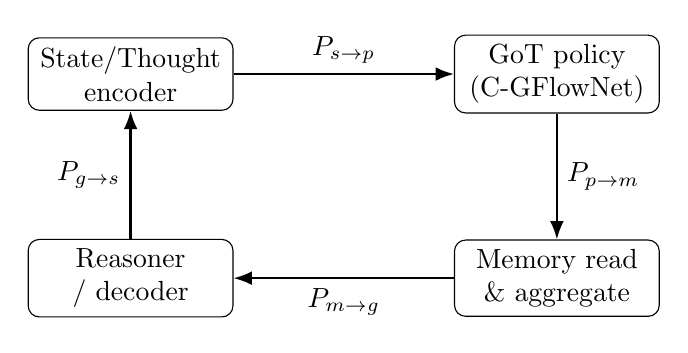
\begin{tikzpicture}[
  node/.style={draw, rounded corners, minimum width=2.6cm, minimum height=0.9cm, align=center},
  edge/.style={-Latex, thick}
]
\node[node] (q) {State/Thought\\encoder};
\node[node, right=2.8cm of q] (r) {GoT policy\\(C-GFlowNet)};
\node[node, below=1.6cm of r] (d) {Memory read\\\& aggregate};
\node[node, left=2.8cm of d] (g) {Reasoner\\ / decoder};

\draw[edge] (q) -- node[above] {$P_{s\to p}$} (r);
\draw[edge] (r) -- node[right] {$P_{p\to m}$} (d);
\draw[edge] (d) -- node[below] {$P_{m\to g}$} (g);
\draw[edge] (g) -- node[left] {$P_{g\to s}$} (q);
\end{tikzpicture}
\caption{Iterative GoT memory refinement as a cyclic decorated quiver.}
\end{figure}

\subsection{Tool-use agent loop}
A tool-use agent can be represented as a cycle between a controller, tool modules, and memory/state.
Stability diagnostics can be applied to learned state embeddings even when tools are non-differentiable.

\subsection{Protein design loop with multi-fidelity oracles}
A design loop cycles between proposal, prediction, and oracle evaluation:
GFlowNet proposal $\to$ predictors $\to$ acquisition policy $\to$ oracle $\to$ replay buffer $\to$ retrain predictors.
The key modeling advantage is that each predictor is a module with typed ports, enabling module swapping and interface diagnostics.

\section{Reference implementation outline}
\label{app:refimpl}

A minimal open-source implementation can be organized as:
\begin{itemize}[leftmargin=2em]
\item \texttt{quiver/graph.py}: data structures, SCC decomposition, execution backends,
\item \texttt{quiver/connectors.py}: connector templates and regularizers,
\item \texttt{quiver/solvers.py}: Anderson/Broyden fixed-point solvers and implicit gradients,
\item \texttt{quiver/diagnostics.py}: holonomy, norm, activation-fan, and tropical-cocycle tools,
\item \texttt{gflownet/}: graph-generation policies and trajectory balance losses,
\item \texttt{examples/}: case studies (GoT memory, MoE, world model, protein design).
\end{itemize}
Unit tests should cover: type checking, cycle basis extraction, holonomy computation, and solver convergence on toy graphs.



\section{Worked examples and experiment blueprints}
\label{app:worked}

This appendix provides concrete, end-to-end worked examples that can be implemented as sanity checks before scaling to large systems.
Each example includes: (i) a minimal quiver, (ii) recommended losses, (iii) diagnostics to log, and (iv) expected failure signatures.

\subsection{Example 1: Two-module alignment with a synthetic cycle}
\paragraph{Setup.}
Generate paired data $(x,y)$ from a ground-truth linear map $y=Tx+\epsilon$ with $x\in\R^{d_x}$, $y\in\R^{d_y}$.
Define two ``pretrained'' modules:
$N_a(x)=f(W_a x)$ and $N_b(y)=g(W_b y)$ with random frozen weights and nonlinearities.
We want to connect $N_a$ to $N_b$ via a connector $P_{a\to b}$ and create a synthetic cycle by adding a reconstruction connector $P_{b\to a}$.

\paragraph{Quiver.}
Vertices: $a$ and $b$.
Edges: $a\to b$ with $P_{a\to b}$, and $b\to a$ with $P_{b\to a}$.

\paragraph{Loss.}
Train connectors to minimize:
\[
L = \E\big[\norm{P_{a\to b}(N_a(x)) - N_b(y)}^2\big]
+ \lambda_{\mathrm{hol}} \Frob{P_{b\to a}P_{a\to b}-I}^2
+ \lambda_{\mathrm{iso}} L_{\mathrm{iso}}.
\]
Initialize $P_{a\to b}$ by ridge regression or CCA.

\paragraph{Diagnostics.}
Log $\opnorm{P_{a\to b}}$, $\opnorm{P_{b\to a}}$, holonomy defect $\Frob{P_{b\to a}P_{a\to b}-I}$, and training loss.
Expected behavior: holonomy decreases during training; norms remain bounded.
Failure signature: holonomy decreases but norms explode (ill-conditioned gauge drift), indicating need for orthogonality/partial-isometry constraints.

\subsection{Example 2: Cyclic SCC with fixed-point execution}
\paragraph{Setup.}
Define a three-node SCC:
\[
z_1 \xrightarrow{P_{1\to 2}} z_2 \xrightarrow{P_{2\to 3}} z_3 \xrightarrow{P_{3\to 1}} z_1,
\]
with each node applying a small MLP $N_i$.
Train the SCC to implement a known contraction mapping (e.g., solve $z=\tanh(Az+b)$ for random $A$ with $\rho(A)<1$).

\paragraph{Loss.}
Minimize the fixed-point residual:
\[
L_{\mathrm{fp}}=\E_{z_0}\norm{z^\star-\Phi(z^\star)}^2,
\]
plus connector norm penalties.

\paragraph{Diagnostics.}
Log solver residual vs iteration, estimated $\sigma_{\max}(D\Phi)$ (\cref{alg:power-jacobian}), and tropical growth from short trajectories.
Failure signature: residual stagnates and $\sigma_{\max}>1$, indicating the need for damping or stronger connector constraints.

\subsection{Example 3: Modular world-model + planner toy loop}
\paragraph{Setup.}
Construct a toy environment with latent state $s\in\R^d$ and dynamics $s_{t+1}=A s_t + B a_t$.
Implement:
encoder $N_e$, dynamics $N_f$, planner $N_p$, policy $N_\pi$ as modules.
Close the loop by feeding predicted future states back into the planner.

\paragraph{Goal.}
Recover a stable closed-loop system with desired spectral radius.

\paragraph{Loss and diagnostics.}
Use cellwise affine control fits on the closed-loop latent dynamics to estimate tropical growth and nearly absorbing subfans.
Penalize positive growth or excessive boundary congestion to stabilize planning.

\subsection{Example 4: Neural operator + corrector on a 1D PDE}
\paragraph{Setup.}
Use a simple PDE dataset (e.g., Burgers' equation).
Module $N_\mathrm{coarse}$ predicts a coarse solution; module $N_\mathrm{corr}$ predicts residual corrections; optionally, apply $N_\mathrm{corr}$ iteratively (cycle).
Connectors map between coarse and fine discretizations (linear interpolation matrices).

\paragraph{Diagnostics.}
Holonomy checks detect inconsistency between interpolation and restriction operators; tropical growth and activation occupancy quantify stability of iterative correction.

\subsection{Anderson acceleration (code)}
\begin{lstlisting}[language=Python,caption={Anderson acceleration for fixed-point solving in cyclic SCCs (minimal implementation).},label={lst:anderson}]
import torch

def anderson(phi, z0, m=5, max_iter=50, tol=1e-5, lam=1e-4):
    # z0: tensor or tuple of tensors; here assume a single tensor for brevity
    z = z0
    f = phi(z) - z
    X, F = [], []

    for k in range(max_iter):
        if torch.norm(f) < tol:
            break
        X.append(z); F.append(f)
        if len(X) > m:
            X.pop(0); F.pop(0)

        # Solve (F^T F + lam I) alpha = 1  (least squares on residuals)
        Fmat = torch.stack([fi.flatten() for fi in F], dim=1)  # (d, m)
        G = Fmat.T @ Fmat + lam * torch.eye(Fmat.shape[1], device=z.device)
        ones = torch.ones(Fmat.shape[1], device=z.device)
        alpha = torch.linalg.solve(G, ones)
        alpha = alpha / alpha.sum()

        z = sum(a * x for a, x in zip(alpha, X))
        z_next = phi(z)
        f = z_next - z
        z = z_next
    return z
\end{lstlisting}

\subsection{Recommended ablation protocol}
When evaluating the framework empirically, we recommend the following ablations:
\begin{enumerate}[leftmargin=2em]
\item \textbf{Connector-only vs. unfreeze modules:} quantify how much performance comes from interface learning alone.
\item \textbf{With vs. without holonomy penalty:} measure stability and performance for cyclic graphs.
\item \textbf{With vs. without tropical regularization:} measure cycle mixing/stability metrics and downstream quality.
\item \textbf{Connector template sweep:} dense vs low-rank vs partial-isometry constrained.
\item \textbf{Execution semantics:} unroll vs fixed-point, controlling compute.
\end{enumerate}

These ablations are implementable and directly test the paper's claims.



\section{Tropical stochastic and controlled modular cycles}
\label{app:tropical-estimation-controlled}

Many practical cyclic graphs are \emph{stochastic} (noise injection, dropout, diffusion) and/or \emph{controlled} (planning loops with actions).
This appendix extends the tropical discussion to these settings in a way that remains implementable.

\subsection{Stochastic dynamics and activation Markov chains}
Consider a stochastic update
\[
z_{t+1} \sim p(\cdot \mid z_t),
\]
induced by a cyclic subgraph that includes randomness (e.g., injected noise, sampling).
Logging activation labels produces a stochastic process on cells:
\[
C_t \in \Sigma_\Psi,\qquad
\mathbb{P}(C_{t+1}=D \mid C_t=C).
\]
The resulting transition kernel on occupied cells is the finite-state object that controls mixing, recurrence, and nearly absorbing subfans.
In addition, one can fit cellwise affine \emph{mean} dynamics
\[
\E[z_{t+1}\mid z_t\in C] \approx A_C z_t+b_C,
\]
by averaging within occupied cells.

\paragraph{Practical implication.}
For stochastic cycles, tropical growth rates reflect the \emph{mean dominant amplification} along random itineraries.
Mixing and contraction diagnostics remain useful, but should be interpreted as average-case indicators.
Large variance across rollouts indicates that additional stochastic diagnostics (e.g., conditional covariance propagation or boundary-hitting probabilities) may be needed.

\subsection{Controlled dynamics and control-dependent fans}
World models and planning loops induce controlled updates:
\[
z_{t+1} = \Psi(z_t, a_t),
\]
where $a_t$ is an action proposed by a planner/policy module.
A practical and widely used tropical approximation is a \emph{cellwise affine controlled model}:
\[
\ z_{t+1} \approx A_C z_t + B_C a_t + b_C,
\]
whenever $z_t$ lies in an activation cell $C$.
For richer control dependence one may refine the fan by splitting cells according to control regimes or by adding bilinear features $a_t\odot z_t$.
These are standard system-identification forms and are easy to fit by linear regression once the occupied cells are known.

\subsection{Cellwise control regression}
Given snapshots $(z_t,a_t,z_{t+1})$, define feature matrices
\[
X=[z_1,\dots,z_T],\quad
Y=[z_2,\dots,z_{T+1}],\quad
U=[a_1,\dots,a_T].
\]
Within each occupied cell $C$, fit $A_C,B_C,b_C$ by least squares:
\[
Y_C \approx A_C X_C + B_C U_C + b_C\mathbf{1}^\top.
\]
This can be solved by stacking:
\[
Y_C \approx [A_C\ B_C\ b_C]
\begin{bmatrix}
X_C\\ U_C\\ \mathbf{1}^\top
\end{bmatrix}.
\]
Regularization is recommended.

\begin{algorithm}[t]
\caption{Cellwise affine control fit for a controlled cyclic subgraph}
\label{alg:dmdc}
\begin{algorithmic}[1]
\Require snapshots $\{(z_t,a_t,z_{t+1},C_t)\}$, ridge $\lambda$, minimum cell count $m$
\For{each occupied cell $C$ with count at least $m$}
\State form $X_C,Y_C,U_C$ from snapshots with $C_t=C$
\State $W_C \gets \begin{bmatrix}X_C\\ U_C\\ \mathbf{1}^\top\end{bmatrix}$
\State solve $[A_C\ B_C\ b_C] \gets Y_C W_C^\top (W_C W_C^\top + \lambda I)^{-1}$
\EndFor
\State \Return $\{(A_C,B_C,b_C)\}_C$
\end{algorithmic}
\end{algorithm}

\begin{lstlisting}[language=Python,caption={Cellwise affine control fitting (ridge-regularized).},label={lst:dmdc}]
import torch

def fit_cellwise_control(Z, Z_next, U, cell_ids, lam=1e-4, min_count=8):
    models = {}
    cells = torch.as_tensor(cell_ids)
    ones = torch.ones(Z.shape[0], 1, device=Z.device, dtype=Z.dtype)
    for c in cells.unique():
        mask = cells == c
        if int(mask.sum()) < min_count:
            continue
        X = torch.cat([Z[mask], U[mask], ones[mask]], dim=1)  # (n, d+m+1)
        Y = Z_next[mask]                                      # (n, d)
        G = X.T @ X + lam * torch.eye(X.shape[1], device=Z.device)
        Theta = torch.linalg.solve(G, X.T @ Y)               # (d+m+1, d)
        models[int(c)] = Theta
    return models
\end{lstlisting}

\subsection{How this helps modular graph design}
Controlled tropical models provide:
\begin{itemize}[leftmargin=2em]
\item \textbf{Stability checks under control:} analyze cellwise contraction and control-dependent tropical growth for the occupied fan.
\item \textbf{Planning surrogates:} use cellwise affine models for fast rollouts during architecture search or for debugging.
\item \textbf{Interface debugging:} if $B_C$ is ill-conditioned or unstable on a subset of cells, the connector feeding actions into the dynamics module is likely misaligned in a geometrically localized way.
\end{itemize}

\subsection{Tropical view of diffusion-like stochastic cycles}
Diffusion samplers and Langevin dynamics are stochastic update rules of the form $z_{t+1}=z_t + \Delta(z_t,\xi_t)$.
Activation Markov chains and local tropical charts are a natural language for these dynamics.
In practice, we do not attempt to compute full transition tensors; instead we:
(i) track occupied subfans and boundary-hit rates,
(ii) estimate transition entropy and effective sample size, and
(iii) treat positive tropical growth or nearly absorbing cells as ``bottlenecks'' indicating poor mixing.
This perspective transfers directly to any iterative refinement cycle, diffusion or otherwise.



\section{Graph rewriting, connector fusion, and compilation}
\label{app:compilation}

Composable architectures invite \emph{graph rewriting}: once a modular graph works, we often want to simplify, compress, or specialize it for deployment.
Because connectors are linear/affine, many useful rewrites are implementable and verifiable with simple algebra.

\subsection{Fusing consecutive connectors}
If two connectors compose without an intervening nonlinear module, they can be fused.
For edges $e_1:u\to v$ and $e_2:v\to w$ where $v$ is a purely linear ``adapter'' node or an identity module,
\[
P_{e_2}\circ P_{e_1}(z) = A_2(A_1 z + b_1)+b_2 = (A_2A_1)z + (A_2 b_1+b_2).
\]
Thus, we can replace the two edges by a single connector with matrix $A_{12}=A_2A_1$ and bias $b_{12}=A_2b_1+b_2$.

\paragraph{Benefit.}
Connector fusion reduces latency and memory and improves numerical stability by eliminating redundant transformations.

\subsection{Pruning parallel edges and low-impact paths}
In mixture-of-paths graphs (\cref{sec:path-algebra}), many edges contribute negligibly.
A practical pruning criterion uses \emph{path contribution} metrics:
\begin{itemize}[leftmargin=2em]
\item average routing probability $\E[\pi_p(x)]$,
\item average message norm $\E[\norm{P_e(y_u)}]$,
\item gradient-based importance scores.
\end{itemize}
Edges below a threshold can be removed and the graph re-finetuned.

\subsection{Replacing a subgraph by a distilled module}
Given a subgraph $S$ with inputs $x$ and outputs $y_S(x)$, define a student module $\tilde N$ and train it by distillation:
\[
\min_{\tilde\theta}\ \E_x \norm{\tilde N_{\tilde\theta}(x)-y_S(x)}^2.
\]
This yields a new graph with fewer vertices and edges.
Because the quiver representation is explicit, identifying subgraphs and their interfaces is straightforward.

\subsection{Safety checks for rewrites}
We recommend verifying rewrites via:
\begin{itemize}[leftmargin=2em]
\item \textbf{interface checks:} port types and shapes match,
\item \textbf{functional tests:} compare outputs on a held-out validation set,
\item \textbf{invariant checks:} holonomy on remaining cycles does not increase, and connector norms remain bounded.
\end{itemize}

\subsection{Algorithm: linear connector fusion pass}
\begin{algorithm}[t]
\caption{Fuse consecutive linear connectors (local compilation pass)}
\label{alg:fuse}
\begin{algorithmic}[1]
\Require decorated quiver $g$
\For{each vertex $v$}
  \If{$v$ is linear/identity and has exactly one incoming edge $e_\mathrm{in}$ and one outgoing edge $e_\mathrm{out}$}
    \State compute fused connector parameters for $e_\mathrm{fuse}=e_\mathrm{out}\circ e_\mathrm{in}$
    \State remove $v,e_\mathrm{in},e_\mathrm{out}$ and insert $e_\mathrm{fuse}$
  \EndIf
\EndFor
\State \Return simplified graph
\end{algorithmic}
\end{algorithm}

This pass can be repeated until convergence.
More advanced compilation can fuse blocks of linear maps, push normalization into adjacent modules, or specialize tensor layouts for hardware kernels.

\section{References}
\label{sec:refs}

\begin{thebibliography}{99}

\bibitem{BaiDEQ}
S. Bai, J. Z. Kolter, and V. Koltun.
\newblock Deep equilibrium models.
\newblock \emph{NeurIPS}, 2019.

\bibitem{HuLoRA}
E. Hu, Y. Shen, P. Wallis, et al.
\newblock LoRA: Low-rank adaptation of large language models.
\newblock \emph{ICLR}, 2022.

\bibitem{HoulsbyAdapters}
N. Houlsby, A. Giurgiu, S. Jastrzebski, et al.
\newblock Parameter-efficient transfer learning for NLP.
\newblock \emph{ICML}, 2019.

\bibitem{YunBhojanapalliRawatKumarReddi2020}
C. Yun, S. Bhojanapalli, A. S. Rawat, S. Kumar, and S. J. Reddi.
\newblock Are transformers universal approximators of sequence-to-sequence functions?
\newblock \emph{ICLR}, 2020.

\bibitem{KimNguyenMinChoLeeLeeHong2022}
J. Kim, T. D. Nguyen, S. Min, S. Cho, M. Lee, H. Lee, and S. Hong.
\newblock Pure transformers are powerful graph learners.
\newblock \emph{NeurIPS}, 2022.

\bibitem{DauparasProteinMPNN2022}
J. Dauparas, I. Anishchenko, N. Bennett, H. Bai, R. J. Ragotte, et al.
\newblock Robust deep learning--based protein sequence design using {ProteinMPNN}.
\newblock \emph{Science}, 378(6615):49--56, 2022.

\bibitem{MarcolliChomskyBerwickMerge2023}
M. Marcolli, N. Chomsky, and R. C. Berwick.
\newblock Mathematical structure of syntactic merge.
\newblock \emph{arXiv:2305.18278}, 2023.

\bibitem{MarcolliBerwickChomskyMinimalism2023}
M. Marcolli, R. C. Berwick, and N. Chomsky.
\newblock Old and new minimalism: a {Hopf} algebra comparison.
\newblock \emph{arXiv:2306.10270}, 2023.

\bibitem{MarcolliBerwickChomskySyntaxSemantics2023}
M. Marcolli, R. C. Berwick, and N. Chomsky.
\newblock Syntax-semantics interface: an algebraic model.
\newblock \emph{arXiv:2311.06189}, 2023.

\bibitem{MarcolliPortGraphGrammars2015}
M. Marcolli and A. Port.
\newblock Graph grammars, insertion Lie algebras, and quantum field theory.
\newblock \emph{arXiv:1502.07796}, 2015.

\bibitem{AltabaaChenLaffertyYang2025}
A. Altabaa, S. Chen, J. Lafferty, and Z. Yang.
\newblock Unlocking out-of-distribution generalization in transformers via recursive latent space reasoning.
\newblock \emph{arXiv:2510.14095}, 2025.

\bibitem{AnthropicAssistantAxis2026}
Anthropic.
\newblock The assistant axis: Situating and stabilizing the character of large language models.
\newblock \url{https://www.anthropic.com/research/assistant-axis}, 2026.

\bibitem{LuGallagherMichalaFishLindsey2026}
C. Lu, J. Gallagher, J. Michala, K. Fish, and J. Lindsey.
\newblock The assistant axis: Situating and stabilizing the default persona of language models.
\newblock \emph{arXiv:2601.10387}, 2026.

\bibitem{HashemiPasqueTeskaYoshida2025}
B. Hashemi, K. Pasque, C. Teska, and R. Yoshida.
\newblock Tropical attention: Neural algorithmic reasoning for combinatorial algorithms.
\newblock \emph{arXiv:2505.17190}, 2025.

\bibitem{NatureLM2025}
NatureLM team.
\newblock Nature language model: Deciphering the language of nature for scientific discovery.
\newblock \emph{arXiv:2502.07527}, 2025.

\bibitem{MDGen2024}
\newblock Generative modeling of molecular dynamics trajectories.
\newblock \emph{arXiv:2409.17808}, 2024.

\bibitem{ZhangNaitzatLim2018}
L. Zhang, G. Naitzat, and L.-H. Lim.
\newblock Tropical geometry of deep neural networks.
\newblock \emph{ICML}, 2018.

\bibitem{BrandenburgLohoMontufar2024}
M.-C. Brandenburg, G. Loho, and G. Montufar.
\newblock The real tropical geometry of neural networks.
\newblock \emph{arXiv:2403.11871}, 2024.

\bibitem{MaclaganSturmfelsTropical}
D. Maclagan and B. Sturmfels.
\newblock \emph{Introduction to Tropical Geometry}.
\newblock American Mathematical Society, 2015.

\bibitem{FominWilliamsZelevinsky2016}
S. Fomin, L. Williams, and A. Zelevinsky.
\newblock Introduction to cluster algebras. Chapters 1--3.
\newblock \emph{arXiv:1608.05735}, 2016.

\bibitem{SchifflerClusterNotes}
R. Schiffler.
\newblock Cluster algebras and cluster categories.
\newblock Lecture notes for the Latin American Algebra Colloquium, 2009.

\bibitem{SchifflerQuiverReps}
R. Schiffler.
\newblock \emph{Quiver Representations}.
\newblock CMS Books in Mathematics, Springer, 2014.

\bibitem{KingmanSubadditive}
J. F. C. Kingman.
\newblock The ergodic theory of subadditive stochastic processes.
\newblock \emph{Journal of the Royal Statistical Society, Series B}, 30(3):499--510, 1968.

\bibitem{LiFNO}
Z. Li, N. Kovachki, K. Azizzadenesheli, et al.
\newblock Fourier neural operator for parametric PDEs.
\newblock \emph{ICLR}, 2021.

\bibitem{LuDeepONet}
L. Lu, P. Jin, and G. E. Karniadakis.
\newblock DeepONet: Learning nonlinear operators for PDEs.
\newblock \emph{arXiv}, 2019.

\bibitem{BengioGFlowNet}
Y. Bengio, T. Deleu, N. Malkin, et al.
\newblock Flow network based generative models for non-iterative diverse candidate generation.
\newblock \emph{NeurIPS Workshop}, 2021.

\bibitem{MalkinTB}
N. Malkin, M. B. Zhang, A. C. Le, et al.
\newblock Trajectory balance: Improved credit assignment in GFlowNets.
\newblock \emph{NeurIPS}, 2022.

\bibitem{BestaGoT}
M. Besta, N. Blach, A. Kubicek, et al.
\newblock Graph of thoughts: Solving elaborate problems with large language models.
\newblock \emph{AAAI}, 2024.

\bibitem{ShazeerMoE}
N. Shazeer, A. Mirhoseini, K. Maziarz, et al.
\newblock Outrageously large neural networks: The sparsely-gated mixture-of-experts layer.
\newblock \emph{ICLR}, 2017.

\bibitem{FedusSwitch}
W. Fedus, B. Zoph, and N. Shazeer.
\newblock Switch transformers: Scaling to trillion parameter models with simple and efficient sparsity.
\newblock \emph{JMLR}, 2022.

\bibitem{HoDDPM}
J. Ho, A. Jain, and P. Abbeel.
\newblock Denoising diffusion probabilistic models.
\newblock \emph{NeurIPS}, 2020.

\bibitem{SongScore}
Y. Song and S. Ermon.
\newblock Generative modeling by estimating gradients of the data distribution.
\newblock \emph{NeurIPS}, 2019.

\bibitem{AtiyahSingerIndex}
M.~F. Atiyah and I.~M. Singer.
\newblock The index of elliptic operators {I}.
\newblock {\em Annals of Mathematics}, 87(3):484--530, 1968.

\bibitem{ConnesNCG}
A.~Connes.
\newblock {\em Noncommutative Geometry}.
\newblock Academic Press, 1994.

\bibitem{WaltersErgodic}
P.~Walters.
\newblock {\em An Introduction to Ergodic Theory}.
\newblock Springer, 1982.

\bibitem{TemamNS}
R.~Temam.
\newblock {\em Navier--Stokes Equations: Theory and Numerical Analysis}.
\newblock North-Holland, 1977.

\bibitem{RaissiPINNs}
M.~Raissi, P.~Perdikaris, and G.~E. Karniadakis.
\newblock Physics-informed neural networks: a deep learning framework for solving forward and inverse problems involving nonlinear partial differential equations.
\newblock {\em Journal of Computational Physics}, 378:686--707, 2019.

\end{thebibliography}

\end{document}
